\documentclass[twoside]{book}

% Packages required by doxygen
\usepackage{fixltx2e}
\usepackage{calc}
\usepackage{doxygen}
\usepackage[export]{adjustbox} % also loads graphicx
\usepackage{graphicx}
\usepackage[utf8]{inputenc}
\usepackage{makeidx}
\usepackage{multicol}
\usepackage{multirow}
\PassOptionsToPackage{warn}{textcomp}
\usepackage{textcomp}
\usepackage[nointegrals]{wasysym}
\usepackage[table]{xcolor}

% Font selection
\usepackage[T1]{fontenc}
\usepackage[scaled=.90]{helvet}
\usepackage{courier}
\usepackage{amssymb}
\usepackage{sectsty}
\renewcommand{\familydefault}{\sfdefault}
\allsectionsfont{%
  \fontseries{bc}\selectfont%
  \color{darkgray}%
}
\renewcommand{\DoxyLabelFont}{%
  \fontseries{bc}\selectfont%
  \color{darkgray}%
}
\newcommand{\+}{\discretionary{\mbox{\scriptsize$\hookleftarrow$}}{}{}}

% Page & text layout
\usepackage{geometry}
\geometry{%
  a4paper,%
  top=2.5cm,%
  bottom=2.5cm,%
  left=2.5cm,%
  right=2.5cm%
}
\tolerance=750
\hfuzz=15pt
\hbadness=750
\setlength{\emergencystretch}{15pt}
\setlength{\parindent}{0cm}
\setlength{\parskip}{3ex plus 2ex minus 2ex}
\makeatletter
\renewcommand{\paragraph}{%
  \@startsection{paragraph}{4}{0ex}{-1.0ex}{1.0ex}{%
    \normalfont\normalsize\bfseries\SS@parafont%
  }%
}
\renewcommand{\subparagraph}{%
  \@startsection{subparagraph}{5}{0ex}{-1.0ex}{1.0ex}{%
    \normalfont\normalsize\bfseries\SS@subparafont%
  }%
}
\makeatother

% Headers & footers
\usepackage{fancyhdr}
\pagestyle{fancyplain}
\fancyhead[LE]{\fancyplain{}{\bfseries\thepage}}
\fancyhead[CE]{\fancyplain{}{}}
\fancyhead[RE]{\fancyplain{}{\bfseries\leftmark}}
\fancyhead[LO]{\fancyplain{}{\bfseries\rightmark}}
\fancyhead[CO]{\fancyplain{}{}}
\fancyhead[RO]{\fancyplain{}{\bfseries\thepage}}
\fancyfoot[LE]{\fancyplain{}{}}
\fancyfoot[CE]{\fancyplain{}{}}
\fancyfoot[RE]{\fancyplain{}{\bfseries\scriptsize Generated by Doxygen }}
\fancyfoot[LO]{\fancyplain{}{\bfseries\scriptsize Generated by Doxygen }}
\fancyfoot[CO]{\fancyplain{}{}}
\fancyfoot[RO]{\fancyplain{}{}}
\renewcommand{\footrulewidth}{0.4pt}
\renewcommand{\chaptermark}[1]{%
  \markboth{#1}{}%
}
\renewcommand{\sectionmark}[1]{%
  \markright{\thesection\ #1}%
}

% Indices & bibliography
\usepackage{natbib}
\usepackage[titles]{tocloft}
\setcounter{tocdepth}{3}
\setcounter{secnumdepth}{5}
\makeindex

% Hyperlinks (required, but should be loaded last)
\usepackage{ifpdf}
\ifpdf
  \usepackage[pdftex,pagebackref=true]{hyperref}
\else
  \usepackage[ps2pdf,pagebackref=true]{hyperref}
\fi
\hypersetup{%
  colorlinks=true,%
  linkcolor=blue,%
  citecolor=blue,%
  unicode%
}

% Custom commands
\newcommand{\clearemptydoublepage}{%
  \newpage{\pagestyle{empty}\cleardoublepage}%
}

\usepackage{caption}
\captionsetup{labelsep=space,justification=centering,font={bf},singlelinecheck=off,skip=4pt,position=top}

%===== C O N T E N T S =====

\begin{document}

% Titlepage & ToC
\hypersetup{pageanchor=false,
             bookmarksnumbered=true,
             pdfencoding=unicode
            }
\pagenumbering{roman}
\begin{titlepage}
\vspace*{7cm}
\begin{center}%
{\Large Gateware Libraries }\\
\vspace*{1cm}
{\large Generated by Doxygen 1.8.11}\\
\end{center}
\end{titlepage}
\clearemptydoublepage
\tableofcontents
\clearemptydoublepage
\pagenumbering{arabic}
\hypersetup{pageanchor=true}

%--- Begin generated contents ---
\chapter{Gateware Libraries}
\label{index}\hypertarget{index}{}\begin{DoxyCopyright}{Copyright}
Copyright (c) 2016 7th\+Gate Software .L\+LC 
\end{DoxyCopyright}
\begin{DoxyParagraph}{License\+:}
Gateware libraries are released under Creative Commons M\+IT lincense unless noted differently by the library. 
\end{DoxyParagraph}
\begin{DoxyVersion}{Version}
Beta Release
\end{DoxyVersion}
\hypertarget{index_API}{}\section{A\+P\+I\+Overview}\label{index_API}
Coming Soon\hypertarget{index_APIOverview}{}\subsection{G\+Log}\label{index_APIOverview}
Coming Soon\hypertarget{index_GLog}{}\subsection{G\+File}\label{index_GLog}
Coming Soon\hypertarget{index_GFile}{}\subsection{G\+Input}\label{index_GFile}
Coming Soon\hypertarget{index_GInput}{}\subsection{G\+Buffered\+Input}\label{index_GInput}
Coming Soon\hypertarget{index_Installation}{}\section{Installation}\label{index_Installation}
Coming Soon\hypertarget{index_Bug}{}\section{Reporting}\label{index_Bug}
Coming Soon 
\chapter{L\+I\+C\+E\+N\+SE}
\label{md_LICENSE}
\hypertarget{md_LICENSE}{}
The M\+IT License (M\+IT)

Copyright (c) 2016 7th\+Gate Software .L\+LC

Permission is hereby granted, free of charge, to any person obtaining a copy of this software and associated documentation files (the \char`\"{}\+Software\char`\"{}), to deal in the Software without restriction, including without limitation the rights to use, copy, modify, merge, publish, distribute, sublicense, and/or sell copies of the Software, and to permit persons to whom the Software is furnished to do so, subject to the following conditions\+:

The above copyright notice and this permission notice shall be included in all copies or substantial portions of the Software.

T\+HE S\+O\+F\+T\+W\+A\+RE IS P\+R\+O\+V\+I\+D\+ED \char`\"{}\+A\+S I\+S\char`\"{}, W\+I\+T\+H\+O\+UT W\+A\+R\+R\+A\+N\+TY OF A\+NY K\+I\+ND, E\+X\+P\+R\+E\+SS OR I\+M\+P\+L\+I\+ED, I\+N\+C\+L\+U\+D\+I\+NG B\+UT N\+OT L\+I\+M\+I\+T\+ED TO T\+HE W\+A\+R\+R\+A\+N\+T\+I\+ES OF M\+E\+R\+C\+H\+A\+N\+T\+A\+B\+I\+L\+I\+TY, F\+I\+T\+N\+E\+SS F\+OR A P\+A\+R\+T\+I\+C\+U\+L\+AR P\+U\+R\+P\+O\+SE A\+ND N\+O\+N\+I\+N\+F\+R\+I\+N\+G\+E\+M\+E\+NT. IN NO E\+V\+E\+NT S\+H\+A\+LL T\+HE A\+U\+T\+H\+O\+RS OR C\+O\+P\+Y\+R\+I\+G\+HT H\+O\+L\+D\+E\+RS BE L\+I\+A\+B\+LE F\+OR A\+NY C\+L\+A\+IM, D\+A\+M\+A\+G\+ES OR O\+T\+H\+ER L\+I\+A\+B\+I\+L\+I\+TY, W\+H\+E\+T\+H\+ER IN AN A\+C\+T\+I\+ON OF C\+O\+N\+T\+R\+A\+CT, T\+O\+RT OR O\+T\+H\+E\+R\+W\+I\+SE, A\+R\+I\+S\+I\+NG F\+R\+OM, O\+UT OF OR IN C\+O\+N\+N\+E\+C\+T\+I\+ON W\+I\+TH T\+HE S\+O\+F\+T\+W\+A\+RE OR T\+HE U\+SE OR O\+T\+H\+ER D\+E\+A\+L\+I\+N\+GS IN T\+HE S\+O\+F\+T\+W\+A\+RE. 
\chapter{R\+E\+A\+D\+ME}
\label{md_README}
\hypertarget{md_README}{}
Gateware Libraries

This is currently Beta released code. This code is subject to Interface Changes and bugs.

Please report any bugs with this build to underdog specifing the revision number. Revision number\# 78f9e2 
\chapter{Namespace Index}
\section{Namespace List}
Here is a list of all documented namespaces with brief descriptions\+:\begin{DoxyCompactList}
\item\contentsline{section}{\mbox{\hyperlink{namespace_g_w}{GW}} \\*The core namespace to which all Gateware interfaces/structures/defines must belong }{\pageref{namespace_g_w}}{}
\item\contentsline{section}{\mbox{\hyperlink{namespace_g_w_1_1_a_u_d_i_o}{G\+W\+::\+A\+U\+D\+IO}} \\*The namespace to which all Gateware library interfaces must belong }{\pageref{namespace_g_w_1_1_a_u_d_i_o}}{}
\item\contentsline{section}{\mbox{\hyperlink{namespace_g_w_1_1_c_o_r_e}{G\+W\+::\+C\+O\+RE}} \\*The core namespace to which all Gateware fundamental interfaces must belong }{\pageref{namespace_g_w_1_1_c_o_r_e}}{}
\item\contentsline{section}{\mbox{\hyperlink{namespace_g_w_1_1_g_r_a_p_h_i_c_s}{G\+W\+::\+G\+R\+A\+P\+H\+I\+CS}} \\*The namespace to which all Gateware Graphics library interfaces must belong }{\pageref{namespace_g_w_1_1_g_r_a_p_h_i_c_s}}{}
\item\contentsline{section}{\mbox{\hyperlink{namespace_g_w_1_1_m_a_t_h}{G\+W\+::\+M\+A\+TH}} \\*The namespace to which all math library interface must belong }{\pageref{namespace_g_w_1_1_m_a_t_h}}{}
\item\contentsline{section}{\mbox{\hyperlink{namespace_g_w_1_1_s_y_s_t_e_m}{G\+W\+::\+S\+Y\+S\+T\+EM}} \\*The namespace to which all Gateware library interfaces must belong }{\pageref{namespace_g_w_1_1_s_y_s_t_e_m}}{}
\end{DoxyCompactList}

\chapter{Hierarchical Index}
\section{Class Hierarchy}
This inheritance list is sorted roughly, but not completely, alphabetically\+:\begin{DoxyCompactList}
\item \contentsline{section}{GW\+:\+:S\+Y\+S\+T\+EM\+:\+:G\+B\+U\+F\+F\+E\+R\+E\+D\+I\+N\+P\+U\+T\+\_\+\+E\+V\+E\+N\+T\+\_\+\+D\+A\+TA}{\pageref{struct_g_w_1_1_s_y_s_t_e_m_1_1_g_b_u_f_f_e_r_e_d_i_n_p_u_t___e_v_e_n_t___d_a_t_a}}{}
\item \contentsline{section}{GW\+:\+:S\+Y\+S\+T\+EM\+:\+:G\+C\+O\+N\+T\+R\+O\+L\+L\+E\+R\+\_\+\+E\+V\+E\+N\+T\+\_\+\+D\+A\+TA}{\pageref{struct_g_w_1_1_s_y_s_t_e_m_1_1_g_c_o_n_t_r_o_l_l_e_r___e_v_e_n_t___d_a_t_a}}{}
\item \contentsline{section}{GW\+:\+:C\+O\+RE\+:\+:G\+Interface}{\pageref{class_g_w_1_1_c_o_r_e_1_1_g_interface}}{}
\begin{DoxyCompactList}
\item \contentsline{section}{GW\+:\+:C\+O\+RE\+:\+:G\+Multi\+Threaded}{\pageref{class_g_w_1_1_c_o_r_e_1_1_g_multi_threaded}}{}
\begin{DoxyCompactList}
\item \contentsline{section}{GW\+:\+:A\+U\+D\+IO\+:\+:G\+Audio}{\pageref{class_g_w_1_1_a_u_d_i_o_1_1_g_audio}}{}
\item \contentsline{section}{GW\+:\+:A\+U\+D\+IO\+:\+:G\+Music}{\pageref{class_g_w_1_1_a_u_d_i_o_1_1_g_music}}{}
\item \contentsline{section}{GW\+:\+:A\+U\+D\+IO\+:\+:G\+Sound}{\pageref{class_g_w_1_1_a_u_d_i_o_1_1_g_sound}}{}
\item \contentsline{section}{GW\+:\+:C\+O\+RE\+:\+:G\+Broadcasting}{\pageref{class_g_w_1_1_c_o_r_e_1_1_g_broadcasting}}{}
\begin{DoxyCompactList}
\item \contentsline{section}{GW\+:\+:S\+Y\+S\+T\+EM\+:\+:G\+Buffered\+Input}{\pageref{class_g_w_1_1_s_y_s_t_e_m_1_1_g_buffered_input}}{}
\item \contentsline{section}{GW\+:\+:S\+Y\+S\+T\+EM\+:\+:G\+Controller}{\pageref{class_g_w_1_1_s_y_s_t_e_m_1_1_g_controller}}{}
\item \contentsline{section}{GW\+:\+:S\+Y\+S\+T\+EM\+:\+:G\+Window}{\pageref{class_g_w_1_1_s_y_s_t_e_m_1_1_g_window}}{}
\end{DoxyCompactList}
\item \contentsline{section}{GW\+:\+:C\+O\+RE\+:\+:G\+Listener}{\pageref{class_g_w_1_1_c_o_r_e_1_1_g_listener}}{}
\begin{DoxyCompactList}
\item \contentsline{section}{GW\+:\+:G\+R\+A\+P\+H\+I\+CS\+:\+:G\+Direct\+X11\+Surface}{\pageref{class_g_w_1_1_g_r_a_p_h_i_c_s_1_1_g_direct_x11_surface}}{}
\item \contentsline{section}{GW\+:\+:G\+R\+A\+P\+H\+I\+CS\+:\+:G\+Open\+G\+L\+Surface}{\pageref{class_g_w_1_1_g_r_a_p_h_i_c_s_1_1_g_open_g_l_surface}}{}
\end{DoxyCompactList}
\item \contentsline{section}{GW\+:\+:S\+Y\+S\+T\+EM\+:\+:G\+File}{\pageref{class_g_w_1_1_s_y_s_t_e_m_1_1_g_file}}{}
\item \contentsline{section}{GW\+:\+:S\+Y\+S\+T\+EM\+:\+:G\+Log}{\pageref{class_g_w_1_1_s_y_s_t_e_m_1_1_g_log}}{}
\end{DoxyCompactList}
\item \contentsline{section}{GW\+:\+:C\+O\+RE\+:\+:G\+Single\+Threaded}{\pageref{class_g_w_1_1_c_o_r_e_1_1_g_single_threaded}}{}
\begin{DoxyCompactList}
\item \contentsline{section}{GW\+:\+:M\+A\+TH\+:\+:G\+Matrix}{\pageref{class_g_w_1_1_m_a_t_h_1_1_g_matrix}}{}
\item \contentsline{section}{GW\+:\+:M\+A\+TH\+:\+:G\+Quaternion}{\pageref{class_g_w_1_1_m_a_t_h_1_1_g_quaternion}}{}
\item \contentsline{section}{GW\+:\+:M\+A\+TH\+:\+:G\+Vector}{\pageref{class_g_w_1_1_m_a_t_h_1_1_g_vector}}{}
\item \contentsline{section}{GW\+:\+:S\+Y\+S\+T\+EM\+:\+:G\+Input}{\pageref{class_g_w_1_1_s_y_s_t_e_m_1_1_g_input}}{}
\end{DoxyCompactList}
\end{DoxyCompactList}
\item \contentsline{section}{GW\+:\+:M\+A\+TH\+:\+:G\+M\+A\+T\+R\+I\+XD}{\pageref{struct_g_w_1_1_m_a_t_h_1_1_g_m_a_t_r_i_x_d}}{}
\item \contentsline{section}{GW\+:\+:M\+A\+TH\+:\+:G\+M\+A\+T\+R\+I\+XF}{\pageref{struct_g_w_1_1_m_a_t_h_1_1_g_m_a_t_r_i_x_f}}{}
\item \contentsline{section}{GW\+:\+:M\+A\+TH\+:\+:G\+Q\+U\+A\+T\+E\+R\+N\+I\+O\+ND}{\pageref{struct_g_w_1_1_m_a_t_h_1_1_g_q_u_a_t_e_r_n_i_o_n_d}}{}
\item \contentsline{section}{GW\+:\+:M\+A\+TH\+:\+:G\+Q\+U\+A\+T\+E\+R\+N\+I\+O\+NF}{\pageref{struct_g_w_1_1_m_a_t_h_1_1_g_q_u_a_t_e_r_n_i_o_n_f}}{}
\item \contentsline{section}{GW\+:\+:G\+U\+U\+I\+ID}{\pageref{struct_g_w_1_1_g_u_u_i_i_d}}{}
\item \contentsline{section}{GW\+:\+:M\+A\+TH\+:\+:G\+V\+E\+C\+T\+O\+RD}{\pageref{struct_g_w_1_1_m_a_t_h_1_1_g_v_e_c_t_o_r_d}}{}
\item \contentsline{section}{GW\+:\+:M\+A\+TH\+:\+:G\+V\+E\+C\+T\+O\+RF}{\pageref{struct_g_w_1_1_m_a_t_h_1_1_g_v_e_c_t_o_r_f}}{}
\item \contentsline{section}{GW\+:\+:S\+Y\+S\+T\+EM\+:\+:G\+W\+I\+N\+D\+O\+W\+\_\+\+E\+V\+E\+N\+T\+\_\+\+D\+A\+TA}{\pageref{struct_g_w_1_1_s_y_s_t_e_m_1_1_g_w_i_n_d_o_w___e_v_e_n_t___d_a_t_a}}{}
\item \contentsline{section}{GW\+:\+:S\+Y\+S\+T\+EM\+:\+:L\+I\+N\+U\+X\+\_\+\+W\+I\+N\+D\+OW}{\pageref{struct_g_w_1_1_s_y_s_t_e_m_1_1_l_i_n_u_x___w_i_n_d_o_w}}{}
\end{DoxyCompactList}

\chapter{Class Index}
\section{Class List}
Here are the classes, structs, unions and interfaces with brief descriptions\+:\begin{DoxyCompactList}
\item\contentsline{section}{\mbox{\hyperlink{classGW_1_1AUDIO_1_1GAudio}{G\+W\+::\+A\+U\+D\+I\+O\+::\+G\+Audio}} }{\pageref{classGW_1_1AUDIO_1_1GAudio}}{}
\item\contentsline{section}{\mbox{\hyperlink{classGW_1_1CORE_1_1GBroadcasting}{G\+W\+::\+C\+O\+R\+E\+::\+G\+Broadcasting}} \\*The \mbox{\hyperlink{classGW_1_1CORE_1_1GBroadcasting}{G\+Broadcasting}} Interface is capable of registering \& deregistering \mbox{\hyperlink{classGW_1_1CORE_1_1GListener}{G\+Listener}} interfaces }{\pageref{classGW_1_1CORE_1_1GBroadcasting}}{}
\item\contentsline{section}{\mbox{\hyperlink{classGW_1_1SYSTEM_1_1GBufferedInput}{G\+W\+::\+S\+Y\+S\+T\+E\+M\+::\+G\+Buffered\+Input}} \\*A Multi-\/threaded buffered input library }{\pageref{classGW_1_1SYSTEM_1_1GBufferedInput}}{}
\item\contentsline{section}{\mbox{\hyperlink{structGW_1_1SYSTEM_1_1GBUFFEREDINPUT__EVENT__DATA}{G\+W\+::\+S\+Y\+S\+T\+E\+M\+::\+G\+B\+U\+F\+F\+E\+R\+E\+D\+I\+N\+P\+U\+T\+\_\+\+E\+V\+E\+N\+T\+\_\+\+D\+A\+TA}} \\*Ensure identical binary padding for structures on all platforms }{\pageref{structGW_1_1SYSTEM_1_1GBUFFEREDINPUT__EVENT__DATA}}{}
\item\contentsline{section}{\mbox{\hyperlink{classGW_1_1GRAPHICS_1_1GDirectX11Surface}{G\+W\+::\+G\+R\+A\+P\+H\+I\+C\+S\+::\+G\+Direct\+X11\+Surface}} \\*A library used to initialize, create, and manage a Direct\+X11 rendering context }{\pageref{classGW_1_1GRAPHICS_1_1GDirectX11Surface}}{}
\item\contentsline{section}{\mbox{\hyperlink{classGW_1_1SYSTEM_1_1GFile}{G\+W\+::\+S\+Y\+S\+T\+E\+M\+::\+G\+File}} \\*Cross platform File\+I\+O/\+Directory handling }{\pageref{classGW_1_1SYSTEM_1_1GFile}}{}
\item\contentsline{section}{\mbox{\hyperlink{classGW_1_1SYSTEM_1_1GInput}{G\+W\+::\+S\+Y\+S\+T\+E\+M\+::\+G\+Input}} \\*A single threaded input library }{\pageref{classGW_1_1SYSTEM_1_1GInput}}{}
\item\contentsline{section}{\mbox{\hyperlink{classGW_1_1CORE_1_1GInterface}{G\+W\+::\+C\+O\+R\+E\+::\+G\+Interface}} \\*Base interface all Gateware interfaces must support at a minimum }{\pageref{classGW_1_1CORE_1_1GInterface}}{}
\item\contentsline{section}{\mbox{\hyperlink{classGW_1_1CORE_1_1GListener}{G\+W\+::\+C\+O\+R\+E\+::\+G\+Listener}} \\*A \mbox{\hyperlink{classGW_1_1CORE_1_1GListener}{G\+Listener}} Interface may be registered with a G\+Broadcaster interface to receive event notifications }{\pageref{classGW_1_1CORE_1_1GListener}}{}
\item\contentsline{section}{\mbox{\hyperlink{classGW_1_1SYSTEM_1_1GLog}{G\+W\+::\+S\+Y\+S\+T\+E\+M\+::\+G\+Log}} \\*Cross platform threadsafe logger }{\pageref{classGW_1_1SYSTEM_1_1GLog}}{}
\item\contentsline{section}{\mbox{\hyperlink{classGW_1_1MATH_1_1GMatrix}{G\+W\+::\+M\+A\+T\+H\+::\+G\+Matrix}} \\*Matrix functions }{\pageref{classGW_1_1MATH_1_1GMatrix}}{}
\item\contentsline{section}{\mbox{\hyperlink{structGW_1_1MATH_1_1GMATRIXD}{G\+W\+::\+M\+A\+T\+H\+::\+G\+M\+A\+T\+R\+I\+XD}} \\*Matrix with 4 double vectors which represent for each row }{\pageref{structGW_1_1MATH_1_1GMATRIXD}}{}
\item\contentsline{section}{\mbox{\hyperlink{structGW_1_1MATH_1_1GMATRIXF}{G\+W\+::\+M\+A\+T\+H\+::\+G\+M\+A\+T\+R\+I\+XF}} \\*Matrix with 4 float vectors which represent for each row }{\pageref{structGW_1_1MATH_1_1GMATRIXF}}{}
\item\contentsline{section}{\mbox{\hyperlink{classGW_1_1CORE_1_1GMultiThreaded}{G\+W\+::\+C\+O\+R\+E\+::\+G\+Multi\+Threaded}} \\*This interface is only used to label and query interfaces which promise to 100\% internally support thread safety }{\pageref{classGW_1_1CORE_1_1GMultiThreaded}}{}
\item\contentsline{section}{\mbox{\hyperlink{classGW_1_1AUDIO_1_1GMusic}{G\+W\+::\+A\+U\+D\+I\+O\+::\+G\+Music}} }{\pageref{classGW_1_1AUDIO_1_1GMusic}}{}
\item\contentsline{section}{\mbox{\hyperlink{classGW_1_1GRAPHICS_1_1GOpenGLSurface}{G\+W\+::\+G\+R\+A\+P\+H\+I\+C\+S\+::\+G\+Open\+G\+L\+Surface}} \\*A library used to initialize, create, and manage an Open\+GL rendering context }{\pageref{classGW_1_1GRAPHICS_1_1GOpenGLSurface}}{}
\item\contentsline{section}{\mbox{\hyperlink{classGW_1_1MATH_1_1GQuaternion}{G\+W\+::\+M\+A\+T\+H\+::\+G\+Quaternion}} \\*Quaternion functions }{\pageref{classGW_1_1MATH_1_1GQuaternion}}{}
\item\contentsline{section}{\mbox{\hyperlink{structGW_1_1MATH_1_1GQUATERNIOND}{G\+W\+::\+M\+A\+T\+H\+::\+G\+Q\+U\+A\+T\+E\+R\+N\+I\+O\+ND}} \\*Quaternion with 4 double elements }{\pageref{structGW_1_1MATH_1_1GQUATERNIOND}}{}
\item\contentsline{section}{\mbox{\hyperlink{structGW_1_1MATH_1_1GQUATERNIONF}{G\+W\+::\+M\+A\+T\+H\+::\+G\+Q\+U\+A\+T\+E\+R\+N\+I\+O\+NF}} \\*Quaternion with 4 float elements }{\pageref{structGW_1_1MATH_1_1GQUATERNIONF}}{}
\item\contentsline{section}{\mbox{\hyperlink{classGW_1_1CORE_1_1GSingleThreaded}{G\+W\+::\+C\+O\+R\+E\+::\+G\+Single\+Threaded}} \\*This interface is only used to label and query interfaces which are not designed internally to support thread safety }{\pageref{classGW_1_1CORE_1_1GSingleThreaded}}{}
\item\contentsline{section}{\mbox{\hyperlink{classGW_1_1AUDIO_1_1GSound}{G\+W\+::\+A\+U\+D\+I\+O\+::\+G\+Sound}} }{\pageref{classGW_1_1AUDIO_1_1GSound}}{}
\item\contentsline{section}{\mbox{\hyperlink{structGW_1_1GUUIID}{G\+W\+::\+G\+U\+U\+I\+ID}} \\*Gateware Universally Unique Interface I\+Dentifier }{\pageref{structGW_1_1GUUIID}}{}
\item\contentsline{section}{\mbox{\hyperlink{classGW_1_1MATH_1_1GVector}{G\+W\+::\+M\+A\+T\+H\+::\+G\+Vector}} \\*Vector functions }{\pageref{classGW_1_1MATH_1_1GVector}}{}
\item\contentsline{section}{\mbox{\hyperlink{structGW_1_1MATH_1_1GVECTORD}{G\+W\+::\+M\+A\+T\+H\+::\+G\+V\+E\+C\+T\+O\+RD}} \\*Vector with 4 double elements }{\pageref{structGW_1_1MATH_1_1GVECTORD}}{}
\item\contentsline{section}{\mbox{\hyperlink{structGW_1_1MATH_1_1GVECTORF}{G\+W\+::\+M\+A\+T\+H\+::\+G\+V\+E\+C\+T\+O\+RF}} \\*To hold all math structs and variables }{\pageref{structGW_1_1MATH_1_1GVECTORF}}{}
\item\contentsline{section}{\mbox{\hyperlink{classGW_1_1SYSTEM_1_1GWindow}{G\+W\+::\+S\+Y\+S\+T\+E\+M\+::\+G\+Window}} \\*A thread-\/safe window creation and management library }{\pageref{classGW_1_1SYSTEM_1_1GWindow}}{}
\item\contentsline{section}{\mbox{\hyperlink{structGW_1_1SYSTEM_1_1GWINDOW__EVENT__DATA}{G\+W\+::\+S\+Y\+S\+T\+E\+M\+::\+G\+W\+I\+N\+D\+O\+W\+\_\+\+E\+V\+E\+N\+T\+\_\+\+D\+A\+TA}} \\*Ensure identical binary padding for structures on all platforms }{\pageref{structGW_1_1SYSTEM_1_1GWINDOW__EVENT__DATA}}{}
\item\contentsline{section}{\mbox{\hyperlink{structGW_1_1SYSTEM_1_1LINUX__WINDOW}{G\+W\+::\+S\+Y\+S\+T\+E\+M\+::\+L\+I\+N\+U\+X\+\_\+\+W\+I\+N\+D\+OW}} \\*The structure used to pass into Input libraries on Linux }{\pageref{structGW_1_1SYSTEM_1_1LINUX__WINDOW}}{}
\end{DoxyCompactList}

\chapter{Namespace Documentation}
\hypertarget{namespaceGW}{}\section{GW Namespace Reference}
\label{namespaceGW}\index{GW@{GW}}


The core namespace to which all Gateware interfaces/structures/defines must belong.  


\subsection*{Namespaces}
\begin{DoxyCompactItemize}
\item 
 \hyperlink{namespaceGW_1_1CORE}{C\+O\+RE}
\begin{DoxyCompactList}\small\item\em The core namespace to which all Gateware fundamental interfaces must belong. \end{DoxyCompactList}\item 
 \hyperlink{namespaceGW_1_1SYSTEM}{S\+Y\+S\+T\+EM}
\begin{DoxyCompactList}\small\item\em The namespace to which all Gateware library interfaces must belong. \end{DoxyCompactList}\end{DoxyCompactItemize}
\subsection*{Classes}
\begin{DoxyCompactItemize}
\item 
struct \hyperlink{structGW_1_1GUUIID}{G\+U\+U\+I\+ID}
\begin{DoxyCompactList}\small\item\em Gateware Universally Unique Interface I\+Dentifier. \end{DoxyCompactList}\end{DoxyCompactItemize}
\subsection*{Enumerations}
\begin{DoxyCompactItemize}
\item 
enum \hyperlink{namespaceGW_a67a839e3df7ea8a5c5686613a7a3de21}{G\+Return} \{ \\*
{\bfseries S\+U\+C\+C\+E\+SS} = 0x\+F\+F\+F\+F\+F\+F\+FF, 
{\bfseries F\+A\+I\+L\+U\+RE} = 0, 
{\bfseries I\+N\+V\+A\+L\+I\+D\+\_\+\+A\+R\+G\+U\+M\+E\+NT} = 1, 
{\bfseries M\+E\+M\+O\+R\+Y\+\_\+\+C\+O\+R\+R\+U\+P\+T\+I\+ON} = 2, 
\\*
{\bfseries I\+N\+T\+E\+R\+F\+A\+C\+E\+\_\+\+U\+N\+S\+U\+P\+P\+O\+R\+T\+ED} = 3, 
{\bfseries F\+I\+L\+E\+\_\+\+N\+O\+T\+\_\+\+F\+O\+U\+ND} = 4, 
{\bfseries R\+E\+D\+U\+N\+D\+A\+N\+T\+\_\+\+O\+P\+E\+R\+A\+T\+I\+ON} = 5, 
{\bfseries F\+E\+A\+T\+U\+R\+E\+\_\+\+U\+N\+S\+U\+P\+P\+O\+R\+T\+ED} = 6
 \}\hypertarget{namespaceGW_a67a839e3df7ea8a5c5686613a7a3de21}{}\label{namespaceGW_a67a839e3df7ea8a5c5686613a7a3de21}
\begin{DoxyCompactList}\small\item\em Listing of common error codes returned by Gateware functions. \end{DoxyCompactList}
\end{DoxyCompactItemize}


\subsection{Detailed Description}
The core namespace to which all Gateware interfaces/structures/defines must belong. 

G\+Input inherits directly from G\+Single\+Threaded.

G\+File inherits directly from G\+Multi\+Threaded.

G\+Buffered\+Input inherits directly from G\+Broadcasting.

G\+Single\+Threaded inherits directly from G\+Interface.

G\+Multi\+Threaded inherits directly from G\+Interface.

G\+Listener inherits directly from G\+Multi\+Threaded.

Contains all defined elements shared among base interfaces.

The core namespace to which all Gateware interfaces must belong.

File\+: \hyperlink{GBroadcasting_8h_source}{G\+Broadcasting.\+h} Purpose\+: A Gateware interface that allows an object derived from G\+Listener to receive select events from a G\+Broadcaster. Author\+: Lari H. Norri Contributors\+: N/A Last Modified\+: 10/13/2016 Interface Status\+: Final Copyright\+: 7th\+Gate Software L\+LC. License\+: M\+IT

File\+: \hyperlink{GDefines_8h_source}{G\+Defines.\+h} Purpose\+: Lists the core \#defines and M\+A\+C\+R\+OS used by the Gateware interfaces. Author\+: Lari H. Norri Contributors\+: N/A Last Modified\+: 12/12/2016 Copyright\+: 7th\+Gate Software L\+LC. License\+: M\+IT

File\+: \hyperlink{GInterface_8h_source}{G\+Interface.\+h} Purpose\+: The fundamental interface which all Gateware interfaces must adhere to at a minimum. Author\+: Lari H. Norri Contributors\+: N/A Last Modified\+: 9/29/2016 Interface Status\+: Final Copyright\+: 7th\+Gate Software L\+LC. License\+: M\+I\+T\+The core namespace to which all Gateware interfaces/structures/defines must belong.

File\+: \hyperlink{GListener_8h_source}{G\+Listener.\+h} Purpose\+: A Gateware interface that can safely listen \& respond to events sent from a G\+Broadcating interface. Author\+: Lari H. Norri Contributors\+: N/A Last Modified\+: 10/13/2016 Interface Status\+: Final Copyright\+: 7th\+Gate Software L\+LC. License\+: M\+I\+T\+The core namespace to which all Gateware interfaces/structures/defines must belong.

File\+: \hyperlink{GMultiThreaded_8h_source}{G\+Multi\+Threaded.\+h} Purpose\+: Indentifies any Gateware interface which is guaranteed to be safely accessed across multiple threads. Author\+: Lari H. Norri Contributors\+: N/A Last Modified\+: 10/13/2016 Interface Status\+: Final Copyright\+: 7th\+Gate Software L\+LC. License\+: M\+I\+T\+The core namespace to which all Gateware interfaces/structures/defines must belong.

File\+: \hyperlink{GSingleThreaded_8h_source}{G\+Single\+Threaded.\+h} Purpose\+: Indentifies any Gateware interface which may N\+OT be safely accessed across multiple threads. Author\+: Lari H. Norri Contributors\+: N/A Last Modified\+: 10/13/2016 Interface Status\+: Final Copyright\+: 7th\+Gate Software L\+LC. License\+: M\+I\+T\+The core namespace to which all Gateware interfaces/structures/defines must belong.

File\+: \hyperlink{GBufferedInput_8h_source}{G\+Buffered\+Input.\+h} Purpose\+: This Interface offers event based thread safe raw buffered input. Author\+: Peter Farber Contributors\+: N/A Last Modified\+: 11/16/2016 Interface Status\+: Beta Copyright\+: 7th\+Gate Software L\+LC. License\+: M\+I\+T\+The core namespace to which all Gateware interfaces/structures/defines must belong.

File\+: \hyperlink{GFile_8h_source}{G\+File.\+h} Purpose\+: A Gateware interface that handles both binary and textual file io and directory. Author\+: Justin W. Parks Contributors\+: N/A Last Modified\+: 11/16/2016 Interface Status\+: Beta Copyright\+: 7th\+Gate Software L\+LC. License\+: M\+I\+T\+The core namespace to which all Gateware interfaces/structures/defines must belong.

File\+: \hyperlink{GInput_8h_source}{G\+Input.\+h} Purpose\+: A Gateware interface that handles high-\/speed keyboard and mouse input. Author\+: Peter Farber Contributors\+: N/A Last Modified\+: 2/1/2017 Interface Status\+: Beta Copyright\+: 7th\+Gate Software L\+LC. License\+: M\+I\+T\+The core namespace to which all Gateware interfaces/structures/defines must belong.

File\+: \hyperlink{GLog_8h_source}{G\+Log.\+h} Purpose\+: A Gateware interface that handles logging in a thread safe manner. Author\+: Justin W. Parks Contributors\+: N/A Last Modified\+: 12/14/2016 Interface Status\+: Beta Copyright\+: 7th\+Gate Software L\+LC. License\+: M\+I\+T\+The core namespace to which all Gateware interfaces/structures/defines must belong. 
\hypertarget{namespaceGW_1_1CORE}{}\section{GW\+:\+:C\+O\+RE Namespace Reference}
\label{namespaceGW_1_1CORE}\index{G\+W\+::\+C\+O\+RE@{G\+W\+::\+C\+O\+RE}}


The core namespace to which all Gateware fundamental interfaces must belong.  


\subsection*{Classes}
\begin{DoxyCompactItemize}
\item 
class \hyperlink{classGW_1_1CORE_1_1GBroadcasting}{G\+Broadcasting}
\begin{DoxyCompactList}\small\item\em The \hyperlink{classGW_1_1CORE_1_1GBroadcasting}{G\+Broadcasting} Interface is capable of registering \& deregistering \hyperlink{classGW_1_1CORE_1_1GListener}{G\+Listener} interfaces. \end{DoxyCompactList}\item 
class \hyperlink{classGW_1_1CORE_1_1GInterface}{G\+Interface}
\begin{DoxyCompactList}\small\item\em Base interface all Gateware interfaces must support at a minimum. \end{DoxyCompactList}\item 
class \hyperlink{classGW_1_1CORE_1_1GListener}{G\+Listener}
\begin{DoxyCompactList}\small\item\em A \hyperlink{classGW_1_1CORE_1_1GListener}{G\+Listener} Interface may be registered with a G\+Broadcaster interface to receive event notifications. \end{DoxyCompactList}\item 
class \hyperlink{classGW_1_1CORE_1_1GMultiThreaded}{G\+Multi\+Threaded}
\begin{DoxyCompactList}\small\item\em This interface is only used to label and query interfaces which promise to 100\% internally support thread safety. \end{DoxyCompactList}\item 
class \hyperlink{classGW_1_1CORE_1_1GSingleThreaded}{G\+Single\+Threaded}
\begin{DoxyCompactList}\small\item\em This interface is only used to label and query interfaces which are not designed internally to support thread safety. \end{DoxyCompactList}\end{DoxyCompactItemize}


\subsection{Detailed Description}
The core namespace to which all Gateware fundamental interfaces must belong. 
\hypertarget{namespaceGW_1_1SYSTEM}{}\section{GW\+:\+:S\+Y\+S\+T\+EM Namespace Reference}
\label{namespaceGW_1_1SYSTEM}\index{G\+W\+::\+S\+Y\+S\+T\+EM@{G\+W\+::\+S\+Y\+S\+T\+EM}}


The namespace to which all Gateware library interfaces must belong.  


\subsection*{Classes}
\begin{DoxyCompactItemize}
\item 
class \hyperlink{classGW_1_1SYSTEM_1_1GBufferedInput}{G\+Buffered\+Input}
\begin{DoxyCompactList}\small\item\em A Multi-\/threaded buffered input library. \end{DoxyCompactList}\item 
struct \hyperlink{structGW_1_1SYSTEM_1_1GBUFFEREDINPUT__EVENT__DATA}{G\+B\+U\+F\+F\+E\+R\+E\+D\+I\+N\+P\+U\+T\+\_\+\+E\+V\+E\+N\+T\+\_\+\+D\+A\+TA}
\begin{DoxyCompactList}\small\item\em \hyperlink{structGW_1_1SYSTEM_1_1GBUFFEREDINPUT__EVENT__DATA}{G\+B\+U\+F\+F\+E\+R\+E\+D\+I\+N\+P\+U\+T\+\_\+\+E\+V\+E\+N\+T\+\_\+\+D\+A\+TA} will hold any information you may need about an \hyperlink{classInput}{Input} Event. \end{DoxyCompactList}\item 
class \hyperlink{classGW_1_1SYSTEM_1_1GFile}{G\+File}
\begin{DoxyCompactList}\small\item\em Cross platform File\+I\+O/\+Directory handling. \end{DoxyCompactList}\item 
class \hyperlink{classGW_1_1SYSTEM_1_1GInput}{G\+Input}
\begin{DoxyCompactList}\small\item\em A single threaded input library. \end{DoxyCompactList}\item 
class \hyperlink{classGW_1_1SYSTEM_1_1GLog}{G\+Log}
\begin{DoxyCompactList}\small\item\em Cross platform threadsafe logger. \end{DoxyCompactList}\item 
struct \hyperlink{structGW_1_1SYSTEM_1_1LINUX__WINDOW}{L\+I\+N\+U\+X\+\_\+\+W\+I\+N\+D\+OW}
\begin{DoxyCompactList}\small\item\em The structure used to pass into \hyperlink{classInput}{Input} libraries on Linux. \end{DoxyCompactList}\end{DoxyCompactItemize}
\subsection*{Enumerations}
\begin{DoxyCompactItemize}
\item 
enum \hyperlink{namespaceGW_1_1SYSTEM_a309fd3a92512dd2bfa8065d99c0d7fcb}{G\+Buffered\+Input\+Events} \{ \\*
\hyperlink{namespaceGW_1_1SYSTEM_a309fd3a92512dd2bfa8065d99c0d7fcbaf8bb58b0791c2d5d33b224213327f960}{K\+E\+Y\+P\+R\+E\+S\+S\+ED}, 
\hyperlink{namespaceGW_1_1SYSTEM_a309fd3a92512dd2bfa8065d99c0d7fcbabb708a216e7e8ef33cc542e6def7a688}{K\+E\+Y\+R\+E\+L\+E\+A\+S\+ED}, 
\hyperlink{namespaceGW_1_1SYSTEM_a309fd3a92512dd2bfa8065d99c0d7fcba56314f1a5b4d09751ed354a45a3a78fb}{B\+U\+T\+T\+O\+N\+P\+R\+E\+S\+S\+ED}, 
\hyperlink{namespaceGW_1_1SYSTEM_a309fd3a92512dd2bfa8065d99c0d7fcba9f7d6e613de276b27e471cd30eac08de}{B\+U\+T\+T\+O\+N\+R\+E\+L\+E\+A\+S\+ED}, 
\\*
\hyperlink{namespaceGW_1_1SYSTEM_a309fd3a92512dd2bfa8065d99c0d7fcbae4066728a571d6456cf5def5742a92bf}{M\+O\+U\+S\+E\+S\+C\+R\+O\+LL}
 \}\begin{DoxyCompactList}\small\item\em G\+Buffered\+Input\+Events hold the possible events that can be sent from G\+Buffered\+Input. \end{DoxyCompactList}
\end{DoxyCompactItemize}
\subsection*{Functions}
\begin{DoxyCompactItemize}
\item 
G\+A\+T\+E\+W\+A\+R\+E\+\_\+\+E\+X\+P\+O\+R\+T\+\_\+\+I\+M\+P\+L\+I\+C\+IT \hyperlink{namespaceGW_a67a839e3df7ea8a5c5686613a7a3de21}{G\+Return} \hyperlink{namespaceGW_1_1SYSTEM_aa8de0c8b9ee3439fb45a4235a8aaa88f}{Create\+G\+Buffered\+Input} (\hyperlink{classGW_1_1SYSTEM_1_1GBufferedInput}{G\+Buffered\+Input} $\ast$$\ast$\+\_\+out\+Buffered\+Input, void $\ast$data)
\begin{DoxyCompactList}\small\item\em Creates a \hyperlink{classGW_1_1SYSTEM_1_1GBufferedInput}{G\+Buffered\+Input} Object. \end{DoxyCompactList}\item 
G\+A\+T\+E\+W\+A\+R\+E\+\_\+\+E\+X\+P\+O\+R\+T\+\_\+\+I\+M\+P\+L\+I\+C\+IT \hyperlink{namespaceGW_a67a839e3df7ea8a5c5686613a7a3de21}{G\+Return} \hyperlink{namespaceGW_1_1SYSTEM_ac9771a16cab78948d5a495a68977c506}{Create\+G\+File} (\hyperlink{classGW_1_1SYSTEM_1_1GFile}{G\+File} $\ast$$\ast$\+\_\+out\+File)
\begin{DoxyCompactList}\small\item\em Creates a \hyperlink{classGW_1_1SYSTEM_1_1GFile}{G\+File} Object. \end{DoxyCompactList}\item 
G\+A\+T\+E\+W\+A\+R\+E\+\_\+\+E\+X\+P\+O\+R\+T\+\_\+\+I\+M\+P\+L\+I\+C\+IT \hyperlink{namespaceGW_a67a839e3df7ea8a5c5686613a7a3de21}{G\+Return} \hyperlink{namespaceGW_1_1SYSTEM_acec622fdda2c5ed46b2a53b42a50acc3}{Create\+G\+Input} (\hyperlink{classGW_1_1SYSTEM_1_1GInput}{G\+Input} $\ast$$\ast$\+\_\+out\+Input, void $\ast$data)
\begin{DoxyCompactList}\small\item\em Creates a \hyperlink{classGW_1_1SYSTEM_1_1GInput}{G\+Input} Object. \end{DoxyCompactList}\item 
G\+A\+T\+E\+W\+A\+R\+E\+\_\+\+E\+X\+P\+O\+R\+T\+\_\+\+I\+M\+P\+L\+I\+C\+IT \hyperlink{namespaceGW_a67a839e3df7ea8a5c5686613a7a3de21}{G\+Return} \hyperlink{namespaceGW_1_1SYSTEM_a11f58ef9ffaf1ffbce25562bd5a10bc3}{Create\+G\+Log} (const char $\ast$const \+\_\+file\+Name, \hyperlink{classGW_1_1SYSTEM_1_1GLog}{G\+Log} $\ast$$\ast$\+\_\+out\+Log)
\begin{DoxyCompactList}\small\item\em Creates a \hyperlink{classGW_1_1SYSTEM_1_1GLog}{G\+Log} object. \end{DoxyCompactList}\item 
G\+A\+T\+E\+W\+A\+R\+E\+\_\+\+E\+X\+P\+O\+R\+T\+\_\+\+I\+M\+P\+L\+I\+C\+IT \hyperlink{namespaceGW_a67a839e3df7ea8a5c5686613a7a3de21}{G\+Return} \hyperlink{namespaceGW_1_1SYSTEM_afe08ea421c9c918ea447ae47b9a631a9}{Create\+G\+Log\+Custom} (\hyperlink{classGW_1_1SYSTEM_1_1GFile}{G\+File} $\ast$\+\_\+file, \hyperlink{classGW_1_1SYSTEM_1_1GLog}{G\+Log} $\ast$$\ast$\+\_\+out\+Log)
\begin{DoxyCompactList}\small\item\em Creates a \hyperlink{classGW_1_1SYSTEM_1_1GLog}{G\+Log} object. \end{DoxyCompactList}\end{DoxyCompactItemize}


\subsection{Detailed Description}
The namespace to which all Gateware library interfaces must belong. 

\subsection{Enumeration Type Documentation}
\index{G\+W\+::\+S\+Y\+S\+T\+EM@{G\+W\+::\+S\+Y\+S\+T\+EM}!G\+Buffered\+Input\+Events@{G\+Buffered\+Input\+Events}}
\index{G\+Buffered\+Input\+Events@{G\+Buffered\+Input\+Events}!G\+W\+::\+S\+Y\+S\+T\+EM@{G\+W\+::\+S\+Y\+S\+T\+EM}}
\subsubsection[{\texorpdfstring{G\+Buffered\+Input\+Events}{GBufferedInputEvents}}]{\setlength{\rightskip}{0pt plus 5cm}enum {\bf G\+W\+::\+S\+Y\+S\+T\+E\+M\+::\+G\+Buffered\+Input\+Events}}\hypertarget{namespaceGW_1_1SYSTEM_a309fd3a92512dd2bfa8065d99c0d7fcb}{}\label{namespaceGW_1_1SYSTEM_a309fd3a92512dd2bfa8065d99c0d7fcb}


G\+Buffered\+Input\+Events hold the possible events that can be sent from \hyperlink{classGW_1_1SYSTEM_1_1GBufferedInput}{G\+Buffered\+Input}. 

\begin{Desc}
\item[Enumerator]\par
\begin{description}
\index{K\+E\+Y\+P\+R\+E\+S\+S\+ED@{K\+E\+Y\+P\+R\+E\+S\+S\+ED}!G\+W\+::\+S\+Y\+S\+T\+EM@{G\+W\+::\+S\+Y\+S\+T\+EM}}\index{G\+W\+::\+S\+Y\+S\+T\+EM@{G\+W\+::\+S\+Y\+S\+T\+EM}!K\+E\+Y\+P\+R\+E\+S\+S\+ED@{K\+E\+Y\+P\+R\+E\+S\+S\+ED}}\item[{\em 
K\+E\+Y\+P\+R\+E\+S\+S\+ED\hypertarget{namespaceGW_1_1SYSTEM_a309fd3a92512dd2bfa8065d99c0d7fcbaf8bb58b0791c2d5d33b224213327f960}{}\label{namespaceGW_1_1SYSTEM_a309fd3a92512dd2bfa8065d99c0d7fcbaf8bb58b0791c2d5d33b224213327f960}
}]Key pressed event. \index{K\+E\+Y\+R\+E\+L\+E\+A\+S\+ED@{K\+E\+Y\+R\+E\+L\+E\+A\+S\+ED}!G\+W\+::\+S\+Y\+S\+T\+EM@{G\+W\+::\+S\+Y\+S\+T\+EM}}\index{G\+W\+::\+S\+Y\+S\+T\+EM@{G\+W\+::\+S\+Y\+S\+T\+EM}!K\+E\+Y\+R\+E\+L\+E\+A\+S\+ED@{K\+E\+Y\+R\+E\+L\+E\+A\+S\+ED}}\item[{\em 
K\+E\+Y\+R\+E\+L\+E\+A\+S\+ED\hypertarget{namespaceGW_1_1SYSTEM_a309fd3a92512dd2bfa8065d99c0d7fcbabb708a216e7e8ef33cc542e6def7a688}{}\label{namespaceGW_1_1SYSTEM_a309fd3a92512dd2bfa8065d99c0d7fcbabb708a216e7e8ef33cc542e6def7a688}
}]Key released event. \index{B\+U\+T\+T\+O\+N\+P\+R\+E\+S\+S\+ED@{B\+U\+T\+T\+O\+N\+P\+R\+E\+S\+S\+ED}!G\+W\+::\+S\+Y\+S\+T\+EM@{G\+W\+::\+S\+Y\+S\+T\+EM}}\index{G\+W\+::\+S\+Y\+S\+T\+EM@{G\+W\+::\+S\+Y\+S\+T\+EM}!B\+U\+T\+T\+O\+N\+P\+R\+E\+S\+S\+ED@{B\+U\+T\+T\+O\+N\+P\+R\+E\+S\+S\+ED}}\item[{\em 
B\+U\+T\+T\+O\+N\+P\+R\+E\+S\+S\+ED\hypertarget{namespaceGW_1_1SYSTEM_a309fd3a92512dd2bfa8065d99c0d7fcba56314f1a5b4d09751ed354a45a3a78fb}{}\label{namespaceGW_1_1SYSTEM_a309fd3a92512dd2bfa8065d99c0d7fcba56314f1a5b4d09751ed354a45a3a78fb}
}]Button pressed event. \index{B\+U\+T\+T\+O\+N\+R\+E\+L\+E\+A\+S\+ED@{B\+U\+T\+T\+O\+N\+R\+E\+L\+E\+A\+S\+ED}!G\+W\+::\+S\+Y\+S\+T\+EM@{G\+W\+::\+S\+Y\+S\+T\+EM}}\index{G\+W\+::\+S\+Y\+S\+T\+EM@{G\+W\+::\+S\+Y\+S\+T\+EM}!B\+U\+T\+T\+O\+N\+R\+E\+L\+E\+A\+S\+ED@{B\+U\+T\+T\+O\+N\+R\+E\+L\+E\+A\+S\+ED}}\item[{\em 
B\+U\+T\+T\+O\+N\+R\+E\+L\+E\+A\+S\+ED\hypertarget{namespaceGW_1_1SYSTEM_a309fd3a92512dd2bfa8065d99c0d7fcba9f7d6e613de276b27e471cd30eac08de}{}\label{namespaceGW_1_1SYSTEM_a309fd3a92512dd2bfa8065d99c0d7fcba9f7d6e613de276b27e471cd30eac08de}
}]Button released event. \index{M\+O\+U\+S\+E\+S\+C\+R\+O\+LL@{M\+O\+U\+S\+E\+S\+C\+R\+O\+LL}!G\+W\+::\+S\+Y\+S\+T\+EM@{G\+W\+::\+S\+Y\+S\+T\+EM}}\index{G\+W\+::\+S\+Y\+S\+T\+EM@{G\+W\+::\+S\+Y\+S\+T\+EM}!M\+O\+U\+S\+E\+S\+C\+R\+O\+LL@{M\+O\+U\+S\+E\+S\+C\+R\+O\+LL}}\item[{\em 
M\+O\+U\+S\+E\+S\+C\+R\+O\+LL\hypertarget{namespaceGW_1_1SYSTEM_a309fd3a92512dd2bfa8065d99c0d7fcbae4066728a571d6456cf5def5742a92bf}{}\label{namespaceGW_1_1SYSTEM_a309fd3a92512dd2bfa8065d99c0d7fcbae4066728a571d6456cf5def5742a92bf}
}]Mouse scroll event. \end{description}
\end{Desc}


\subsection{Function Documentation}
\index{G\+W\+::\+S\+Y\+S\+T\+EM@{G\+W\+::\+S\+Y\+S\+T\+EM}!Create\+G\+Buffered\+Input@{Create\+G\+Buffered\+Input}}
\index{Create\+G\+Buffered\+Input@{Create\+G\+Buffered\+Input}!G\+W\+::\+S\+Y\+S\+T\+EM@{G\+W\+::\+S\+Y\+S\+T\+EM}}
\subsubsection[{\texorpdfstring{Create\+G\+Buffered\+Input(\+G\+Buffered\+Input $\ast$$\ast$\+\_\+out\+Buffered\+Input, void $\ast$data)}{CreateGBufferedInput(GBufferedInput **_outBufferedInput, void *data)}}]{\setlength{\rightskip}{0pt plus 5cm}{\bf G\+Return} G\+W\+::\+S\+Y\+S\+T\+E\+M\+::\+Create\+G\+Buffered\+Input (
\begin{DoxyParamCaption}
\item[{{\bf G\+Buffered\+Input} $\ast$$\ast$}]{\+\_\+out\+Buffered\+Input, }
\item[{void $\ast$}]{data}
\end{DoxyParamCaption}
)}\hypertarget{namespaceGW_1_1SYSTEM_aa8de0c8b9ee3439fb45a4235a8aaa88f}{}\label{namespaceGW_1_1SYSTEM_aa8de0c8b9ee3439fb45a4235a8aaa88f}


Creates a \hyperlink{classGW_1_1SYSTEM_1_1GBufferedInput}{G\+Buffered\+Input} Object. 

Initializes a window based on the void$\ast$ data passed in. The created \hyperlink{classGW_1_1SYSTEM_1_1GBufferedInput}{G\+Buffered\+Input} object will have its reference count initialized to one.


\begin{DoxyParams}[1]{Parameters}
\mbox{\tt out}  & {\em \+\_\+out\+Buffered\+Input} & Will contain the \hyperlink{classGW_1_1SYSTEM_1_1GBufferedInput}{G\+Buffered\+Input} object if successfully created. \\
\hline
\mbox{\tt in}  & {\em data} & (Windows) The handle to the window (H\+W\+ND). \\
\hline
\mbox{\tt in}  & {\em data} & (Linux) \hyperlink{structGW_1_1SYSTEM_1_1LINUX__WINDOW}{L\+I\+N\+U\+X\+\_\+\+W\+I\+N\+D\+OW} data. \\
\hline
\mbox{\tt in}  & {\em data} & (Max) N\+S\+Window data.\\
\hline
\end{DoxyParams}

\begin{DoxyRetVals}{Return values}
{\em S\+U\+C\+C\+E\+SS} & no problems found. \\
\hline
{\em F\+A\+I\+L\+U\+RE} & could not make an \hyperlink{classBufferedInput}{Buffered\+Input} Object. \\
\hline
{\em I\+N\+V\+A\+L\+I\+D\+\_\+\+A\+R\+G\+U\+M\+E\+NT} & \+\_\+out\+Input and or data is nullptr. \\
\hline
\end{DoxyRetVals}
\index{G\+W\+::\+S\+Y\+S\+T\+EM@{G\+W\+::\+S\+Y\+S\+T\+EM}!Create\+G\+File@{Create\+G\+File}}
\index{Create\+G\+File@{Create\+G\+File}!G\+W\+::\+S\+Y\+S\+T\+EM@{G\+W\+::\+S\+Y\+S\+T\+EM}}
\subsubsection[{\texorpdfstring{Create\+G\+File(\+G\+File $\ast$$\ast$\+\_\+out\+File)}{CreateGFile(GFile **_outFile)}}]{\setlength{\rightskip}{0pt plus 5cm}{\bf G\+W\+::\+G\+Return} G\+W\+::\+S\+Y\+S\+T\+E\+M\+::\+Create\+G\+File (
\begin{DoxyParamCaption}
\item[{{\bf G\+File} $\ast$$\ast$}]{\+\_\+out\+File}
\end{DoxyParamCaption}
)}\hypertarget{namespaceGW_1_1SYSTEM_ac9771a16cab78948d5a495a68977c506}{}\label{namespaceGW_1_1SYSTEM_ac9771a16cab78948d5a495a68977c506}


Creates a \hyperlink{classGW_1_1SYSTEM_1_1GFile}{G\+File} Object. 

The \hyperlink{classGW_1_1SYSTEM_1_1GFile}{G\+File} created by this function will have its current working directory defaulted to the directory where the program was ran from. Call Set\+Current\+Working\+Directory to change it. No file will be opened in creation of \hyperlink{classGW_1_1SYSTEM_1_1GFile}{G\+File}. Call an Open function to open one. Created \hyperlink{classGW_1_1SYSTEM_1_1GFile}{G\+File} object will have its reference count initialized to one.


\begin{DoxyParams}[1]{Parameters}
\mbox{\tt out}  & {\em \+\_\+out\+File} & Will contain the \hyperlink{classGW_1_1SYSTEM_1_1GFile}{G\+File} object if successfully created.\\
\hline
\end{DoxyParams}

\begin{DoxyRetVals}{Return values}
{\em S\+U\+C\+C\+E\+SS} & Gfile successfully created. \\
\hline
{\em F\+A\+I\+L\+U\+RE} & \hyperlink{classGW_1_1SYSTEM_1_1GFile}{G\+File} could not be created. \\
\hline
{\em I\+N\+V\+A\+L\+I\+D\+\_\+\+A\+R\+G\+U\+M\+E\+NT} & A nullptr was passed in. \\
\hline
\end{DoxyRetVals}
\index{G\+W\+::\+S\+Y\+S\+T\+EM@{G\+W\+::\+S\+Y\+S\+T\+EM}!Create\+G\+Input@{Create\+G\+Input}}
\index{Create\+G\+Input@{Create\+G\+Input}!G\+W\+::\+S\+Y\+S\+T\+EM@{G\+W\+::\+S\+Y\+S\+T\+EM}}
\subsubsection[{\texorpdfstring{Create\+G\+Input(\+G\+Input $\ast$$\ast$\+\_\+out\+Input, void $\ast$data)}{CreateGInput(GInput **_outInput, void *data)}}]{\setlength{\rightskip}{0pt plus 5cm}{\bf G\+Return} G\+W\+::\+S\+Y\+S\+T\+E\+M\+::\+Create\+G\+Input (
\begin{DoxyParamCaption}
\item[{{\bf G\+Input} $\ast$$\ast$}]{\+\_\+out\+Input, }
\item[{void $\ast$}]{data}
\end{DoxyParamCaption}
)}\hypertarget{namespaceGW_1_1SYSTEM_acec622fdda2c5ed46b2a53b42a50acc3}{}\label{namespaceGW_1_1SYSTEM_acec622fdda2c5ed46b2a53b42a50acc3}


Creates a \hyperlink{classGW_1_1SYSTEM_1_1GInput}{G\+Input} Object. 

Initializes a window based on the void$\ast$ data passed in. The created Created \hyperlink{classGW_1_1SYSTEM_1_1GInput}{G\+Input} object will have its reference count initialized to one.


\begin{DoxyParams}[1]{Parameters}
\mbox{\tt out}  & {\em \+\_\+out\+Input} & Will contain the \hyperlink{classGW_1_1SYSTEM_1_1GInput}{G\+Input} object if successfully created. \\
\hline
\mbox{\tt in}  & {\em data} & (Windows) The handle to the window (H\+W\+ND). \\
\hline
\mbox{\tt in}  & {\em data} & (Linux) \hyperlink{structGW_1_1SYSTEM_1_1LINUX__WINDOW}{L\+I\+N\+U\+X\+\_\+\+W\+I\+N\+D\+OW} data. \\
\hline
\mbox{\tt in}  & {\em data} & (Max) N\+S\+Window data.\\
\hline
\end{DoxyParams}

\begin{DoxyRetVals}{Return values}
{\em S\+U\+C\+C\+E\+SS} & no problems found. \\
\hline
{\em F\+A\+I\+L\+U\+RE} & could not make an \hyperlink{classInput}{Input} Object. \\
\hline
{\em I\+N\+V\+A\+L\+I\+D\+\_\+\+A\+R\+G\+U\+M\+E\+NT} & \+\_\+out\+Input and or data is nullptr. \\
\hline
\end{DoxyRetVals}
\index{G\+W\+::\+S\+Y\+S\+T\+EM@{G\+W\+::\+S\+Y\+S\+T\+EM}!Create\+G\+Log@{Create\+G\+Log}}
\index{Create\+G\+Log@{Create\+G\+Log}!G\+W\+::\+S\+Y\+S\+T\+EM@{G\+W\+::\+S\+Y\+S\+T\+EM}}
\subsubsection[{\texorpdfstring{Create\+G\+Log(const char $\ast$const \+\_\+file\+Name, G\+Log $\ast$$\ast$\+\_\+out\+Log)}{CreateGLog(const char *const _fileName, GLog **_outLog)}}]{\setlength{\rightskip}{0pt plus 5cm}{\bf G\+W\+::\+G\+Return} G\+W\+::\+S\+Y\+S\+T\+E\+M\+::\+Create\+G\+Log (
\begin{DoxyParamCaption}
\item[{const char $\ast$const}]{\+\_\+file\+Name, }
\item[{{\bf G\+Log} $\ast$$\ast$}]{\+\_\+out\+Log}
\end{DoxyParamCaption}
)}\hypertarget{namespaceGW_1_1SYSTEM_a11f58ef9ffaf1ffbce25562bd5a10bc3}{}\label{namespaceGW_1_1SYSTEM_a11f58ef9ffaf1ffbce25562bd5a10bc3}


Creates a \hyperlink{classGW_1_1SYSTEM_1_1GLog}{G\+Log} object. 

This function will create a \hyperlink{classGW_1_1SYSTEM_1_1GLog}{G\+Log} object with the log file being created in the directory the program was ran from. If you want to control where the log file is going to be created at then use the overridden function to pass in a G\+File$\ast$ that is pre set the way you want it. Reference count of created object is initialized to one.


\begin{DoxyParams}[1]{Parameters}
\mbox{\tt in}  & {\em \+\_\+file\+Name} & The name of the log file. \\
\hline
\mbox{\tt out}  & {\em \+\_\+out\+Log} & Will contain the \hyperlink{classGW_1_1SYSTEM_1_1GLog}{G\+Log} if successfully created.\\
\hline
\end{DoxyParams}

\begin{DoxyRetVals}{Return values}
{\em S\+U\+C\+C\+E\+SS} & \hyperlink{classGW_1_1SYSTEM_1_1GLog}{G\+Log} was successfully created. \\
\hline
{\em F\+A\+I\+L\+U\+RE} & \hyperlink{classGW_1_1SYSTEM_1_1GLog}{G\+Log} was not created. \+\_\+out\+Log will be null. \\
\hline
{\em I\+N\+V\+A\+L\+I\+D\+\_\+\+A\+R\+G\+U\+M\+E\+NT} & Either one or both arguments are nullptrs. \\
\hline
\end{DoxyRetVals}
\index{G\+W\+::\+S\+Y\+S\+T\+EM@{G\+W\+::\+S\+Y\+S\+T\+EM}!Create\+G\+Log\+Custom@{Create\+G\+Log\+Custom}}
\index{Create\+G\+Log\+Custom@{Create\+G\+Log\+Custom}!G\+W\+::\+S\+Y\+S\+T\+EM@{G\+W\+::\+S\+Y\+S\+T\+EM}}
\subsubsection[{\texorpdfstring{Create\+G\+Log\+Custom(\+G\+File $\ast$\+\_\+file, G\+Log $\ast$$\ast$\+\_\+out\+Log)}{CreateGLogCustom(GFile *_file, GLog **_outLog)}}]{\setlength{\rightskip}{0pt plus 5cm}{\bf G\+W\+::\+G\+Return} G\+W\+::\+S\+Y\+S\+T\+E\+M\+::\+Create\+G\+Log\+Custom (
\begin{DoxyParamCaption}
\item[{{\bf G\+File} $\ast$}]{\+\_\+file, }
\item[{{\bf G\+Log} $\ast$$\ast$}]{\+\_\+out\+Log}
\end{DoxyParamCaption}
)}\hypertarget{namespaceGW_1_1SYSTEM_afe08ea421c9c918ea447ae47b9a631a9}{}\label{namespaceGW_1_1SYSTEM_afe08ea421c9c918ea447ae47b9a631a9}


Creates a \hyperlink{classGW_1_1SYSTEM_1_1GLog}{G\+Log} object. 

This function will create a \hyperlink{classGW_1_1SYSTEM_1_1GLog}{G\+Log} object with the \hyperlink{classGW_1_1SYSTEM_1_1GFile}{G\+File} object that was passed in. This is so you can have more control over your log by setting up a \hyperlink{classGW_1_1SYSTEM_1_1GFile}{G\+File} in advance. The \hyperlink{classGW_1_1SYSTEM_1_1GFile}{G\+File} object should already have a file open for text writing. Created \hyperlink{classGW_1_1SYSTEM_1_1GLog}{G\+Log} and \hyperlink{classGW_1_1SYSTEM_1_1GFile}{G\+File} objects will have their reference counts initialized to one.


\begin{DoxyParams}[1]{Parameters}
\mbox{\tt in}  & {\em \+\_\+file} & The \hyperlink{classGW_1_1SYSTEM_1_1GFile}{G\+File} object that this log will use. \\
\hline
\mbox{\tt out}  & {\em \+\_\+out\+Log} & Will contain the \hyperlink{classGW_1_1SYSTEM_1_1GLog}{G\+Log} object if successfully created.\\
\hline
\end{DoxyParams}

\begin{DoxyRetVals}{Return values}
{\em S\+U\+C\+C\+E\+SS} & \hyperlink{classGW_1_1SYSTEM_1_1GLog}{G\+Log} was successfully created. \\
\hline
{\em F\+A\+I\+L\+U\+RE} & \hyperlink{classGW_1_1SYSTEM_1_1GLog}{G\+Log} was not created. \+\_\+out\+Log will be null. \\
\hline
{\em I\+N\+V\+A\+L\+I\+D\+\_\+\+A\+R\+G\+U\+M\+E\+NT} & Either one or both the arguments are nullptr. \\
\hline
\end{DoxyRetVals}

\chapter{Class Documentation}
\hypertarget{struct__WDIR}{}\section{\+\_\+\+W\+D\+IR Struct Reference}
\label{struct__WDIR}\index{\+\_\+\+W\+D\+IR@{\+\_\+\+W\+D\+IR}}


Collaboration diagram for \+\_\+\+W\+D\+IR\+:\nopagebreak
\begin{figure}[H]
\begin{center}
\leavevmode
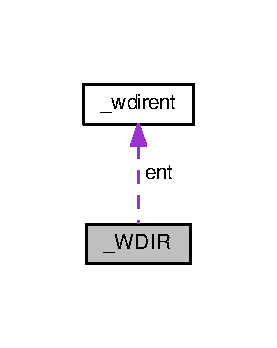
\includegraphics[width=133pt]{struct__WDIR__coll__graph}
\end{center}
\end{figure}
\subsection*{Public Attributes}
\begin{DoxyCompactItemize}
\item 
struct \hyperlink{struct__wdirent}{\+\_\+wdirent} {\bfseries ent}\hypertarget{struct__WDIR_a84ae1457352005f813ed4b3dc1994b62}{}\label{struct__WDIR_a84ae1457352005f813ed4b3dc1994b62}

\item 
W\+I\+N32\+\_\+\+F\+I\+N\+D\+\_\+\+D\+A\+T\+AW {\bfseries data}\hypertarget{struct__WDIR_a065b17b666ee06c4e8068d8accb0eef9}{}\label{struct__WDIR_a065b17b666ee06c4e8068d8accb0eef9}

\item 
int {\bfseries cached}\hypertarget{struct__WDIR_a9b7432df163d1e291ba5925347fd4af3}{}\label{struct__WDIR_a9b7432df163d1e291ba5925347fd4af3}

\item 
H\+A\+N\+D\+LE {\bfseries handle}\hypertarget{struct__WDIR_a694510e166fd3e797b3e15b9e4b3810a}{}\label{struct__WDIR_a694510e166fd3e797b3e15b9e4b3810a}

\item 
wchar\+\_\+t $\ast$ {\bfseries patt}\hypertarget{struct__WDIR_a700ff3a1096fb36452c571b0f55b4e60}{}\label{struct__WDIR_a700ff3a1096fb36452c571b0f55b4e60}

\end{DoxyCompactItemize}


The documentation for this struct was generated from the following file\+:\begin{DoxyCompactItemize}
\item 
Source/\+G\+\_\+\+System/direntw.\+h\end{DoxyCompactItemize}

\hypertarget{struct__wdirent}{}\section{\+\_\+wdirent Struct Reference}
\label{struct__wdirent}\index{\+\_\+wdirent@{\+\_\+wdirent}}
\subsection*{Public Attributes}
\begin{DoxyCompactItemize}
\item 
long {\bfseries d\+\_\+ino}\hypertarget{struct__wdirent_ac8cfaf294a0b6a49287d3f384c280c93}{}\label{struct__wdirent_ac8cfaf294a0b6a49287d3f384c280c93}

\item 
unsigned short {\bfseries d\+\_\+reclen}\hypertarget{struct__wdirent_aff7f360608e576cd18cf11f2caf13ef3}{}\label{struct__wdirent_aff7f360608e576cd18cf11f2caf13ef3}

\item 
size\+\_\+t {\bfseries d\+\_\+namlen}\hypertarget{struct__wdirent_a0050d6131e6fa90206903e216b38799e}{}\label{struct__wdirent_a0050d6131e6fa90206903e216b38799e}

\item 
int {\bfseries d\+\_\+type}\hypertarget{struct__wdirent_a3c3874604ffccbeeaffd96709763cc3b}{}\label{struct__wdirent_a3c3874604ffccbeeaffd96709763cc3b}

\item 
wchar\+\_\+t {\bfseries d\+\_\+name} \mbox{[}P\+A\+T\+H\+\_\+\+M\+AX\mbox{]}\hypertarget{struct__wdirent_a267f915cd36cad5969337a9192cab567}{}\label{struct__wdirent_a267f915cd36cad5969337a9192cab567}

\end{DoxyCompactItemize}


The documentation for this struct was generated from the following file\+:\begin{DoxyCompactItemize}
\item 
Source/\+G\+\_\+\+System/direntw.\+h\end{DoxyCompactItemize}

\hypertarget{classBufferedInput}{}\section{Buffered\+Input Class Reference}
\label{classBufferedInput}\index{Buffered\+Input@{Buffered\+Input}}


Inheritance diagram for Buffered\+Input\+:
\nopagebreak
\begin{figure}[H]
\begin{center}
\leavevmode
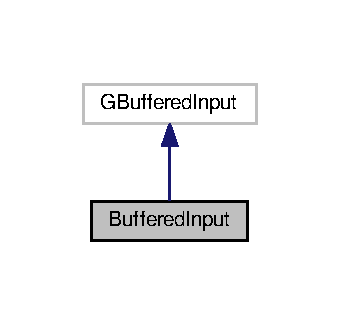
\includegraphics[width=163pt]{classBufferedInput__inherit__graph}
\end{center}
\end{figure}


Collaboration diagram for Buffered\+Input\+:
\nopagebreak
\begin{figure}[H]
\begin{center}
\leavevmode
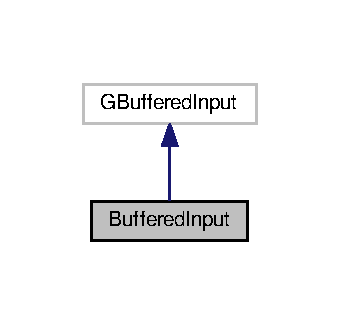
\includegraphics[width=163pt]{classBufferedInput__coll__graph}
\end{center}
\end{figure}
\subsection*{Public Member Functions}
\begin{DoxyCompactItemize}
\item 
void {\bfseries Input\+Thread} ()\hypertarget{classBufferedInput_a198931e0dc2e54a301b016fc51c5f7e5}{}\label{classBufferedInput_a198931e0dc2e54a301b016fc51c5f7e5}

\item 
\hyperlink{namespaceGW_a67a839e3df7ea8a5c5686613a7a3de21}{G\+Return} {\bfseries Initialize\+Windows} (void $\ast$\+\_\+data)\hypertarget{classBufferedInput_ab8594ef04a6bf4100b835c6ff8199d76}{}\label{classBufferedInput_ab8594ef04a6bf4100b835c6ff8199d76}

\item 
\hyperlink{namespaceGW_a67a839e3df7ea8a5c5686613a7a3de21}{G\+Return} {\bfseries Initialize\+Linux} (void $\ast$\+\_\+data)\hypertarget{classBufferedInput_ad82e212f6f9cef33ed3255cae15eaae7}{}\label{classBufferedInput_ad82e212f6f9cef33ed3255cae15eaae7}

\item 
\hyperlink{namespaceGW_a67a839e3df7ea8a5c5686613a7a3de21}{G\+Return} {\bfseries Initialize\+Mac} (void $\ast$\+\_\+data)\hypertarget{classBufferedInput_a18b419bcd05afc3cf306a2f3851d0c0f}{}\label{classBufferedInput_a18b419bcd05afc3cf306a2f3851d0c0f}

\item 
\hyperlink{namespaceGW_a67a839e3df7ea8a5c5686613a7a3de21}{G\+Return} {\bfseries Get\+Count} (unsigned int \&\+\_\+out\+Count)\hypertarget{classBufferedInput_af98a80ccd4b851192264e37aad15c3ab}{}\label{classBufferedInput_af98a80ccd4b851192264e37aad15c3ab}

\item 
\hyperlink{namespaceGW_a67a839e3df7ea8a5c5686613a7a3de21}{G\+Return} {\bfseries Increment\+Count} ()\hypertarget{classBufferedInput_a022aa95811f5426fe68ba04bbbefb413}{}\label{classBufferedInput_a022aa95811f5426fe68ba04bbbefb413}

\item 
\hyperlink{namespaceGW_a67a839e3df7ea8a5c5686613a7a3de21}{G\+Return} {\bfseries Decrement\+Count} ()\hypertarget{classBufferedInput_a74ca447adf3838cbea5c8e42e440a300}{}\label{classBufferedInput_a74ca447adf3838cbea5c8e42e440a300}

\item 
\hyperlink{namespaceGW_a67a839e3df7ea8a5c5686613a7a3de21}{G\+Return} {\bfseries Request\+Interface} (const \hyperlink{structGW_1_1GUUIID}{G\+U\+U\+I\+ID} \&\+\_\+interface\+ID, void $\ast$$\ast$\+\_\+output\+Interface)\hypertarget{classBufferedInput_a31065a70d0fb3fca9f458e7dd25c5df7}{}\label{classBufferedInput_a31065a70d0fb3fca9f458e7dd25c5df7}

\item 
\hyperlink{namespaceGW_a67a839e3df7ea8a5c5686613a7a3de21}{G\+Return} {\bfseries Register\+Listener} (\hyperlink{classGW_1_1CORE_1_1GListener}{G\+Listener} $\ast$\+\_\+add\+Listener, unsigned long long \+\_\+event\+Mask)\hypertarget{classBufferedInput_a210c1c6357ea98ed6cb443fc9e834dca}{}\label{classBufferedInput_a210c1c6357ea98ed6cb443fc9e834dca}

\item 
\hyperlink{namespaceGW_a67a839e3df7ea8a5c5686613a7a3de21}{G\+Return} {\bfseries Deregister\+Listener} (\hyperlink{classGW_1_1CORE_1_1GListener}{G\+Listener} $\ast$\+\_\+remove\+Listener)\hypertarget{classBufferedInput_ac3b002049f7542f8d6e2d87e29113f8c}{}\label{classBufferedInput_ac3b002049f7542f8d6e2d87e29113f8c}

\end{DoxyCompactItemize}


The documentation for this class was generated from the following file\+:\begin{DoxyCompactItemize}
\item 
Source/\+G\+\_\+\+System/G\+Buffered\+Input.\+cpp\end{DoxyCompactItemize}

\hypertarget{structDIR}{}\section{D\+IR Struct Reference}
\label{structDIR}\index{D\+IR@{D\+IR}}


Collaboration diagram for D\+IR\+:\nopagebreak
\begin{figure}[H]
\begin{center}
\leavevmode
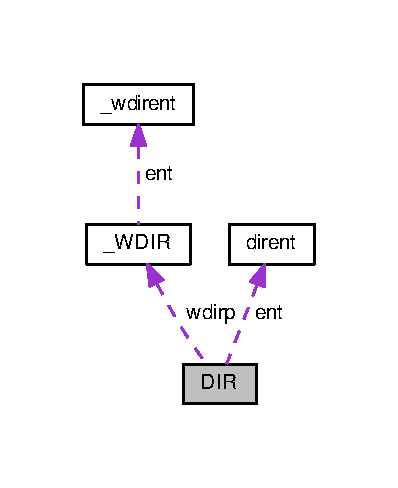
\includegraphics[width=191pt]{structDIR__coll__graph}
\end{center}
\end{figure}
\subsection*{Public Attributes}
\begin{DoxyCompactItemize}
\item 
struct \hyperlink{structdirent}{dirent} {\bfseries ent}\hypertarget{structDIR_a59e9f5211cbb2f8e5b2807ccfdd2a7fc}{}\label{structDIR_a59e9f5211cbb2f8e5b2807ccfdd2a7fc}

\item 
struct \hyperlink{struct__WDIR}{\+\_\+\+W\+D\+IR} $\ast$ {\bfseries wdirp}\hypertarget{structDIR_a29362d4a3d7f809d0f5418b26cac5d41}{}\label{structDIR_a29362d4a3d7f809d0f5418b26cac5d41}

\end{DoxyCompactItemize}


The documentation for this struct was generated from the following file\+:\begin{DoxyCompactItemize}
\item 
Source/\+G\+\_\+\+System/direntw.\+h\end{DoxyCompactItemize}

\hypertarget{structdirent}{}\section{dirent Struct Reference}
\label{structdirent}\index{dirent@{dirent}}
\subsection*{Public Attributes}
\begin{DoxyCompactItemize}
\item 
long {\bfseries d\+\_\+ino}\hypertarget{structdirent_acb6fecfb0e0f6fdc226dff8d56c3da4a}{}\label{structdirent_acb6fecfb0e0f6fdc226dff8d56c3da4a}

\item 
unsigned short {\bfseries d\+\_\+reclen}\hypertarget{structdirent_a90dc47836e8ef510437317876368859e}{}\label{structdirent_a90dc47836e8ef510437317876368859e}

\item 
size\+\_\+t {\bfseries d\+\_\+namlen}\hypertarget{structdirent_a09ced068b03cdb339e34840c8b709621}{}\label{structdirent_a09ced068b03cdb339e34840c8b709621}

\item 
int {\bfseries d\+\_\+type}\hypertarget{structdirent_ad6a736cb04c7295e8f97f708324b3500}{}\label{structdirent_ad6a736cb04c7295e8f97f708324b3500}

\item 
char {\bfseries d\+\_\+name} \mbox{[}P\+A\+T\+H\+\_\+\+M\+AX\mbox{]}\hypertarget{structdirent_a6c68ac080755453ec52de202e91de59b}{}\label{structdirent_a6c68ac080755453ec52de202e91de59b}

\end{DoxyCompactItemize}


The documentation for this struct was generated from the following file\+:\begin{DoxyCompactItemize}
\item 
Source/\+G\+\_\+\+System/direntw.\+h\end{DoxyCompactItemize}

\hypertarget{classFileIO}{}\section{File\+IO Class Reference}
\label{classFileIO}\index{File\+IO@{File\+IO}}


Inheritance diagram for File\+IO\+:\nopagebreak
\begin{figure}[H]
\begin{center}
\leavevmode
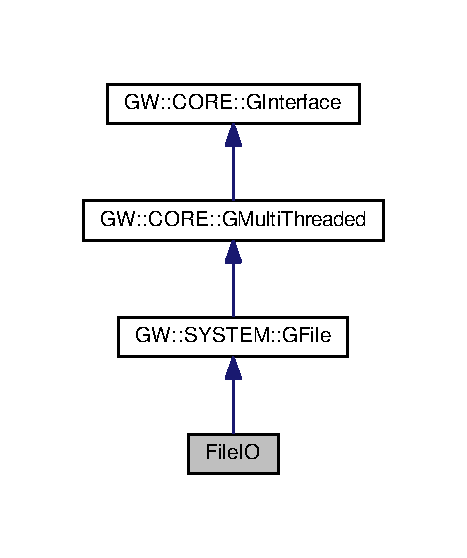
\includegraphics[width=224pt]{classFileIO__inherit__graph}
\end{center}
\end{figure}


Collaboration diagram for File\+IO\+:\nopagebreak
\begin{figure}[H]
\begin{center}
\leavevmode
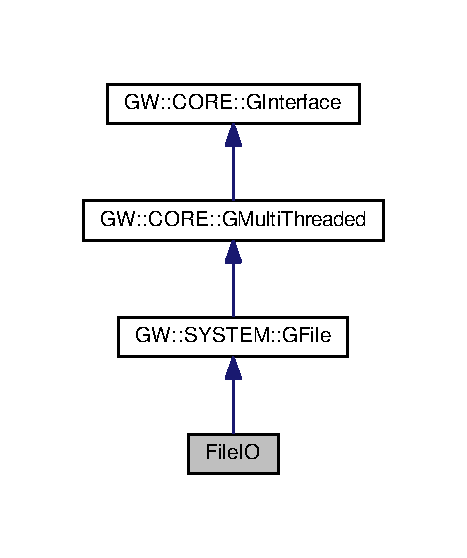
\includegraphics[width=224pt]{classFileIO__coll__graph}
\end{center}
\end{figure}
\subsection*{Public Member Functions}
\begin{DoxyCompactItemize}
\item 
\hyperlink{namespaceGW_a67a839e3df7ea8a5c5686613a7a3de21}{G\+W\+::\+G\+Return} \hyperlink{classFileIO_a0adeb88dd23bb5897e8315ab0029c835}{Open\+Binary\+Read} (const char $\ast$const \+\_\+file) override
\begin{DoxyCompactList}\small\item\em Opens a file for binary read. \end{DoxyCompactList}\item 
\hyperlink{namespaceGW_a67a839e3df7ea8a5c5686613a7a3de21}{G\+W\+::\+G\+Return} \hyperlink{classFileIO_a5cd87c21a72ae2dba21a9f3e50841e6e}{Open\+Binary\+Write} (const char $\ast$const \+\_\+file) override
\begin{DoxyCompactList}\small\item\em Opens a file for binary write with truncation. \end{DoxyCompactList}\item 
\hyperlink{namespaceGW_a67a839e3df7ea8a5c5686613a7a3de21}{G\+W\+::\+G\+Return} \hyperlink{classFileIO_ab26fc846b30446edf28ac922759c9e5e}{Append\+Binary\+Write} (const char $\ast$const \+\_\+file) override
\begin{DoxyCompactList}\small\item\em Opens a file for binary write with append. \end{DoxyCompactList}\item 
\hyperlink{namespaceGW_a67a839e3df7ea8a5c5686613a7a3de21}{G\+W\+::\+G\+Return} \hyperlink{classFileIO_a3d93902abce1baec299cd63891798681}{Open\+Text\+Read} (const char $\ast$const \+\_\+file) override
\begin{DoxyCompactList}\small\item\em Opens a file for text read. \end{DoxyCompactList}\item 
\hyperlink{namespaceGW_a67a839e3df7ea8a5c5686613a7a3de21}{G\+W\+::\+G\+Return} \hyperlink{classFileIO_a4e51443206e9cf97dcac28719dbeb23e}{Open\+Text\+Write} (const char $\ast$const \+\_\+file) override
\begin{DoxyCompactList}\small\item\em Opens a file for text write with truncation. \end{DoxyCompactList}\item 
\hyperlink{namespaceGW_a67a839e3df7ea8a5c5686613a7a3de21}{G\+W\+::\+G\+Return} \hyperlink{classFileIO_afd4e0d14b85d8c0aded66bd946c291f4}{Append\+Text\+Write} (const char $\ast$const \+\_\+file) override
\begin{DoxyCompactList}\small\item\em Opens a file for text write with append. \end{DoxyCompactList}\item 
\hyperlink{namespaceGW_a67a839e3df7ea8a5c5686613a7a3de21}{G\+W\+::\+G\+Return} \hyperlink{classFileIO_a6d849348b4255304b9a1c0c2bd4cd231}{Write} (const char $\ast$const \+\_\+in\+Data, unsigned int \+\_\+num\+Bytes) override
\begin{DoxyCompactList}\small\item\em Writes binary data to the currently opened file. \end{DoxyCompactList}\item 
\hyperlink{namespaceGW_a67a839e3df7ea8a5c5686613a7a3de21}{G\+W\+::\+G\+Return} \hyperlink{classFileIO_adb5270ace70c0189525a7c21c5be31b9}{Read} (char $\ast$\+\_\+out\+Data, unsigned int \+\_\+num\+Bytes) override
\begin{DoxyCompactList}\small\item\em Reads binary from the currently opened file. \end{DoxyCompactList}\item 
\hyperlink{namespaceGW_a67a839e3df7ea8a5c5686613a7a3de21}{G\+W\+::\+G\+Return} \hyperlink{classFileIO_af76c68078333756f887d7298fe9c3492}{Write\+Line} (const char $\ast$const \+\_\+in\+Data) override
\begin{DoxyCompactList}\small\item\em Writes text to the currently opened file. \end{DoxyCompactList}\item 
\hyperlink{namespaceGW_a67a839e3df7ea8a5c5686613a7a3de21}{G\+W\+::\+G\+Return} \hyperlink{classFileIO_a2178a711eb984539cefe6d651a7167fb}{Read\+Line} (char $\ast$\+\_\+out\+Data, unsigned int \+\_\+out\+Data\+Size, char \+\_\+delimiter) override
\begin{DoxyCompactList}\small\item\em Reads text to the currently opened file. \end{DoxyCompactList}\item 
\hyperlink{namespaceGW_a67a839e3df7ea8a5c5686613a7a3de21}{G\+W\+::\+G\+Return} \hyperlink{classFileIO_a906610c8653ba8ca476dc46679851590}{Close\+File} () override
\begin{DoxyCompactList}\small\item\em Flushes and closes the current file. \end{DoxyCompactList}\item 
\hyperlink{namespaceGW_a67a839e3df7ea8a5c5686613a7a3de21}{G\+W\+::\+G\+Return} \hyperlink{classFileIO_a8e5afdb1a734f37e422ff0147561a3a1}{Flush\+File} () override
\begin{DoxyCompactList}\small\item\em Flushes the current file. \end{DoxyCompactList}\item 
\hyperlink{namespaceGW_a67a839e3df7ea8a5c5686613a7a3de21}{G\+W\+::\+G\+Return} \hyperlink{classFileIO_a8332ededccf4034fd83509d9513a2635}{Set\+Current\+Working\+Directory} (const char $\ast$const \+\_\+dir) override
\begin{DoxyCompactList}\small\item\em Changes the current working directory. \end{DoxyCompactList}\item 
\hyperlink{namespaceGW_a67a839e3df7ea8a5c5686613a7a3de21}{G\+W\+::\+G\+Return} \hyperlink{classFileIO_a41a1859ffe3ebd76005f264af0b1ea66}{Get\+Current\+Working\+Directory} (char $\ast$\+\_\+dir, unsigned int \+\_\+dir\+Size) override
\begin{DoxyCompactList}\small\item\em Retrieves the absolute path of the current working directory. \end{DoxyCompactList}\item 
\hyperlink{namespaceGW_a67a839e3df7ea8a5c5686613a7a3de21}{G\+W\+::\+G\+Return} \hyperlink{classFileIO_ae331f6c02948720d9cc5bcd2700d8cf7}{Get\+Directory\+Size} (unsigned int \&\+\_\+out\+Size) override
\begin{DoxyCompactList}\small\item\em Gets the number of files in the current working directory. \end{DoxyCompactList}\item 
\hyperlink{namespaceGW_a67a839e3df7ea8a5c5686613a7a3de21}{G\+W\+::\+G\+Return} \hyperlink{classFileIO_afd1b77afed3d853aaa01f14ecbc6b0e0}{Get\+Files\+From\+Directory} (char $\ast$\+\_\+out\+Files\mbox{[}$\,$\mbox{]}, unsigned int \+\_\+num\+Files, unsigned int \+\_\+file\+Name\+Size) override
\begin{DoxyCompactList}\small\item\em Gets the names of all files in the current working directory. \end{DoxyCompactList}\item 
\hyperlink{namespaceGW_a67a839e3df7ea8a5c5686613a7a3de21}{G\+W\+::\+G\+Return} \hyperlink{classFileIO_a91ee3ceabd5d6097eed85466c26d2adb}{Get\+File\+Size} (const char $\ast$const \+\_\+file, unsigned int \&\+\_\+out\+Size) override
\begin{DoxyCompactList}\small\item\em Gets the size of the specified file in bytes. \end{DoxyCompactList}\item 
\hyperlink{namespaceGW_a67a839e3df7ea8a5c5686613a7a3de21}{G\+W\+::\+G\+Return} \hyperlink{classFileIO_a20566e320ec4cc0d5615bc3bc1fa3013}{Get\+Count} (unsigned int \&\+\_\+out\+Count) override
\begin{DoxyCompactList}\small\item\em Return the total number of active references to this object. \end{DoxyCompactList}\item 
\hyperlink{namespaceGW_a67a839e3df7ea8a5c5686613a7a3de21}{G\+W\+::\+G\+Return} \hyperlink{classFileIO_a9f2c9a4d13577e14a2c94b0e9617d80b}{Increment\+Count} () override
\begin{DoxyCompactList}\small\item\em Increase the total number of active references to this object. \end{DoxyCompactList}\item 
\hyperlink{namespaceGW_a67a839e3df7ea8a5c5686613a7a3de21}{G\+W\+::\+G\+Return} \hyperlink{classFileIO_ab7e4806ca819c3fcdeeb40a2af5f0298}{Decrement\+Count} () override
\begin{DoxyCompactList}\small\item\em Decrease the total number of active references to this object. \end{DoxyCompactList}\item 
\hyperlink{namespaceGW_a67a839e3df7ea8a5c5686613a7a3de21}{G\+W\+::\+G\+Return} \hyperlink{classFileIO_a3fb39527fac479474c6ef5045dbc1551}{Request\+Interface} (const \hyperlink{structGW_1_1GUUIID}{G\+W\+::\+G\+U\+U\+I\+ID} \&\+\_\+interface\+ID, void $\ast$$\ast$\+\_\+output\+Interface) override
\begin{DoxyCompactList}\small\item\em Requests an interface that may or may not be supported by this object. \end{DoxyCompactList}\item 
\hyperlink{namespaceGW_a67a839e3df7ea8a5c5686613a7a3de21}{G\+W\+::\+G\+Return} {\bfseries Init} ()\hypertarget{classFileIO_a1c24bf6f35d30462fd918e5ee1a44033}{}\label{classFileIO_a1c24bf6f35d30462fd918e5ee1a44033}

\end{DoxyCompactItemize}


\subsection{Member Function Documentation}
\index{File\+IO@{File\+IO}!Append\+Binary\+Write@{Append\+Binary\+Write}}
\index{Append\+Binary\+Write@{Append\+Binary\+Write}!File\+IO@{File\+IO}}
\subsubsection[{\texorpdfstring{Append\+Binary\+Write(const char $\ast$const \+\_\+file) override}{AppendBinaryWrite(const char *const _file) override}}]{\setlength{\rightskip}{0pt plus 5cm}{\bf G\+W\+::\+G\+Return} File\+I\+O\+::\+Append\+Binary\+Write (
\begin{DoxyParamCaption}
\item[{const char $\ast$const}]{\+\_\+file}
\end{DoxyParamCaption}
)\hspace{0.3cm}{\ttfamily [override]}, {\ttfamily [virtual]}}\hypertarget{classFileIO_ab26fc846b30446edf28ac922759c9e5e}{}\label{classFileIO_ab26fc846b30446edf28ac922759c9e5e}


Opens a file for binary write with append. 

The file name passed into the function should be passed like it is a relative path. The function will look in the current working directory for the file. If the file is not found in the current working directory, the file will be created in the current working directory. File can now be written to with \hyperlink{classFileIO_a6d849348b4255304b9a1c0c2bd4cd231}{Write()}.


\begin{DoxyParams}[1]{Parameters}
\mbox{\tt in}  & {\em \+\_\+file} & The file name of the file to open.\\
\hline
\end{DoxyParams}

\begin{DoxyRetVals}{Return values}
{\em S\+U\+C\+C\+E\+SS} & Succesfully opened the file. \\
\hline
{\em F\+A\+I\+L\+U\+RE} & A file is already open or the file could not be found/created. \\
\hline
{\em I\+N\+V\+A\+L\+I\+D\+\_\+\+A\+R\+G\+U\+M\+E\+NT} & A nullptr was passed in. \\
\hline
\end{DoxyRetVals}


Implements \hyperlink{classGW_1_1SYSTEM_1_1GFile_a63311236692181f99fd393fe8e1ca9fc}{G\+W\+::\+S\+Y\+S\+T\+E\+M\+::\+G\+File}.

\index{File\+IO@{File\+IO}!Append\+Text\+Write@{Append\+Text\+Write}}
\index{Append\+Text\+Write@{Append\+Text\+Write}!File\+IO@{File\+IO}}
\subsubsection[{\texorpdfstring{Append\+Text\+Write(const char $\ast$const \+\_\+file) override}{AppendTextWrite(const char *const _file) override}}]{\setlength{\rightskip}{0pt plus 5cm}{\bf G\+W\+::\+G\+Return} File\+I\+O\+::\+Append\+Text\+Write (
\begin{DoxyParamCaption}
\item[{const char $\ast$const}]{\+\_\+file}
\end{DoxyParamCaption}
)\hspace{0.3cm}{\ttfamily [override]}, {\ttfamily [virtual]}}\hypertarget{classFileIO_afd4e0d14b85d8c0aded66bd946c291f4}{}\label{classFileIO_afd4e0d14b85d8c0aded66bd946c291f4}


Opens a file for text write with append. 

The file name passed into the function should be passed like it is a relative path. The function will look in the current working directory for the file. If the file is not found in the current working directory, the file will be created in the current working directory. File can now be written to with \hyperlink{classFileIO_a6d849348b4255304b9a1c0c2bd4cd231}{Write()}.


\begin{DoxyParams}[1]{Parameters}
\mbox{\tt in}  & {\em \+\_\+file} & The file name of the file to open.\\
\hline
\end{DoxyParams}

\begin{DoxyRetVals}{Return values}
{\em S\+U\+C\+C\+E\+SS} & Succesfully opened the file. \\
\hline
{\em F\+A\+I\+L\+U\+RE} & A file is already open or the file could not be found/created. \\
\hline
{\em I\+N\+V\+A\+L\+I\+D\+\_\+\+A\+R\+G\+U\+M\+E\+NT} & A nullptr was passed in. \\
\hline
\end{DoxyRetVals}


Implements \hyperlink{classGW_1_1SYSTEM_1_1GFile_a72e40b3234a2384738d8db6e958f4782}{G\+W\+::\+S\+Y\+S\+T\+E\+M\+::\+G\+File}.

\index{File\+IO@{File\+IO}!Close\+File@{Close\+File}}
\index{Close\+File@{Close\+File}!File\+IO@{File\+IO}}
\subsubsection[{\texorpdfstring{Close\+File() override}{CloseFile() override}}]{\setlength{\rightskip}{0pt plus 5cm}{\bf G\+W\+::\+G\+Return} File\+I\+O\+::\+Close\+File (
\begin{DoxyParamCaption}
{}
\end{DoxyParamCaption}
)\hspace{0.3cm}{\ttfamily [override]}, {\ttfamily [virtual]}}\hypertarget{classFileIO_a906610c8653ba8ca476dc46679851590}{}\label{classFileIO_a906610c8653ba8ca476dc46679851590}


Flushes and closes the current file. 


\begin{DoxyRetVals}{Return values}
{\em S\+U\+C\+C\+E\+SS} & File successfully flushed and closed. \\
\hline
{\em F\+A\+I\+L\+U\+RE} & A file is not currently open. \\
\hline
\end{DoxyRetVals}


Implements \hyperlink{classGW_1_1SYSTEM_1_1GFile_ae661d107c461145bb095dcfc76519f54}{G\+W\+::\+S\+Y\+S\+T\+E\+M\+::\+G\+File}.

\index{File\+IO@{File\+IO}!Decrement\+Count@{Decrement\+Count}}
\index{Decrement\+Count@{Decrement\+Count}!File\+IO@{File\+IO}}
\subsubsection[{\texorpdfstring{Decrement\+Count() override}{DecrementCount() override}}]{\setlength{\rightskip}{0pt plus 5cm}{\bf G\+W\+::\+G\+Return} File\+I\+O\+::\+Decrement\+Count (
\begin{DoxyParamCaption}
{}
\end{DoxyParamCaption}
)\hspace{0.3cm}{\ttfamily [override]}, {\ttfamily [virtual]}}\hypertarget{classFileIO_ab7e4806ca819c3fcdeeb40a2af5f0298}{}\label{classFileIO_ab7e4806ca819c3fcdeeb40a2af5f0298}


Decrease the total number of active references to this object. 

Once the internal count reaches zero this object will be deallocated and your pointer will become invalid.


\begin{DoxyRetVals}{Return values}
{\em S\+U\+C\+C\+E\+SS} & Successfully decremented the internal reference count. \\
\hline
{\em F\+A\+I\+L\+U\+RE} & Decrementing of internal reference count would underflow the value. \\
\hline
\end{DoxyRetVals}


Implements \hyperlink{classGW_1_1CORE_1_1GInterface_a19a368c77ad0aa7f49b5a4f772f173ba}{G\+W\+::\+C\+O\+R\+E\+::\+G\+Interface}.

\index{File\+IO@{File\+IO}!Flush\+File@{Flush\+File}}
\index{Flush\+File@{Flush\+File}!File\+IO@{File\+IO}}
\subsubsection[{\texorpdfstring{Flush\+File() override}{FlushFile() override}}]{\setlength{\rightskip}{0pt plus 5cm}{\bf G\+W\+::\+G\+Return} File\+I\+O\+::\+Flush\+File (
\begin{DoxyParamCaption}
{}
\end{DoxyParamCaption}
)\hspace{0.3cm}{\ttfamily [override]}, {\ttfamily [virtual]}}\hypertarget{classFileIO_a8e5afdb1a734f37e422ff0147561a3a1}{}\label{classFileIO_a8e5afdb1a734f37e422ff0147561a3a1}


Flushes the current file. 


\begin{DoxyRetVals}{Return values}
{\em S\+U\+C\+C\+E\+SS} & File successfully flushed. \\
\hline
{\em F\+A\+I\+L\+U\+RE} & A file is not currently open. \\
\hline
\end{DoxyRetVals}


Implements \hyperlink{classGW_1_1SYSTEM_1_1GFile_ae3105b637ef87af268722a696b8657a9}{G\+W\+::\+S\+Y\+S\+T\+E\+M\+::\+G\+File}.

\index{File\+IO@{File\+IO}!Get\+Count@{Get\+Count}}
\index{Get\+Count@{Get\+Count}!File\+IO@{File\+IO}}
\subsubsection[{\texorpdfstring{Get\+Count(unsigned int \&\+\_\+out\+Count) override}{GetCount(unsigned int &_outCount) override}}]{\setlength{\rightskip}{0pt plus 5cm}{\bf G\+W\+::\+G\+Return} File\+I\+O\+::\+Get\+Count (
\begin{DoxyParamCaption}
\item[{unsigned int \&}]{\+\_\+out\+Count}
\end{DoxyParamCaption}
)\hspace{0.3cm}{\ttfamily [override]}, {\ttfamily [virtual]}}\hypertarget{classFileIO_a20566e320ec4cc0d5615bc3bc1fa3013}{}\label{classFileIO_a20566e320ec4cc0d5615bc3bc1fa3013}


Return the total number of active references to this object. 


\begin{DoxyParams}[1]{Parameters}
\mbox{\tt out}  & {\em \+\_\+out\+Count} & The total number of active references of this object.\\
\hline
\end{DoxyParams}

\begin{DoxyRetVals}{Return values}
{\em S\+U\+C\+C\+E\+SS} & Successfully ran. \\
\hline
{\em F\+A\+I\+L\+U\+RE} & Either class does not exist or the internal reference count is corrupt. \\
\hline
\end{DoxyRetVals}


Implements \hyperlink{classGW_1_1CORE_1_1GInterface_aacf5834174a7024f8a3c361122ee9e76}{G\+W\+::\+C\+O\+R\+E\+::\+G\+Interface}.

\index{File\+IO@{File\+IO}!Get\+Current\+Working\+Directory@{Get\+Current\+Working\+Directory}}
\index{Get\+Current\+Working\+Directory@{Get\+Current\+Working\+Directory}!File\+IO@{File\+IO}}
\subsubsection[{\texorpdfstring{Get\+Current\+Working\+Directory(char $\ast$\+\_\+dir, unsigned int \+\_\+dir\+Size) override}{GetCurrentWorkingDirectory(char *_dir, unsigned int _dirSize) override}}]{\setlength{\rightskip}{0pt plus 5cm}{\bf G\+W\+::\+G\+Return} File\+I\+O\+::\+Get\+Current\+Working\+Directory (
\begin{DoxyParamCaption}
\item[{char $\ast$}]{\+\_\+out\+Dir, }
\item[{unsigned int}]{\+\_\+dir\+Size}
\end{DoxyParamCaption}
)\hspace{0.3cm}{\ttfamily [override]}, {\ttfamily [virtual]}}\hypertarget{classFileIO_a41a1859ffe3ebd76005f264af0b1ea66}{}\label{classFileIO_a41a1859ffe3ebd76005f264af0b1ea66}


Retrieves the absolute path of the current working directory. 

This is the directory we will look into for any file Open commands. This is by Windows standard guaranteed to be 255 or less.


\begin{DoxyParams}[1]{Parameters}
\mbox{\tt out}  & {\em \+\_\+out\+Dir} & An absolute path to the directory to set as the current working directory. \\
\hline
\mbox{\tt in}  & {\em \+\_\+dir\+Size} & The size of \+\_\+out\+Dir.\\
\hline
\end{DoxyParams}

\begin{DoxyRetVals}{Return values}
{\em S\+U\+C\+C\+E\+SS} & Successfully obtained the working directory. \\
\hline
{\em F\+A\+I\+L\+U\+RE} & The current working directory is invalid or \+\_\+out\+Dir was not big enough. \+\_\+out\+Dir will be null. \\
\hline
{\em I\+N\+V\+A\+L\+I\+D\+\_\+\+A\+R\+G\+U\+M\+E\+NT} & A nullptr was passed in or the size is 0. \\
\hline
\end{DoxyRetVals}


Implements \hyperlink{classGW_1_1SYSTEM_1_1GFile_a6853b717e838d1b3a54f22449a37d764}{G\+W\+::\+S\+Y\+S\+T\+E\+M\+::\+G\+File}.

\index{File\+IO@{File\+IO}!Get\+Directory\+Size@{Get\+Directory\+Size}}
\index{Get\+Directory\+Size@{Get\+Directory\+Size}!File\+IO@{File\+IO}}
\subsubsection[{\texorpdfstring{Get\+Directory\+Size(unsigned int \&\+\_\+out\+Size) override}{GetDirectorySize(unsigned int &_outSize) override}}]{\setlength{\rightskip}{0pt plus 5cm}{\bf G\+W\+::\+G\+Return} File\+I\+O\+::\+Get\+Directory\+Size (
\begin{DoxyParamCaption}
\item[{unsigned int \&}]{\+\_\+out\+Size}
\end{DoxyParamCaption}
)\hspace{0.3cm}{\ttfamily [override]}, {\ttfamily [virtual]}}\hypertarget{classFileIO_ae331f6c02948720d9cc5bcd2700d8cf7}{}\label{classFileIO_ae331f6c02948720d9cc5bcd2700d8cf7}


Gets the number of files in the current working directory. 


\begin{DoxyParams}[1]{Parameters}
\mbox{\tt out}  & {\em \+\_\+out\+Size} & The number of files in the directory.\\
\hline
\end{DoxyParams}

\begin{DoxyRetVals}{Return values}
{\em S\+U\+C\+C\+E\+SS} & Successfully counted the files in the directory. \\
\hline
{\em F\+A\+I\+L\+U\+RE} & Either currently working directory is invalid or count failed. \+\_\+out\+Size will be -\/1. \\
\hline
\end{DoxyRetVals}


Implements \hyperlink{classGW_1_1SYSTEM_1_1GFile_ac2de86bf6cf61455577efc47277ecb94}{G\+W\+::\+S\+Y\+S\+T\+E\+M\+::\+G\+File}.

\index{File\+IO@{File\+IO}!Get\+Files\+From\+Directory@{Get\+Files\+From\+Directory}}
\index{Get\+Files\+From\+Directory@{Get\+Files\+From\+Directory}!File\+IO@{File\+IO}}
\subsubsection[{\texorpdfstring{Get\+Files\+From\+Directory(char $\ast$\+\_\+out\+Files[], unsigned int \+\_\+num\+Files, unsigned int \+\_\+file\+Name\+Size) override}{GetFilesFromDirectory(char *_outFiles[], unsigned int _numFiles, unsigned int _fileNameSize) override}}]{\setlength{\rightskip}{0pt plus 5cm}{\bf G\+W\+::\+G\+Return} File\+I\+O\+::\+Get\+Files\+From\+Directory (
\begin{DoxyParamCaption}
\item[{char $\ast$}]{\+\_\+out\+Files\mbox{[}$\,$\mbox{]}, }
\item[{unsigned int}]{\+\_\+num\+Files, }
\item[{unsigned int}]{\+\_\+file\+Name\+Size}
\end{DoxyParamCaption}
)\hspace{0.3cm}{\ttfamily [override]}, {\ttfamily [virtual]}}\hypertarget{classFileIO_afd1b77afed3d853aaa01f14ecbc6b0e0}{}\label{classFileIO_afd1b77afed3d853aaa01f14ecbc6b0e0}


Gets the names of all files in the current working directory. 

This function will retrieve just the file names and extensions. Any Open function using these names will assume the files are in the current working directory. Any change of the current working directory will make these names invalid until called again.


\begin{DoxyParams}[1]{Parameters}
\mbox{\tt out}  & {\em \+\_\+out\+Files} & Stores the names of the files retrieved. \\
\hline
\mbox{\tt in}  & {\em \+\_\+num\+Files} & The number of files. \\
\hline
\mbox{\tt in}  & {\em \+\_\+file\+Name\+Size} & The size of the file names.\\
\hline
\end{DoxyParams}

\begin{DoxyRetVals}{Return values}
{\em S\+U\+C\+C\+E\+SS} & Successfully retrieved the file names. \\
\hline
{\em F\+A\+I\+L\+U\+RE} & Either current working directory is invalid or obtaining file names failed. \\
\hline
\end{DoxyRetVals}


Implements \hyperlink{classGW_1_1SYSTEM_1_1GFile_ae062d19f84d120adea94756d1d26e41e}{G\+W\+::\+S\+Y\+S\+T\+E\+M\+::\+G\+File}.

\index{File\+IO@{File\+IO}!Get\+File\+Size@{Get\+File\+Size}}
\index{Get\+File\+Size@{Get\+File\+Size}!File\+IO@{File\+IO}}
\subsubsection[{\texorpdfstring{Get\+File\+Size(const char $\ast$const \+\_\+file, unsigned int \&\+\_\+out\+Size) override}{GetFileSize(const char *const _file, unsigned int &_outSize) override}}]{\setlength{\rightskip}{0pt plus 5cm}{\bf G\+W\+::\+G\+Return} File\+I\+O\+::\+Get\+File\+Size (
\begin{DoxyParamCaption}
\item[{const char $\ast$const}]{\+\_\+file, }
\item[{unsigned int \&}]{\+\_\+out\+Size}
\end{DoxyParamCaption}
)\hspace{0.3cm}{\ttfamily [override]}, {\ttfamily [virtual]}}\hypertarget{classFileIO_a91ee3ceabd5d6097eed85466c26d2adb}{}\label{classFileIO_a91ee3ceabd5d6097eed85466c26d2adb}


Gets the size of the specified file in bytes. 

The filename passed into this function should be passed as a relative path. This function will assume the file passed in is in the current working directory and will look for it there.


\begin{DoxyParams}[1]{Parameters}
\mbox{\tt in}  & {\em \+\_\+file} & The file to get the size of. \\
\hline
\mbox{\tt out}  & {\em \+\_\+out\+Size} & will store the size of the file.\\
\hline
\end{DoxyParams}

\begin{DoxyRetVals}{Return values}
{\em S\+U\+C\+C\+E\+SS} & Successfully retrieved the file size. \\
\hline
{\em F\+I\+L\+E\+\_\+\+N\+O\+T\+\_\+\+F\+O\+U\+ND} & Could not locate the file. Check that the current working directory is valid. \\
\hline
\end{DoxyRetVals}


Implements \hyperlink{classGW_1_1SYSTEM_1_1GFile_a2f4cba2dad96fa4c894545f43fee64b5}{G\+W\+::\+S\+Y\+S\+T\+E\+M\+::\+G\+File}.

\index{File\+IO@{File\+IO}!Increment\+Count@{Increment\+Count}}
\index{Increment\+Count@{Increment\+Count}!File\+IO@{File\+IO}}
\subsubsection[{\texorpdfstring{Increment\+Count() override}{IncrementCount() override}}]{\setlength{\rightskip}{0pt plus 5cm}{\bf G\+W\+::\+G\+Return} File\+I\+O\+::\+Increment\+Count (
\begin{DoxyParamCaption}
{}
\end{DoxyParamCaption}
)\hspace{0.3cm}{\ttfamily [override]}, {\ttfamily [virtual]}}\hypertarget{classFileIO_a9f2c9a4d13577e14a2c94b0e9617d80b}{}\label{classFileIO_a9f2c9a4d13577e14a2c94b0e9617d80b}


Increase the total number of active references to this object. 

End users should only call this operation if they are familiar with reference counting behavior.


\begin{DoxyRetVals}{Return values}
{\em S\+U\+C\+C\+E\+SS} & Successfully incremented the internal reference count. \\
\hline
{\em F\+A\+I\+L\+U\+RE} & Incrementation of internal reference count would overflow the value. \\
\hline
\end{DoxyRetVals}


Implements \hyperlink{classGW_1_1CORE_1_1GInterface_a2d710f20bb78e544e8309b5b75c21260}{G\+W\+::\+C\+O\+R\+E\+::\+G\+Interface}.

\index{File\+IO@{File\+IO}!Open\+Binary\+Read@{Open\+Binary\+Read}}
\index{Open\+Binary\+Read@{Open\+Binary\+Read}!File\+IO@{File\+IO}}
\subsubsection[{\texorpdfstring{Open\+Binary\+Read(const char $\ast$const \+\_\+file) override}{OpenBinaryRead(const char *const _file) override}}]{\setlength{\rightskip}{0pt plus 5cm}{\bf G\+W\+::\+G\+Return} File\+I\+O\+::\+Open\+Binary\+Read (
\begin{DoxyParamCaption}
\item[{const char $\ast$const}]{\+\_\+file}
\end{DoxyParamCaption}
)\hspace{0.3cm}{\ttfamily [override]}, {\ttfamily [virtual]}}\hypertarget{classFileIO_a0adeb88dd23bb5897e8315ab0029c835}{}\label{classFileIO_a0adeb88dd23bb5897e8315ab0029c835}


Opens a file for binary read. 

The file name passed into the function should be passed like it is a relative path. The function will look in the current working directory for the file. If the file is not found in the current working directory, the function will fail.


\begin{DoxyParams}[1]{Parameters}
\mbox{\tt in}  & {\em \+\_\+file} & The file name of the file to open.\\
\hline
\end{DoxyParams}

\begin{DoxyRetVals}{Return values}
{\em S\+U\+C\+C\+E\+SS} & Succesfully opened the file. \\
\hline
{\em F\+I\+L\+E\+\_\+\+N\+O\+T\+\_\+\+F\+O\+U\+ND} & File could not be found. \\
\hline
{\em F\+A\+I\+L\+U\+RE} & A file is already opened. \\
\hline
{\em I\+N\+V\+A\+L\+I\+D\+\_\+\+A\+R\+G\+U\+M\+E\+NT} & A null pointer was passed in. \\
\hline
\end{DoxyRetVals}


Implements \hyperlink{classGW_1_1SYSTEM_1_1GFile_a2744359d5d258b1b59d139101c6809ce}{G\+W\+::\+S\+Y\+S\+T\+E\+M\+::\+G\+File}.

\index{File\+IO@{File\+IO}!Open\+Binary\+Write@{Open\+Binary\+Write}}
\index{Open\+Binary\+Write@{Open\+Binary\+Write}!File\+IO@{File\+IO}}
\subsubsection[{\texorpdfstring{Open\+Binary\+Write(const char $\ast$const \+\_\+file) override}{OpenBinaryWrite(const char *const _file) override}}]{\setlength{\rightskip}{0pt plus 5cm}{\bf G\+W\+::\+G\+Return} File\+I\+O\+::\+Open\+Binary\+Write (
\begin{DoxyParamCaption}
\item[{const char $\ast$const}]{\+\_\+file}
\end{DoxyParamCaption}
)\hspace{0.3cm}{\ttfamily [override]}, {\ttfamily [virtual]}}\hypertarget{classFileIO_a5cd87c21a72ae2dba21a9f3e50841e6e}{}\label{classFileIO_a5cd87c21a72ae2dba21a9f3e50841e6e}


Opens a file for binary write with truncation. 

The file name passed into the function should be passed like it is a relative path. The function will look in the current working directory for the file. If the file is not found in the current working directory, the file will be created in the current working directory. File can now be read from with \hyperlink{classFileIO_adb5270ace70c0189525a7c21c5be31b9}{Read()}.


\begin{DoxyParams}[1]{Parameters}
\mbox{\tt in}  & {\em \+\_\+file} & The file name of the file to open.\\
\hline
\end{DoxyParams}

\begin{DoxyRetVals}{Return values}
{\em S\+U\+C\+C\+E\+SS} & Succesfully opened the file. \\
\hline
{\em F\+A\+I\+L\+U\+RE} & A file is already open or file could not be found/created. \\
\hline
{\em I\+N\+V\+A\+L\+I\+D\+\_\+\+A\+R\+G\+U\+M\+E\+NT} & A nullptr was passed in. \\
\hline
\end{DoxyRetVals}


Implements \hyperlink{classGW_1_1SYSTEM_1_1GFile_a8d5f335bbc6f7c6d798ed27718aa2347}{G\+W\+::\+S\+Y\+S\+T\+E\+M\+::\+G\+File}.

\index{File\+IO@{File\+IO}!Open\+Text\+Read@{Open\+Text\+Read}}
\index{Open\+Text\+Read@{Open\+Text\+Read}!File\+IO@{File\+IO}}
\subsubsection[{\texorpdfstring{Open\+Text\+Read(const char $\ast$const \+\_\+file) override}{OpenTextRead(const char *const _file) override}}]{\setlength{\rightskip}{0pt plus 5cm}{\bf G\+W\+::\+G\+Return} File\+I\+O\+::\+Open\+Text\+Read (
\begin{DoxyParamCaption}
\item[{const char $\ast$const}]{\+\_\+file}
\end{DoxyParamCaption}
)\hspace{0.3cm}{\ttfamily [override]}, {\ttfamily [virtual]}}\hypertarget{classFileIO_a3d93902abce1baec299cd63891798681}{}\label{classFileIO_a3d93902abce1baec299cd63891798681}


Opens a file for text read. 

The file name passed into the function should be passed like it is a relative path. The function will look in the current working directory for the file. If the file is not found in the current working directory, the function will fail. File can now be written to with \hyperlink{classFileIO_a6d849348b4255304b9a1c0c2bd4cd231}{Write()}.


\begin{DoxyParams}[1]{Parameters}
\mbox{\tt in}  & {\em \+\_\+file} & The file name of the file to open.\\
\hline
\end{DoxyParams}

\begin{DoxyRetVals}{Return values}
{\em S\+U\+C\+C\+E\+SS} & Succesfully opened the file. \\
\hline
{\em F\+I\+L\+E\+\_\+\+N\+O\+T\+\_\+\+F\+O\+U\+ND} & File could not be found. \\
\hline
{\em F\+A\+I\+L\+U\+RE} & A file is already open. \\
\hline
{\em I\+N\+V\+A\+L\+I\+D\+\_\+\+A\+R\+G\+U\+M\+E\+NT} & A nullptr was passed in. \\
\hline
\end{DoxyRetVals}


Implements \hyperlink{classGW_1_1SYSTEM_1_1GFile_ac3ece72ce30e4d1a1c426c53a7a8354a}{G\+W\+::\+S\+Y\+S\+T\+E\+M\+::\+G\+File}.

\index{File\+IO@{File\+IO}!Open\+Text\+Write@{Open\+Text\+Write}}
\index{Open\+Text\+Write@{Open\+Text\+Write}!File\+IO@{File\+IO}}
\subsubsection[{\texorpdfstring{Open\+Text\+Write(const char $\ast$const \+\_\+file) override}{OpenTextWrite(const char *const _file) override}}]{\setlength{\rightskip}{0pt plus 5cm}{\bf G\+W\+::\+G\+Return} File\+I\+O\+::\+Open\+Text\+Write (
\begin{DoxyParamCaption}
\item[{const char $\ast$const}]{\+\_\+file}
\end{DoxyParamCaption}
)\hspace{0.3cm}{\ttfamily [override]}, {\ttfamily [virtual]}}\hypertarget{classFileIO_a4e51443206e9cf97dcac28719dbeb23e}{}\label{classFileIO_a4e51443206e9cf97dcac28719dbeb23e}


Opens a file for text write with truncation. 

The file name passed into the function should be passed like it is a relative path. The function will look in the current working directory for the file. If the file is not found in the current working directory, the file will be created in the current working directory. File can now be read from with \hyperlink{classFileIO_adb5270ace70c0189525a7c21c5be31b9}{Read()}.


\begin{DoxyParams}[1]{Parameters}
\mbox{\tt in}  & {\em \+\_\+file} & The file name of the file to open.\\
\hline
\end{DoxyParams}

\begin{DoxyRetVals}{Return values}
{\em S\+U\+C\+C\+E\+SS} & Succesfully opened the file. \\
\hline
{\em F\+A\+I\+L\+U\+RE} & A file is already open or the file could not be found/created. \\
\hline
{\em I\+N\+V\+A\+L\+I\+D\+\_\+\+A\+R\+G\+U\+M\+E\+NT} & A nullptr was passed in. \\
\hline
\end{DoxyRetVals}


Implements \hyperlink{classGW_1_1SYSTEM_1_1GFile_aebd3e32736b994c0296b7575ab0a2759}{G\+W\+::\+S\+Y\+S\+T\+E\+M\+::\+G\+File}.

\index{File\+IO@{File\+IO}!Read@{Read}}
\index{Read@{Read}!File\+IO@{File\+IO}}
\subsubsection[{\texorpdfstring{Read(char $\ast$\+\_\+out\+Data, unsigned int \+\_\+num\+Bytes) override}{Read(char *_outData, unsigned int _numBytes) override}}]{\setlength{\rightskip}{0pt plus 5cm}{\bf G\+W\+::\+G\+Return} File\+I\+O\+::\+Read (
\begin{DoxyParamCaption}
\item[{char $\ast$}]{\+\_\+out\+Data, }
\item[{unsigned int}]{\+\_\+num\+Bytes}
\end{DoxyParamCaption}
)\hspace{0.3cm}{\ttfamily [override]}, {\ttfamily [virtual]}}\hypertarget{classFileIO_adb5270ace70c0189525a7c21c5be31b9}{}\label{classFileIO_adb5270ace70c0189525a7c21c5be31b9}


Reads binary from the currently opened file. 

Reads binary data and stores it into a char$\ast$ until the byte limit is reached.


\begin{DoxyParams}[1]{Parameters}
\mbox{\tt out}  & {\em \+\_\+out\+Data} & The variable to store the read in bytes. \\
\hline
\mbox{\tt in}  & {\em \+\_\+num\+Bytes} & The number of bytes to read in from the file.\\
\hline
\end{DoxyParams}

\begin{DoxyRetVals}{Return values}
{\em S\+U\+C\+C\+E\+SS} & Successful read. \\
\hline
{\em F\+A\+I\+L\+U\+RE} & Either file is not open or read failed. \+\_\+out\+Data will be null. \\
\hline
{\em I\+N\+V\+A\+L\+I\+D\+\_\+\+A\+R\+G\+U\+M\+E\+NT} & A byte size of 0 was passed in. \\
\hline
\end{DoxyRetVals}


Implements \hyperlink{classGW_1_1SYSTEM_1_1GFile_a1aaa026cba3d37abaaa2b408cd5d322d}{G\+W\+::\+S\+Y\+S\+T\+E\+M\+::\+G\+File}.

\index{File\+IO@{File\+IO}!Read\+Line@{Read\+Line}}
\index{Read\+Line@{Read\+Line}!File\+IO@{File\+IO}}
\subsubsection[{\texorpdfstring{Read\+Line(char $\ast$\+\_\+out\+Data, unsigned int \+\_\+out\+Data\+Size, char \+\_\+delimiter) override}{ReadLine(char *_outData, unsigned int _outDataSize, char _delimiter) override}}]{\setlength{\rightskip}{0pt plus 5cm}{\bf G\+W\+::\+G\+Return} File\+I\+O\+::\+Read\+Line (
\begin{DoxyParamCaption}
\item[{char $\ast$}]{\+\_\+out\+Data, }
\item[{unsigned int}]{\+\_\+out\+Data\+Size, }
\item[{char}]{\+\_\+delimiter}
\end{DoxyParamCaption}
)\hspace{0.3cm}{\ttfamily [override]}, {\ttfamily [virtual]}}\hypertarget{classFileIO_a2178a711eb984539cefe6d651a7167fb}{}\label{classFileIO_a2178a711eb984539cefe6d651a7167fb}


Reads text to the currently opened file. 

Reads text from the current file until either the size is reached or delimiter is reached.


\begin{DoxyParams}[1]{Parameters}
\mbox{\tt out}  & {\em \+\_\+out\+Data} & Null terminated string to write out. \\
\hline
\mbox{\tt in}  & {\em \+\_\+out\+Data\+Size} & The size of \+\_\+out\+Data. \\
\hline
\mbox{\tt in}  & {\em \+\_\+delimiter} & The delimiter to stop reading at.\\
\hline
\end{DoxyParams}

\begin{DoxyRetVals}{Return values}
{\em S\+U\+C\+C\+E\+SS} & Successful read. \\
\hline
{\em F\+A\+I\+L\+U\+RE} & Either file is not open or read failed. \\
\hline
{\em I\+N\+V\+A\+L\+I\+D\+\_\+\+A\+R\+G\+U\+M\+E\+NT} & Either a nullptr was passed in or the size request is 0. \\
\hline
\end{DoxyRetVals}


Implements \hyperlink{classGW_1_1SYSTEM_1_1GFile_ae9e072091ffe55f2f7697cb1d3eaec79}{G\+W\+::\+S\+Y\+S\+T\+E\+M\+::\+G\+File}.

\index{File\+IO@{File\+IO}!Request\+Interface@{Request\+Interface}}
\index{Request\+Interface@{Request\+Interface}!File\+IO@{File\+IO}}
\subsubsection[{\texorpdfstring{Request\+Interface(const G\+W\+::\+G\+U\+U\+I\+I\+D \&\+\_\+interface\+I\+D, void $\ast$$\ast$\+\_\+output\+Interface) override}{RequestInterface(const GW::GUUIID &_interfaceID, void **_outputInterface) override}}]{\setlength{\rightskip}{0pt plus 5cm}{\bf G\+W\+::\+G\+Return} File\+I\+O\+::\+Request\+Interface (
\begin{DoxyParamCaption}
\item[{const {\bf G\+W\+::\+G\+U\+U\+I\+ID} \&}]{\+\_\+interface\+ID, }
\item[{void $\ast$$\ast$}]{\+\_\+output\+Interface}
\end{DoxyParamCaption}
)\hspace{0.3cm}{\ttfamily [override]}, {\ttfamily [virtual]}}\hypertarget{classFileIO_a3fb39527fac479474c6ef5045dbc1551}{}\label{classFileIO_a3fb39527fac479474c6ef5045dbc1551}


Requests an interface that may or may not be supported by this object. 

Can be used by the end-\/user to query for a new interface using the unique ID of the interface they want and implement an interface update.


\begin{DoxyParams}[1]{Parameters}
\mbox{\tt in}  & {\em \+\_\+interface\+ID} & The G\+U\+U\+I\+ID of the interface you are requesting. \\
\hline
\mbox{\tt out}  & {\em \+\_\+output\+Interface} & Where the interface will be stored if function is successful.\\
\hline
\end{DoxyParams}

\begin{DoxyRetVals}{Return values}
{\em S\+U\+C\+C\+E\+SS} & The interface is supported and function succeded. \\
\hline
{\em I\+N\+T\+E\+R\+F\+A\+C\+E\+\_\+\+U\+N\+S\+U\+P\+P\+O\+R\+T\+ED} & The requested interface is not supported. \\
\hline
\end{DoxyRetVals}


Implements \hyperlink{classGW_1_1CORE_1_1GInterface_ad6c8324970172784964f484686d4fdad}{G\+W\+::\+C\+O\+R\+E\+::\+G\+Interface}.

\index{File\+IO@{File\+IO}!Set\+Current\+Working\+Directory@{Set\+Current\+Working\+Directory}}
\index{Set\+Current\+Working\+Directory@{Set\+Current\+Working\+Directory}!File\+IO@{File\+IO}}
\subsubsection[{\texorpdfstring{Set\+Current\+Working\+Directory(const char $\ast$const \+\_\+dir) override}{SetCurrentWorkingDirectory(const char *const _dir) override}}]{\setlength{\rightskip}{0pt plus 5cm}{\bf G\+W\+::\+G\+Return} File\+I\+O\+::\+Set\+Current\+Working\+Directory (
\begin{DoxyParamCaption}
\item[{const char $\ast$const}]{\+\_\+dir}
\end{DoxyParamCaption}
)\hspace{0.3cm}{\ttfamily [override]}, {\ttfamily [virtual]}}\hypertarget{classFileIO_a8332ededccf4034fd83509d9513a2635}{}\label{classFileIO_a8332ededccf4034fd83509d9513a2635}


Changes the current working directory. 

This sets the directory we will look into with any of the Open functions or other directory functions. Paths that are not relative to the directory the program was ran from should be passed in as absolute paths.


\begin{DoxyParams}[1]{Parameters}
\mbox{\tt in}  & {\em \+\_\+dir} & An absolute path to the directory to set as the current working directory.\\
\hline
\end{DoxyParams}

\begin{DoxyRetVals}{Return values}
{\em S\+U\+C\+C\+E\+SS} & Succesfully set the current working directory. \\
\hline
{\em F\+I\+L\+E\+\_\+\+N\+O\+T\+\_\+\+F\+O\+U\+ND} & The directory could not be found. \\
\hline
{\em F\+A\+I\+L\+U\+RE} & Failed to open directory (Could be because it was not found). \\
\hline
{\em I\+N\+V\+A\+L\+I\+D\+\_\+\+A\+R\+G\+U\+M\+E\+NT} & A nullptr was passed in. \\
\hline
\end{DoxyRetVals}


Implements \hyperlink{classGW_1_1SYSTEM_1_1GFile_ab28d2e7ecf3ac893df88603e5448561a}{G\+W\+::\+S\+Y\+S\+T\+E\+M\+::\+G\+File}.

\index{File\+IO@{File\+IO}!Write@{Write}}
\index{Write@{Write}!File\+IO@{File\+IO}}
\subsubsection[{\texorpdfstring{Write(const char $\ast$const \+\_\+in\+Data, unsigned int \+\_\+num\+Bytes) override}{Write(const char *const _inData, unsigned int _numBytes) override}}]{\setlength{\rightskip}{0pt plus 5cm}{\bf G\+W\+::\+G\+Return} File\+I\+O\+::\+Write (
\begin{DoxyParamCaption}
\item[{const char $\ast$const}]{\+\_\+in\+Data, }
\item[{unsigned int}]{\+\_\+num\+Bytes}
\end{DoxyParamCaption}
)\hspace{0.3cm}{\ttfamily [override]}, {\ttfamily [virtual]}}\hypertarget{classFileIO_a6d849348b4255304b9a1c0c2bd4cd231}{}\label{classFileIO_a6d849348b4255304b9a1c0c2bd4cd231}


Writes binary data to the currently opened file. 

Will append or truncate file based on how the currently opened file was opened.


\begin{DoxyParams}[1]{Parameters}
\mbox{\tt in}  & {\em \+\_\+in\+Data} & The data to write out to file. \\
\hline
\mbox{\tt in}  & {\em \+\_\+num\+Bytes} & The number of bytes to write out to the file.\\
\hline
\end{DoxyParams}

\begin{DoxyRetVals}{Return values}
{\em S\+U\+C\+C\+E\+SS} & Succesfully wrote out the data. \\
\hline
{\em F\+A\+I\+L\+U\+RE} & Either a file is not open or the write failed. \\
\hline
{\em I\+N\+V\+A\+L\+I\+D\+\_\+\+A\+R\+G\+U\+M\+E\+NT} & Either a nullptr was passed in or a size of 0 bytes was passed in. \\
\hline
\end{DoxyRetVals}


Implements \hyperlink{classGW_1_1SYSTEM_1_1GFile_ae9906414c159e9f1156b5ff6ad511c31}{G\+W\+::\+S\+Y\+S\+T\+E\+M\+::\+G\+File}.

\index{File\+IO@{File\+IO}!Write\+Line@{Write\+Line}}
\index{Write\+Line@{Write\+Line}!File\+IO@{File\+IO}}
\subsubsection[{\texorpdfstring{Write\+Line(const char $\ast$const \+\_\+in\+Data) override}{WriteLine(const char *const _inData) override}}]{\setlength{\rightskip}{0pt plus 5cm}{\bf G\+W\+::\+G\+Return} File\+I\+O\+::\+Write\+Line (
\begin{DoxyParamCaption}
\item[{const char $\ast$const}]{\+\_\+in\+Data}
\end{DoxyParamCaption}
)\hspace{0.3cm}{\ttfamily [override]}, {\ttfamily [virtual]}}\hypertarget{classFileIO_af76c68078333756f887d7298fe9c3492}{}\label{classFileIO_af76c68078333756f887d7298fe9c3492}


Writes text to the currently opened file. 

Will append or truncate file based on how the currently opened file was opened.


\begin{DoxyParams}[1]{Parameters}
\mbox{\tt in}  & {\em \+\_\+in\+Data} & Null terminated string to write out.\\
\hline
\end{DoxyParams}

\begin{DoxyRetVals}{Return values}
{\em S\+U\+C\+C\+E\+SS} & Successful write. \\
\hline
{\em F\+A\+I\+L\+U\+RE} & Either file is not open or read failed. \\
\hline
{\em I\+N\+V\+A\+L\+I\+D\+\_\+\+A\+R\+G\+U\+M\+E\+NT} & A nullptr was passed in. \\
\hline
\end{DoxyRetVals}


Implements \hyperlink{classGW_1_1SYSTEM_1_1GFile_a7c57570575c63ae98f71232660d1b911}{G\+W\+::\+S\+Y\+S\+T\+E\+M\+::\+G\+File}.



The documentation for this class was generated from the following file\+:\begin{DoxyCompactItemize}
\item 
Source/\+G\+\_\+\+System/G\+File.\+cpp\end{DoxyCompactItemize}

\hypertarget{classGW_1_1CORE_1_1GBroadcasting}{}\section{GW\+:\+:C\+O\+RE\+:\+:G\+Broadcasting Class Reference}
\label{classGW_1_1CORE_1_1GBroadcasting}\index{G\+W\+::\+C\+O\+R\+E\+::\+G\+Broadcasting@{G\+W\+::\+C\+O\+R\+E\+::\+G\+Broadcasting}}


The \hyperlink{classGW_1_1CORE_1_1GBroadcasting}{G\+Broadcasting} Interface is capable of registering \& deregistering \hyperlink{classGW_1_1CORE_1_1GListener}{G\+Listener} interfaces.  




{\ttfamily \#include $<$G\+Broadcasting.\+h$>$}



Inheritance diagram for GW\+:\+:C\+O\+RE\+:\+:G\+Broadcasting\+:
\nopagebreak
\begin{figure}[H]
\begin{center}
\leavevmode
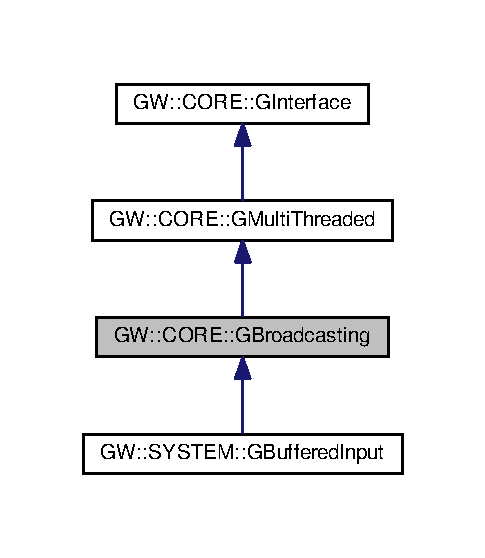
\includegraphics[width=233pt]{classGW_1_1CORE_1_1GBroadcasting__inherit__graph}
\end{center}
\end{figure}


Collaboration diagram for GW\+:\+:C\+O\+RE\+:\+:G\+Broadcasting\+:
\nopagebreak
\begin{figure}[H]
\begin{center}
\leavevmode
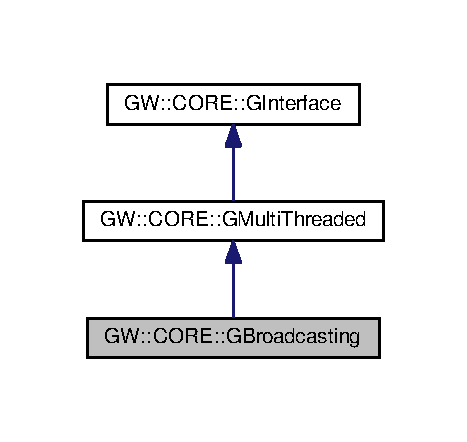
\includegraphics[width=224pt]{classGW_1_1CORE_1_1GBroadcasting__coll__graph}
\end{center}
\end{figure}
\subsection*{Public Member Functions}
\begin{DoxyCompactItemize}
\item 
virtual \hyperlink{namespaceGW_a67a839e3df7ea8a5c5686613a7a3de21}{G\+Return} \hyperlink{classGW_1_1CORE_1_1GBroadcasting_a293251421ba1169016f722df2f5b573b}{Register\+Listener} (\hyperlink{classGW_1_1CORE_1_1GListener}{G\+Listener} $\ast$\+\_\+add\+Listener, unsigned long long \+\_\+event\+Mask)=0
\begin{DoxyCompactList}\small\item\em Any listener added to this class must receive all events unless otherwise specified by the \+\_\+event\+Mask (optional). \end{DoxyCompactList}\item 
virtual \hyperlink{namespaceGW_a67a839e3df7ea8a5c5686613a7a3de21}{G\+Return} \hyperlink{classGW_1_1CORE_1_1GBroadcasting_afd6b1f41b646c668b1fcce2580681dd5}{Deregister\+Listener} (\hyperlink{classGW_1_1CORE_1_1GListener}{G\+Listener} $\ast$\+\_\+remove\+Listener)=0
\begin{DoxyCompactList}\small\item\em A successfully deregistered listener will no longer receive events and have its reference count decremented by one. \end{DoxyCompactList}\end{DoxyCompactItemize}


\subsection{Detailed Description}
The \hyperlink{classGW_1_1CORE_1_1GBroadcasting}{G\+Broadcasting} Interface is capable of registering \& deregistering \hyperlink{classGW_1_1CORE_1_1GListener}{G\+Listener} interfaces. 

The G\+Broadcaster will notify all registered listeners with the listeners On\+Event function. The events being registered for can be filtered with the \+\_\+event\+Mask (optional). 

\subsection{Member Function Documentation}
\index{G\+W\+::\+C\+O\+R\+E\+::\+G\+Broadcasting@{G\+W\+::\+C\+O\+R\+E\+::\+G\+Broadcasting}!Deregister\+Listener@{Deregister\+Listener}}
\index{Deregister\+Listener@{Deregister\+Listener}!G\+W\+::\+C\+O\+R\+E\+::\+G\+Broadcasting@{G\+W\+::\+C\+O\+R\+E\+::\+G\+Broadcasting}}
\subsubsection[{\texorpdfstring{Deregister\+Listener(\+G\+Listener $\ast$\+\_\+remove\+Listener)=0}{DeregisterListener(GListener *_removeListener)=0}}]{\setlength{\rightskip}{0pt plus 5cm}virtual {\bf G\+Return} G\+W\+::\+C\+O\+R\+E\+::\+G\+Broadcasting\+::\+Deregister\+Listener (
\begin{DoxyParamCaption}
\item[{{\bf G\+Listener} $\ast$}]{\+\_\+remove\+Listener}
\end{DoxyParamCaption}
)\hspace{0.3cm}{\ttfamily [pure virtual]}}\hypertarget{classGW_1_1CORE_1_1GBroadcasting_afd6b1f41b646c668b1fcce2580681dd5}{}\label{classGW_1_1CORE_1_1GBroadcasting_afd6b1f41b646c668b1fcce2580681dd5}


A successfully deregistered listener will no longer receive events and have its reference count decremented by one. 


\begin{DoxyParams}[1]{Parameters}
\mbox{\tt in}  & {\em \+\_\+remove\+Listener} & The listener to deregister from events.\\
\hline
\end{DoxyParams}

\begin{DoxyRetVals}{Return values}
{\em S\+U\+C\+C\+E\+SS} & The listener was successfully deregistered. \\
\hline
\end{DoxyRetVals}
\index{G\+W\+::\+C\+O\+R\+E\+::\+G\+Broadcasting@{G\+W\+::\+C\+O\+R\+E\+::\+G\+Broadcasting}!Register\+Listener@{Register\+Listener}}
\index{Register\+Listener@{Register\+Listener}!G\+W\+::\+C\+O\+R\+E\+::\+G\+Broadcasting@{G\+W\+::\+C\+O\+R\+E\+::\+G\+Broadcasting}}
\subsubsection[{\texorpdfstring{Register\+Listener(\+G\+Listener $\ast$\+\_\+add\+Listener, unsigned long long \+\_\+event\+Mask)=0}{RegisterListener(GListener *_addListener, unsigned long long _eventMask)=0}}]{\setlength{\rightskip}{0pt plus 5cm}virtual {\bf G\+Return} G\+W\+::\+C\+O\+R\+E\+::\+G\+Broadcasting\+::\+Register\+Listener (
\begin{DoxyParamCaption}
\item[{{\bf G\+Listener} $\ast$}]{\+\_\+add\+Listener, }
\item[{unsigned long long}]{\+\_\+event\+Mask}
\end{DoxyParamCaption}
)\hspace{0.3cm}{\ttfamily [pure virtual]}}\hypertarget{classGW_1_1CORE_1_1GBroadcasting_a293251421ba1169016f722df2f5b573b}{}\label{classGW_1_1CORE_1_1GBroadcasting_a293251421ba1169016f722df2f5b573b}


Any listener added to this class must receive all events unless otherwise specified by the \+\_\+event\+Mask (optional). 

Listeners registered to a broadcaster will have their reference counts increased by one until deregistered.


\begin{DoxyParams}[1]{Parameters}
\mbox{\tt in}  & {\em \+\_\+add\+Listener} & The listener object that is registering for messages. \\
\hline
\mbox{\tt in}  & {\em \+\_\+event\+Mask} & The events the listener is registering for. 0 will register for all events.\\
\hline
\end{DoxyParams}

\begin{DoxyRetVals}{Return values}
{\em S\+U\+C\+C\+E\+SS} & The listener was successfully registered. \\
\hline
{\em R\+E\+D\+U\+N\+D\+A\+N\+T\+\_\+\+O\+P\+E\+R\+A\+T\+I\+ON} & The listener has already been registered by a previous call. \\
\hline
\end{DoxyRetVals}


The documentation for this class was generated from the following file\+:\begin{DoxyCompactItemize}
\item 
Interface/\+G\+\_\+\+Core/G\+Broadcasting.\+h\end{DoxyCompactItemize}

\hypertarget{classGW_1_1SYSTEM_1_1GBufferedInput}{}\section{GW\+::S\+Y\+S\+T\+EM\+::G\+Buffered\+Input Class Reference}
\label{classGW_1_1SYSTEM_1_1GBufferedInput}\index{GW::SYSTEM::GBufferedInput@{GW::SYSTEM::GBufferedInput}}


A Multi-\/threaded buffered input library.  




{\ttfamily \#include $<$G\+Buffered\+Input.\+h$>$}



Inheritance diagram for GW\+::S\+Y\+S\+T\+EM\+::G\+Buffered\+Input\+:
% FIG 0


Collaboration diagram for GW\+::S\+Y\+S\+T\+EM\+::G\+Buffered\+Input\+:
% FIG 1
\subsection*{Additional Inherited Members}


\subsection{Detailed Description}
A Multi-\/threaded buffered input library. 

Register with a \mbox{\hyperlink{classGW_1_1SYSTEM_1_1GBufferedInput}{G\+Buffered\+Input}} to receive mouse and keyboard events. 

The documentation for this class was generated from the following file\+:\begin{DoxyCompactItemize}
\item 
Interface/\+G\+\_\+\+System/G\+Buffered\+Input.\+h\end{DoxyCompactItemize}

\hypertarget{structGW_1_1SYSTEM_1_1GBUFFEREDINPUT__EVENT__DATA}{}\section{GW\+:\+:S\+Y\+S\+T\+EM\+:\+:G\+B\+U\+F\+F\+E\+R\+E\+D\+I\+N\+P\+U\+T\+\_\+\+E\+V\+E\+N\+T\+\_\+\+D\+A\+TA Struct Reference}
\label{structGW_1_1SYSTEM_1_1GBUFFEREDINPUT__EVENT__DATA}\index{G\+W\+::\+S\+Y\+S\+T\+E\+M\+::\+G\+B\+U\+F\+F\+E\+R\+E\+D\+I\+N\+P\+U\+T\+\_\+\+E\+V\+E\+N\+T\+\_\+\+D\+A\+TA@{G\+W\+::\+S\+Y\+S\+T\+E\+M\+::\+G\+B\+U\+F\+F\+E\+R\+E\+D\+I\+N\+P\+U\+T\+\_\+\+E\+V\+E\+N\+T\+\_\+\+D\+A\+TA}}


Ensure identical binary padding for structures on all platforms.  




{\ttfamily \#include $<$G\+Buffered\+Input.\+h$>$}

\subsection*{Public Attributes}
\begin{DoxyCompactItemize}
\item 
int \hyperlink{structGW_1_1SYSTEM_1_1GBUFFEREDINPUT__EVENT__DATA_abe62d14dd92dc136e8ab4f53ee26d794}{data}
\item 
int \hyperlink{structGW_1_1SYSTEM_1_1GBUFFEREDINPUT__EVENT__DATA_a055e18b0d2aa3135ca8237bb06a0b4cb}{x}
\item 
int \hyperlink{structGW_1_1SYSTEM_1_1GBUFFEREDINPUT__EVENT__DATA_a68facd2e2754c908ecf8b8ef4ce34e08}{y}
\item 
int \hyperlink{structGW_1_1SYSTEM_1_1GBUFFEREDINPUT__EVENT__DATA_a8c87335f76992eddba30abe7312b5b43}{screenX}
\item 
int \hyperlink{structGW_1_1SYSTEM_1_1GBUFFEREDINPUT__EVENT__DATA_a066fa9b2dc654907d13590612238354d}{screenY}
\item 
unsigned int \hyperlink{structGW_1_1SYSTEM_1_1GBUFFEREDINPUT__EVENT__DATA_a7a818ba319e6693b89099938368a699e}{key\+Mask}
\end{DoxyCompactItemize}


\subsection{Detailed Description}
Ensure identical binary padding for structures on all platforms. 

\hyperlink{structGW_1_1SYSTEM_1_1GBUFFEREDINPUT__EVENT__DATA}{G\+B\+U\+F\+F\+E\+R\+E\+D\+I\+N\+P\+U\+T\+\_\+\+E\+V\+E\+N\+T\+\_\+\+D\+A\+TA} will hold any information you may need about an \hyperlink{classInput}{Input} Event. 

\subsection{Member Data Documentation}
\index{G\+W\+::\+S\+Y\+S\+T\+E\+M\+::\+G\+B\+U\+F\+F\+E\+R\+E\+D\+I\+N\+P\+U\+T\+\_\+\+E\+V\+E\+N\+T\+\_\+\+D\+A\+TA@{G\+W\+::\+S\+Y\+S\+T\+E\+M\+::\+G\+B\+U\+F\+F\+E\+R\+E\+D\+I\+N\+P\+U\+T\+\_\+\+E\+V\+E\+N\+T\+\_\+\+D\+A\+TA}!data@{data}}
\index{data@{data}!G\+W\+::\+S\+Y\+S\+T\+E\+M\+::\+G\+B\+U\+F\+F\+E\+R\+E\+D\+I\+N\+P\+U\+T\+\_\+\+E\+V\+E\+N\+T\+\_\+\+D\+A\+TA@{G\+W\+::\+S\+Y\+S\+T\+E\+M\+::\+G\+B\+U\+F\+F\+E\+R\+E\+D\+I\+N\+P\+U\+T\+\_\+\+E\+V\+E\+N\+T\+\_\+\+D\+A\+TA}}
\subsubsection[{\texorpdfstring{data}{data}}]{\setlength{\rightskip}{0pt plus 5cm}int G\+W\+::\+S\+Y\+S\+T\+E\+M\+::\+G\+B\+U\+F\+F\+E\+R\+E\+D\+I\+N\+P\+U\+T\+\_\+\+E\+V\+E\+N\+T\+\_\+\+D\+A\+T\+A\+::data}\hypertarget{structGW_1_1SYSTEM_1_1GBUFFEREDINPUT__EVENT__DATA_abe62d14dd92dc136e8ab4f53ee26d794}{}\label{structGW_1_1SYSTEM_1_1GBUFFEREDINPUT__EVENT__DATA_abe62d14dd92dc136e8ab4f53ee26d794}
Data storing the key/button information. \index{G\+W\+::\+S\+Y\+S\+T\+E\+M\+::\+G\+B\+U\+F\+F\+E\+R\+E\+D\+I\+N\+P\+U\+T\+\_\+\+E\+V\+E\+N\+T\+\_\+\+D\+A\+TA@{G\+W\+::\+S\+Y\+S\+T\+E\+M\+::\+G\+B\+U\+F\+F\+E\+R\+E\+D\+I\+N\+P\+U\+T\+\_\+\+E\+V\+E\+N\+T\+\_\+\+D\+A\+TA}!key\+Mask@{key\+Mask}}
\index{key\+Mask@{key\+Mask}!G\+W\+::\+S\+Y\+S\+T\+E\+M\+::\+G\+B\+U\+F\+F\+E\+R\+E\+D\+I\+N\+P\+U\+T\+\_\+\+E\+V\+E\+N\+T\+\_\+\+D\+A\+TA@{G\+W\+::\+S\+Y\+S\+T\+E\+M\+::\+G\+B\+U\+F\+F\+E\+R\+E\+D\+I\+N\+P\+U\+T\+\_\+\+E\+V\+E\+N\+T\+\_\+\+D\+A\+TA}}
\subsubsection[{\texorpdfstring{key\+Mask}{keyMask}}]{\setlength{\rightskip}{0pt plus 5cm}unsigned int G\+W\+::\+S\+Y\+S\+T\+E\+M\+::\+G\+B\+U\+F\+F\+E\+R\+E\+D\+I\+N\+P\+U\+T\+\_\+\+E\+V\+E\+N\+T\+\_\+\+D\+A\+T\+A\+::key\+Mask}\hypertarget{structGW_1_1SYSTEM_1_1GBUFFEREDINPUT__EVENT__DATA_a7a818ba319e6693b89099938368a699e}{}\label{structGW_1_1SYSTEM_1_1GBUFFEREDINPUT__EVENT__DATA_a7a818ba319e6693b89099938368a699e}
Bit flags for (Caps\+Lock, Num\+Lock, Scroll\+Lock, Shift, and Control). See \hyperlink{GKeyDefines_8h_source}{G\+Key\+Defines.\+h} for list of key\+Mask defines. \index{G\+W\+::\+S\+Y\+S\+T\+E\+M\+::\+G\+B\+U\+F\+F\+E\+R\+E\+D\+I\+N\+P\+U\+T\+\_\+\+E\+V\+E\+N\+T\+\_\+\+D\+A\+TA@{G\+W\+::\+S\+Y\+S\+T\+E\+M\+::\+G\+B\+U\+F\+F\+E\+R\+E\+D\+I\+N\+P\+U\+T\+\_\+\+E\+V\+E\+N\+T\+\_\+\+D\+A\+TA}!screenX@{screenX}}
\index{screenX@{screenX}!G\+W\+::\+S\+Y\+S\+T\+E\+M\+::\+G\+B\+U\+F\+F\+E\+R\+E\+D\+I\+N\+P\+U\+T\+\_\+\+E\+V\+E\+N\+T\+\_\+\+D\+A\+TA@{G\+W\+::\+S\+Y\+S\+T\+E\+M\+::\+G\+B\+U\+F\+F\+E\+R\+E\+D\+I\+N\+P\+U\+T\+\_\+\+E\+V\+E\+N\+T\+\_\+\+D\+A\+TA}}
\subsubsection[{\texorpdfstring{screenX}{screenX}}]{\setlength{\rightskip}{0pt plus 5cm}int G\+W\+::\+S\+Y\+S\+T\+E\+M\+::\+G\+B\+U\+F\+F\+E\+R\+E\+D\+I\+N\+P\+U\+T\+\_\+\+E\+V\+E\+N\+T\+\_\+\+D\+A\+T\+A\+::screenX}\hypertarget{structGW_1_1SYSTEM_1_1GBUFFEREDINPUT__EVENT__DATA_a8c87335f76992eddba30abe7312b5b43}{}\label{structGW_1_1SYSTEM_1_1GBUFFEREDINPUT__EVENT__DATA_a8c87335f76992eddba30abe7312b5b43}
Screen Mouse position x when event is sent. \index{G\+W\+::\+S\+Y\+S\+T\+E\+M\+::\+G\+B\+U\+F\+F\+E\+R\+E\+D\+I\+N\+P\+U\+T\+\_\+\+E\+V\+E\+N\+T\+\_\+\+D\+A\+TA@{G\+W\+::\+S\+Y\+S\+T\+E\+M\+::\+G\+B\+U\+F\+F\+E\+R\+E\+D\+I\+N\+P\+U\+T\+\_\+\+E\+V\+E\+N\+T\+\_\+\+D\+A\+TA}!screenY@{screenY}}
\index{screenY@{screenY}!G\+W\+::\+S\+Y\+S\+T\+E\+M\+::\+G\+B\+U\+F\+F\+E\+R\+E\+D\+I\+N\+P\+U\+T\+\_\+\+E\+V\+E\+N\+T\+\_\+\+D\+A\+TA@{G\+W\+::\+S\+Y\+S\+T\+E\+M\+::\+G\+B\+U\+F\+F\+E\+R\+E\+D\+I\+N\+P\+U\+T\+\_\+\+E\+V\+E\+N\+T\+\_\+\+D\+A\+TA}}
\subsubsection[{\texorpdfstring{screenY}{screenY}}]{\setlength{\rightskip}{0pt plus 5cm}int G\+W\+::\+S\+Y\+S\+T\+E\+M\+::\+G\+B\+U\+F\+F\+E\+R\+E\+D\+I\+N\+P\+U\+T\+\_\+\+E\+V\+E\+N\+T\+\_\+\+D\+A\+T\+A\+::screenY}\hypertarget{structGW_1_1SYSTEM_1_1GBUFFEREDINPUT__EVENT__DATA_a066fa9b2dc654907d13590612238354d}{}\label{structGW_1_1SYSTEM_1_1GBUFFEREDINPUT__EVENT__DATA_a066fa9b2dc654907d13590612238354d}
Screen Mouse position y when event is sent. \index{G\+W\+::\+S\+Y\+S\+T\+E\+M\+::\+G\+B\+U\+F\+F\+E\+R\+E\+D\+I\+N\+P\+U\+T\+\_\+\+E\+V\+E\+N\+T\+\_\+\+D\+A\+TA@{G\+W\+::\+S\+Y\+S\+T\+E\+M\+::\+G\+B\+U\+F\+F\+E\+R\+E\+D\+I\+N\+P\+U\+T\+\_\+\+E\+V\+E\+N\+T\+\_\+\+D\+A\+TA}!x@{x}}
\index{x@{x}!G\+W\+::\+S\+Y\+S\+T\+E\+M\+::\+G\+B\+U\+F\+F\+E\+R\+E\+D\+I\+N\+P\+U\+T\+\_\+\+E\+V\+E\+N\+T\+\_\+\+D\+A\+TA@{G\+W\+::\+S\+Y\+S\+T\+E\+M\+::\+G\+B\+U\+F\+F\+E\+R\+E\+D\+I\+N\+P\+U\+T\+\_\+\+E\+V\+E\+N\+T\+\_\+\+D\+A\+TA}}
\subsubsection[{\texorpdfstring{x}{x}}]{\setlength{\rightskip}{0pt plus 5cm}int G\+W\+::\+S\+Y\+S\+T\+E\+M\+::\+G\+B\+U\+F\+F\+E\+R\+E\+D\+I\+N\+P\+U\+T\+\_\+\+E\+V\+E\+N\+T\+\_\+\+D\+A\+T\+A\+::x}\hypertarget{structGW_1_1SYSTEM_1_1GBUFFEREDINPUT__EVENT__DATA_a055e18b0d2aa3135ca8237bb06a0b4cb}{}\label{structGW_1_1SYSTEM_1_1GBUFFEREDINPUT__EVENT__DATA_a055e18b0d2aa3135ca8237bb06a0b4cb}
Window Mouse position x when event is sent. \index{G\+W\+::\+S\+Y\+S\+T\+E\+M\+::\+G\+B\+U\+F\+F\+E\+R\+E\+D\+I\+N\+P\+U\+T\+\_\+\+E\+V\+E\+N\+T\+\_\+\+D\+A\+TA@{G\+W\+::\+S\+Y\+S\+T\+E\+M\+::\+G\+B\+U\+F\+F\+E\+R\+E\+D\+I\+N\+P\+U\+T\+\_\+\+E\+V\+E\+N\+T\+\_\+\+D\+A\+TA}!y@{y}}
\index{y@{y}!G\+W\+::\+S\+Y\+S\+T\+E\+M\+::\+G\+B\+U\+F\+F\+E\+R\+E\+D\+I\+N\+P\+U\+T\+\_\+\+E\+V\+E\+N\+T\+\_\+\+D\+A\+TA@{G\+W\+::\+S\+Y\+S\+T\+E\+M\+::\+G\+B\+U\+F\+F\+E\+R\+E\+D\+I\+N\+P\+U\+T\+\_\+\+E\+V\+E\+N\+T\+\_\+\+D\+A\+TA}}
\subsubsection[{\texorpdfstring{y}{y}}]{\setlength{\rightskip}{0pt plus 5cm}int G\+W\+::\+S\+Y\+S\+T\+E\+M\+::\+G\+B\+U\+F\+F\+E\+R\+E\+D\+I\+N\+P\+U\+T\+\_\+\+E\+V\+E\+N\+T\+\_\+\+D\+A\+T\+A\+::y}\hypertarget{structGW_1_1SYSTEM_1_1GBUFFEREDINPUT__EVENT__DATA_a68facd2e2754c908ecf8b8ef4ce34e08}{}\label{structGW_1_1SYSTEM_1_1GBUFFEREDINPUT__EVENT__DATA_a68facd2e2754c908ecf8b8ef4ce34e08}
Window Mouse position y when event is sent. 

The documentation for this struct was generated from the following file\+:\begin{DoxyCompactItemize}
\item 
Interface/\+G\+\_\+\+System/G\+Buffered\+Input.\+h\end{DoxyCompactItemize}

\hypertarget{classGW_1_1SYSTEM_1_1GFile}{}\section{GW\+:\+:S\+Y\+S\+T\+EM\+:\+:G\+File Class Reference}
\label{classGW_1_1SYSTEM_1_1GFile}\index{G\+W\+::\+S\+Y\+S\+T\+E\+M\+::\+G\+File@{G\+W\+::\+S\+Y\+S\+T\+E\+M\+::\+G\+File}}


Cross platform File\+I\+O/\+Directory handling.  




{\ttfamily \#include $<$G\+File.\+h$>$}



Inheritance diagram for GW\+:\+:S\+Y\+S\+T\+EM\+:\+:G\+File\+:
\nopagebreak
\begin{figure}[H]
\begin{center}
\leavevmode
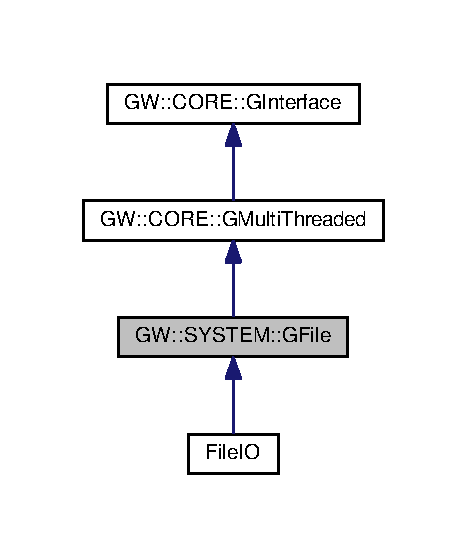
\includegraphics[width=224pt]{classGW_1_1SYSTEM_1_1GFile__inherit__graph}
\end{center}
\end{figure}


Collaboration diagram for GW\+:\+:S\+Y\+S\+T\+EM\+:\+:G\+File\+:
\nopagebreak
\begin{figure}[H]
\begin{center}
\leavevmode
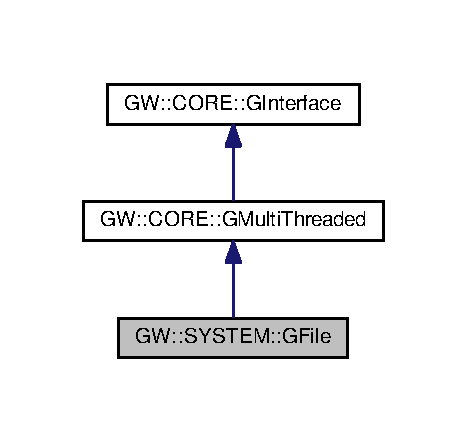
\includegraphics[width=224pt]{classGW_1_1SYSTEM_1_1GFile__coll__graph}
\end{center}
\end{figure}
\subsection*{Public Member Functions}
\begin{DoxyCompactItemize}
\item 
virtual \hyperlink{namespaceGW_a67a839e3df7ea8a5c5686613a7a3de21}{G\+Return} \hyperlink{classGW_1_1SYSTEM_1_1GFile_a2744359d5d258b1b59d139101c6809ce}{Open\+Binary\+Read} (const char $\ast$const \+\_\+file)=0
\begin{DoxyCompactList}\small\item\em Opens a file for binary read. \end{DoxyCompactList}\item 
virtual \hyperlink{namespaceGW_a67a839e3df7ea8a5c5686613a7a3de21}{G\+Return} \hyperlink{classGW_1_1SYSTEM_1_1GFile_a8d5f335bbc6f7c6d798ed27718aa2347}{Open\+Binary\+Write} (const char $\ast$const \+\_\+file)=0
\begin{DoxyCompactList}\small\item\em Opens a file for binary write with truncation. \end{DoxyCompactList}\item 
virtual \hyperlink{namespaceGW_a67a839e3df7ea8a5c5686613a7a3de21}{G\+Return} \hyperlink{classGW_1_1SYSTEM_1_1GFile_a63311236692181f99fd393fe8e1ca9fc}{Append\+Binary\+Write} (const char $\ast$const \+\_\+file)=0
\begin{DoxyCompactList}\small\item\em Opens a file for binary write with append. \end{DoxyCompactList}\item 
virtual \hyperlink{namespaceGW_a67a839e3df7ea8a5c5686613a7a3de21}{G\+Return} \hyperlink{classGW_1_1SYSTEM_1_1GFile_ac3ece72ce30e4d1a1c426c53a7a8354a}{Open\+Text\+Read} (const char $\ast$const \+\_\+file)=0
\begin{DoxyCompactList}\small\item\em Opens a file for text read. \end{DoxyCompactList}\item 
virtual \hyperlink{namespaceGW_a67a839e3df7ea8a5c5686613a7a3de21}{G\+Return} \hyperlink{classGW_1_1SYSTEM_1_1GFile_aebd3e32736b994c0296b7575ab0a2759}{Open\+Text\+Write} (const char $\ast$const \+\_\+file)=0
\begin{DoxyCompactList}\small\item\em Opens a file for text write with truncation. \end{DoxyCompactList}\item 
virtual \hyperlink{namespaceGW_a67a839e3df7ea8a5c5686613a7a3de21}{G\+Return} \hyperlink{classGW_1_1SYSTEM_1_1GFile_a72e40b3234a2384738d8db6e958f4782}{Append\+Text\+Write} (const char $\ast$const \+\_\+file)=0
\begin{DoxyCompactList}\small\item\em Opens a file for text write with append. \end{DoxyCompactList}\item 
virtual \hyperlink{namespaceGW_a67a839e3df7ea8a5c5686613a7a3de21}{G\+Return} \hyperlink{classGW_1_1SYSTEM_1_1GFile_ae9906414c159e9f1156b5ff6ad511c31}{Write} (const char $\ast$const \+\_\+in\+Data, unsigned int \+\_\+num\+Bytes)=0
\begin{DoxyCompactList}\small\item\em Writes binary data to the currently opened file. \end{DoxyCompactList}\item 
virtual \hyperlink{namespaceGW_a67a839e3df7ea8a5c5686613a7a3de21}{G\+Return} \hyperlink{classGW_1_1SYSTEM_1_1GFile_a1aaa026cba3d37abaaa2b408cd5d322d}{Read} (char $\ast$\+\_\+out\+Data, unsigned int \+\_\+num\+Bytes)=0
\begin{DoxyCompactList}\small\item\em Reads binary from the currently opened file. \end{DoxyCompactList}\item 
virtual \hyperlink{namespaceGW_a67a839e3df7ea8a5c5686613a7a3de21}{G\+Return} \hyperlink{classGW_1_1SYSTEM_1_1GFile_a7c57570575c63ae98f71232660d1b911}{Write\+Line} (const char $\ast$const \+\_\+in\+Data)=0
\begin{DoxyCompactList}\small\item\em Writes text to the currently opened file. \end{DoxyCompactList}\item 
virtual \hyperlink{namespaceGW_a67a839e3df7ea8a5c5686613a7a3de21}{G\+Return} \hyperlink{classGW_1_1SYSTEM_1_1GFile_ae9e072091ffe55f2f7697cb1d3eaec79}{Read\+Line} (char $\ast$\+\_\+out\+Data, unsigned int \+\_\+out\+Data\+Size, char \+\_\+delimiter)=0
\begin{DoxyCompactList}\small\item\em Reads text to the currently opened file. \end{DoxyCompactList}\item 
virtual \hyperlink{namespaceGW_a67a839e3df7ea8a5c5686613a7a3de21}{G\+Return} \hyperlink{classGW_1_1SYSTEM_1_1GFile_ae661d107c461145bb095dcfc76519f54}{Close\+File} ()=0
\begin{DoxyCompactList}\small\item\em Flushes and closes the current file. \end{DoxyCompactList}\item 
virtual \hyperlink{namespaceGW_a67a839e3df7ea8a5c5686613a7a3de21}{G\+Return} \hyperlink{classGW_1_1SYSTEM_1_1GFile_ae3105b637ef87af268722a696b8657a9}{Flush\+File} ()=0
\begin{DoxyCompactList}\small\item\em Flushes the current file. \end{DoxyCompactList}\item 
virtual \hyperlink{namespaceGW_a67a839e3df7ea8a5c5686613a7a3de21}{G\+Return} \hyperlink{classGW_1_1SYSTEM_1_1GFile_ab28d2e7ecf3ac893df88603e5448561a}{Set\+Current\+Working\+Directory} (const char $\ast$const \+\_\+dir)=0
\begin{DoxyCompactList}\small\item\em Changes the current working directory. \end{DoxyCompactList}\item 
virtual \hyperlink{namespaceGW_a67a839e3df7ea8a5c5686613a7a3de21}{G\+Return} \hyperlink{classGW_1_1SYSTEM_1_1GFile_a6853b717e838d1b3a54f22449a37d764}{Get\+Current\+Working\+Directory} (char $\ast$\+\_\+out\+Dir, unsigned int \+\_\+dir\+Size)=0
\begin{DoxyCompactList}\small\item\em Retrieves the absolute path of the current working directory. \end{DoxyCompactList}\item 
virtual \hyperlink{namespaceGW_a67a839e3df7ea8a5c5686613a7a3de21}{G\+Return} \hyperlink{classGW_1_1SYSTEM_1_1GFile_ac2de86bf6cf61455577efc47277ecb94}{Get\+Directory\+Size} (unsigned int \&\+\_\+out\+Size)=0
\begin{DoxyCompactList}\small\item\em Gets the number of files in the current working directory. \end{DoxyCompactList}\item 
virtual \hyperlink{namespaceGW_a67a839e3df7ea8a5c5686613a7a3de21}{G\+Return} \hyperlink{classGW_1_1SYSTEM_1_1GFile_ae062d19f84d120adea94756d1d26e41e}{Get\+Files\+From\+Directory} (char $\ast$\+\_\+out\+Files\mbox{[}$\,$\mbox{]}, unsigned int \+\_\+num\+Files, unsigned int \+\_\+file\+Name\+Size)=0
\begin{DoxyCompactList}\small\item\em Gets the names of all files in the current working directory. \end{DoxyCompactList}\item 
virtual \hyperlink{namespaceGW_a67a839e3df7ea8a5c5686613a7a3de21}{G\+Return} \hyperlink{classGW_1_1SYSTEM_1_1GFile_a2f4cba2dad96fa4c894545f43fee64b5}{Get\+File\+Size} (const char $\ast$const \+\_\+file, unsigned int \&\+\_\+out\+Size)=0
\begin{DoxyCompactList}\small\item\em Gets the size of the specified file in bytes. \end{DoxyCompactList}\end{DoxyCompactItemize}


\subsection{Detailed Description}
Cross platform File\+I\+O/\+Directory handling. 

Handles file input/output operations, as well as directory information and file information. Inherits from G\+Multi\+Threaded, therfore its implementation must be thread safe. 

\subsection{Member Function Documentation}
\index{G\+W\+::\+S\+Y\+S\+T\+E\+M\+::\+G\+File@{G\+W\+::\+S\+Y\+S\+T\+E\+M\+::\+G\+File}!Append\+Binary\+Write@{Append\+Binary\+Write}}
\index{Append\+Binary\+Write@{Append\+Binary\+Write}!G\+W\+::\+S\+Y\+S\+T\+E\+M\+::\+G\+File@{G\+W\+::\+S\+Y\+S\+T\+E\+M\+::\+G\+File}}
\subsubsection[{\texorpdfstring{Append\+Binary\+Write(const char $\ast$const \+\_\+file)=0}{AppendBinaryWrite(const char *const _file)=0}}]{\setlength{\rightskip}{0pt plus 5cm}virtual {\bf G\+Return} G\+W\+::\+S\+Y\+S\+T\+E\+M\+::\+G\+File\+::\+Append\+Binary\+Write (
\begin{DoxyParamCaption}
\item[{const char $\ast$const}]{\+\_\+file}
\end{DoxyParamCaption}
)\hspace{0.3cm}{\ttfamily [pure virtual]}}\hypertarget{classGW_1_1SYSTEM_1_1GFile_a63311236692181f99fd393fe8e1ca9fc}{}\label{classGW_1_1SYSTEM_1_1GFile_a63311236692181f99fd393fe8e1ca9fc}


Opens a file for binary write with append. 

The file name passed into the function should be passed like it is a relative path. The function will look in the current working directory for the file. If the file is not found in the current working directory, the file will be created in the current working directory. File can now be written to with \hyperlink{classGW_1_1SYSTEM_1_1GFile_ae9906414c159e9f1156b5ff6ad511c31}{Write()}.


\begin{DoxyParams}[1]{Parameters}
\mbox{\tt in}  & {\em \+\_\+file} & The file name of the file to open.\\
\hline
\end{DoxyParams}

\begin{DoxyRetVals}{Return values}
{\em S\+U\+C\+C\+E\+SS} & Succesfully opened the file. \\
\hline
{\em F\+A\+I\+L\+U\+RE} & A file is already open or the file could not be found/created. \\
\hline
{\em I\+N\+V\+A\+L\+I\+D\+\_\+\+A\+R\+G\+U\+M\+E\+NT} & A nullptr was passed in. \\
\hline
\end{DoxyRetVals}


Implemented in \hyperlink{classFileIO_ab26fc846b30446edf28ac922759c9e5e}{File\+IO}.

\index{G\+W\+::\+S\+Y\+S\+T\+E\+M\+::\+G\+File@{G\+W\+::\+S\+Y\+S\+T\+E\+M\+::\+G\+File}!Append\+Text\+Write@{Append\+Text\+Write}}
\index{Append\+Text\+Write@{Append\+Text\+Write}!G\+W\+::\+S\+Y\+S\+T\+E\+M\+::\+G\+File@{G\+W\+::\+S\+Y\+S\+T\+E\+M\+::\+G\+File}}
\subsubsection[{\texorpdfstring{Append\+Text\+Write(const char $\ast$const \+\_\+file)=0}{AppendTextWrite(const char *const _file)=0}}]{\setlength{\rightskip}{0pt plus 5cm}virtual {\bf G\+Return} G\+W\+::\+S\+Y\+S\+T\+E\+M\+::\+G\+File\+::\+Append\+Text\+Write (
\begin{DoxyParamCaption}
\item[{const char $\ast$const}]{\+\_\+file}
\end{DoxyParamCaption}
)\hspace{0.3cm}{\ttfamily [pure virtual]}}\hypertarget{classGW_1_1SYSTEM_1_1GFile_a72e40b3234a2384738d8db6e958f4782}{}\label{classGW_1_1SYSTEM_1_1GFile_a72e40b3234a2384738d8db6e958f4782}


Opens a file for text write with append. 

The file name passed into the function should be passed like it is a relative path. The function will look in the current working directory for the file. If the file is not found in the current working directory, the file will be created in the current working directory. File can now be written to with \hyperlink{classGW_1_1SYSTEM_1_1GFile_ae9906414c159e9f1156b5ff6ad511c31}{Write()}.


\begin{DoxyParams}[1]{Parameters}
\mbox{\tt in}  & {\em \+\_\+file} & The file name of the file to open.\\
\hline
\end{DoxyParams}

\begin{DoxyRetVals}{Return values}
{\em S\+U\+C\+C\+E\+SS} & Succesfully opened the file. \\
\hline
{\em F\+A\+I\+L\+U\+RE} & A file is already open or the file could not be found/created. \\
\hline
{\em I\+N\+V\+A\+L\+I\+D\+\_\+\+A\+R\+G\+U\+M\+E\+NT} & A nullptr was passed in. \\
\hline
\end{DoxyRetVals}


Implemented in \hyperlink{classFileIO_afd4e0d14b85d8c0aded66bd946c291f4}{File\+IO}.

\index{G\+W\+::\+S\+Y\+S\+T\+E\+M\+::\+G\+File@{G\+W\+::\+S\+Y\+S\+T\+E\+M\+::\+G\+File}!Close\+File@{Close\+File}}
\index{Close\+File@{Close\+File}!G\+W\+::\+S\+Y\+S\+T\+E\+M\+::\+G\+File@{G\+W\+::\+S\+Y\+S\+T\+E\+M\+::\+G\+File}}
\subsubsection[{\texorpdfstring{Close\+File()=0}{CloseFile()=0}}]{\setlength{\rightskip}{0pt plus 5cm}virtual {\bf G\+Return} G\+W\+::\+S\+Y\+S\+T\+E\+M\+::\+G\+File\+::\+Close\+File (
\begin{DoxyParamCaption}
{}
\end{DoxyParamCaption}
)\hspace{0.3cm}{\ttfamily [pure virtual]}}\hypertarget{classGW_1_1SYSTEM_1_1GFile_ae661d107c461145bb095dcfc76519f54}{}\label{classGW_1_1SYSTEM_1_1GFile_ae661d107c461145bb095dcfc76519f54}


Flushes and closes the current file. 


\begin{DoxyRetVals}{Return values}
{\em S\+U\+C\+C\+E\+SS} & File successfully flushed and closed. \\
\hline
{\em F\+A\+I\+L\+U\+RE} & A file is not currently open. \\
\hline
\end{DoxyRetVals}


Implemented in \hyperlink{classFileIO_a906610c8653ba8ca476dc46679851590}{File\+IO}.

\index{G\+W\+::\+S\+Y\+S\+T\+E\+M\+::\+G\+File@{G\+W\+::\+S\+Y\+S\+T\+E\+M\+::\+G\+File}!Flush\+File@{Flush\+File}}
\index{Flush\+File@{Flush\+File}!G\+W\+::\+S\+Y\+S\+T\+E\+M\+::\+G\+File@{G\+W\+::\+S\+Y\+S\+T\+E\+M\+::\+G\+File}}
\subsubsection[{\texorpdfstring{Flush\+File()=0}{FlushFile()=0}}]{\setlength{\rightskip}{0pt plus 5cm}virtual {\bf G\+Return} G\+W\+::\+S\+Y\+S\+T\+E\+M\+::\+G\+File\+::\+Flush\+File (
\begin{DoxyParamCaption}
{}
\end{DoxyParamCaption}
)\hspace{0.3cm}{\ttfamily [pure virtual]}}\hypertarget{classGW_1_1SYSTEM_1_1GFile_ae3105b637ef87af268722a696b8657a9}{}\label{classGW_1_1SYSTEM_1_1GFile_ae3105b637ef87af268722a696b8657a9}


Flushes the current file. 


\begin{DoxyRetVals}{Return values}
{\em S\+U\+C\+C\+E\+SS} & File successfully flushed. \\
\hline
{\em F\+A\+I\+L\+U\+RE} & A file is not currently open. \\
\hline
\end{DoxyRetVals}


Implemented in \hyperlink{classFileIO_a8e5afdb1a734f37e422ff0147561a3a1}{File\+IO}.

\index{G\+W\+::\+S\+Y\+S\+T\+E\+M\+::\+G\+File@{G\+W\+::\+S\+Y\+S\+T\+E\+M\+::\+G\+File}!Get\+Current\+Working\+Directory@{Get\+Current\+Working\+Directory}}
\index{Get\+Current\+Working\+Directory@{Get\+Current\+Working\+Directory}!G\+W\+::\+S\+Y\+S\+T\+E\+M\+::\+G\+File@{G\+W\+::\+S\+Y\+S\+T\+E\+M\+::\+G\+File}}
\subsubsection[{\texorpdfstring{Get\+Current\+Working\+Directory(char $\ast$\+\_\+out\+Dir, unsigned int \+\_\+dir\+Size)=0}{GetCurrentWorkingDirectory(char *_outDir, unsigned int _dirSize)=0}}]{\setlength{\rightskip}{0pt plus 5cm}virtual {\bf G\+Return} G\+W\+::\+S\+Y\+S\+T\+E\+M\+::\+G\+File\+::\+Get\+Current\+Working\+Directory (
\begin{DoxyParamCaption}
\item[{char $\ast$}]{\+\_\+out\+Dir, }
\item[{unsigned int}]{\+\_\+dir\+Size}
\end{DoxyParamCaption}
)\hspace{0.3cm}{\ttfamily [pure virtual]}}\hypertarget{classGW_1_1SYSTEM_1_1GFile_a6853b717e838d1b3a54f22449a37d764}{}\label{classGW_1_1SYSTEM_1_1GFile_a6853b717e838d1b3a54f22449a37d764}


Retrieves the absolute path of the current working directory. 

This is the directory we will look into for any file Open commands. This is by Windows standard guaranteed to be 255 or less.


\begin{DoxyParams}[1]{Parameters}
\mbox{\tt out}  & {\em \+\_\+out\+Dir} & An absolute path to the directory to set as the current working directory. \\
\hline
\mbox{\tt in}  & {\em \+\_\+dir\+Size} & The size of \+\_\+out\+Dir.\\
\hline
\end{DoxyParams}

\begin{DoxyRetVals}{Return values}
{\em S\+U\+C\+C\+E\+SS} & Successfully obtained the working directory. \\
\hline
{\em F\+A\+I\+L\+U\+RE} & The current working directory is invalid or \+\_\+out\+Dir was not big enough. \+\_\+out\+Dir will be null. \\
\hline
{\em I\+N\+V\+A\+L\+I\+D\+\_\+\+A\+R\+G\+U\+M\+E\+NT} & A nullptr was passed in or the size is 0. \\
\hline
\end{DoxyRetVals}


Implemented in \hyperlink{classFileIO_a41a1859ffe3ebd76005f264af0b1ea66}{File\+IO}.

\index{G\+W\+::\+S\+Y\+S\+T\+E\+M\+::\+G\+File@{G\+W\+::\+S\+Y\+S\+T\+E\+M\+::\+G\+File}!Get\+Directory\+Size@{Get\+Directory\+Size}}
\index{Get\+Directory\+Size@{Get\+Directory\+Size}!G\+W\+::\+S\+Y\+S\+T\+E\+M\+::\+G\+File@{G\+W\+::\+S\+Y\+S\+T\+E\+M\+::\+G\+File}}
\subsubsection[{\texorpdfstring{Get\+Directory\+Size(unsigned int \&\+\_\+out\+Size)=0}{GetDirectorySize(unsigned int &_outSize)=0}}]{\setlength{\rightskip}{0pt plus 5cm}virtual {\bf G\+Return} G\+W\+::\+S\+Y\+S\+T\+E\+M\+::\+G\+File\+::\+Get\+Directory\+Size (
\begin{DoxyParamCaption}
\item[{unsigned int \&}]{\+\_\+out\+Size}
\end{DoxyParamCaption}
)\hspace{0.3cm}{\ttfamily [pure virtual]}}\hypertarget{classGW_1_1SYSTEM_1_1GFile_ac2de86bf6cf61455577efc47277ecb94}{}\label{classGW_1_1SYSTEM_1_1GFile_ac2de86bf6cf61455577efc47277ecb94}


Gets the number of files in the current working directory. 


\begin{DoxyParams}[1]{Parameters}
\mbox{\tt out}  & {\em \+\_\+out\+Size} & The number of files in the directory.\\
\hline
\end{DoxyParams}

\begin{DoxyRetVals}{Return values}
{\em S\+U\+C\+C\+E\+SS} & Successfully counted the files in the directory. \\
\hline
{\em F\+A\+I\+L\+U\+RE} & Either currently working directory is invalid or count failed. \+\_\+out\+Size will be -\/1. \\
\hline
\end{DoxyRetVals}


Implemented in \hyperlink{classFileIO_ae331f6c02948720d9cc5bcd2700d8cf7}{File\+IO}.

\index{G\+W\+::\+S\+Y\+S\+T\+E\+M\+::\+G\+File@{G\+W\+::\+S\+Y\+S\+T\+E\+M\+::\+G\+File}!Get\+Files\+From\+Directory@{Get\+Files\+From\+Directory}}
\index{Get\+Files\+From\+Directory@{Get\+Files\+From\+Directory}!G\+W\+::\+S\+Y\+S\+T\+E\+M\+::\+G\+File@{G\+W\+::\+S\+Y\+S\+T\+E\+M\+::\+G\+File}}
\subsubsection[{\texorpdfstring{Get\+Files\+From\+Directory(char $\ast$\+\_\+out\+Files[], unsigned int \+\_\+num\+Files, unsigned int \+\_\+file\+Name\+Size)=0}{GetFilesFromDirectory(char *_outFiles[], unsigned int _numFiles, unsigned int _fileNameSize)=0}}]{\setlength{\rightskip}{0pt plus 5cm}virtual {\bf G\+Return} G\+W\+::\+S\+Y\+S\+T\+E\+M\+::\+G\+File\+::\+Get\+Files\+From\+Directory (
\begin{DoxyParamCaption}
\item[{char $\ast$}]{\+\_\+out\+Files\mbox{[}$\,$\mbox{]}, }
\item[{unsigned int}]{\+\_\+num\+Files, }
\item[{unsigned int}]{\+\_\+file\+Name\+Size}
\end{DoxyParamCaption}
)\hspace{0.3cm}{\ttfamily [pure virtual]}}\hypertarget{classGW_1_1SYSTEM_1_1GFile_ae062d19f84d120adea94756d1d26e41e}{}\label{classGW_1_1SYSTEM_1_1GFile_ae062d19f84d120adea94756d1d26e41e}


Gets the names of all files in the current working directory. 

This function will retrieve just the file names and extensions. Any Open function using these names will assume the files are in the current working directory. Any change of the current working directory will make these names invalid until called again.


\begin{DoxyParams}[1]{Parameters}
\mbox{\tt out}  & {\em \+\_\+out\+Files} & Stores the names of the files retrieved. \\
\hline
\mbox{\tt in}  & {\em \+\_\+num\+Files} & The number of files. \\
\hline
\mbox{\tt in}  & {\em \+\_\+file\+Name\+Size} & The size of the file names.\\
\hline
\end{DoxyParams}

\begin{DoxyRetVals}{Return values}
{\em S\+U\+C\+C\+E\+SS} & Successfully retrieved the file names. \\
\hline
{\em F\+A\+I\+L\+U\+RE} & Either current working directory is invalid or obtaining file names failed. \\
\hline
\end{DoxyRetVals}


Implemented in \hyperlink{classFileIO_afd1b77afed3d853aaa01f14ecbc6b0e0}{File\+IO}.

\index{G\+W\+::\+S\+Y\+S\+T\+E\+M\+::\+G\+File@{G\+W\+::\+S\+Y\+S\+T\+E\+M\+::\+G\+File}!Get\+File\+Size@{Get\+File\+Size}}
\index{Get\+File\+Size@{Get\+File\+Size}!G\+W\+::\+S\+Y\+S\+T\+E\+M\+::\+G\+File@{G\+W\+::\+S\+Y\+S\+T\+E\+M\+::\+G\+File}}
\subsubsection[{\texorpdfstring{Get\+File\+Size(const char $\ast$const \+\_\+file, unsigned int \&\+\_\+out\+Size)=0}{GetFileSize(const char *const _file, unsigned int &_outSize)=0}}]{\setlength{\rightskip}{0pt plus 5cm}virtual {\bf G\+Return} G\+W\+::\+S\+Y\+S\+T\+E\+M\+::\+G\+File\+::\+Get\+File\+Size (
\begin{DoxyParamCaption}
\item[{const char $\ast$const}]{\+\_\+file, }
\item[{unsigned int \&}]{\+\_\+out\+Size}
\end{DoxyParamCaption}
)\hspace{0.3cm}{\ttfamily [pure virtual]}}\hypertarget{classGW_1_1SYSTEM_1_1GFile_a2f4cba2dad96fa4c894545f43fee64b5}{}\label{classGW_1_1SYSTEM_1_1GFile_a2f4cba2dad96fa4c894545f43fee64b5}


Gets the size of the specified file in bytes. 

The filename passed into this function should be passed as a relative path. This function will assume the file passed in is in the current working directory and will look for it there.


\begin{DoxyParams}[1]{Parameters}
\mbox{\tt in}  & {\em \+\_\+file} & The file to get the size of. \\
\hline
\mbox{\tt out}  & {\em \+\_\+out\+Size} & will store the size of the file.\\
\hline
\end{DoxyParams}

\begin{DoxyRetVals}{Return values}
{\em S\+U\+C\+C\+E\+SS} & Successfully retrieved the file size. \\
\hline
{\em F\+I\+L\+E\+\_\+\+N\+O\+T\+\_\+\+F\+O\+U\+ND} & Could not locate the file. Check that the current working directory is valid. \\
\hline
\end{DoxyRetVals}


Implemented in \hyperlink{classFileIO_a91ee3ceabd5d6097eed85466c26d2adb}{File\+IO}.

\index{G\+W\+::\+S\+Y\+S\+T\+E\+M\+::\+G\+File@{G\+W\+::\+S\+Y\+S\+T\+E\+M\+::\+G\+File}!Open\+Binary\+Read@{Open\+Binary\+Read}}
\index{Open\+Binary\+Read@{Open\+Binary\+Read}!G\+W\+::\+S\+Y\+S\+T\+E\+M\+::\+G\+File@{G\+W\+::\+S\+Y\+S\+T\+E\+M\+::\+G\+File}}
\subsubsection[{\texorpdfstring{Open\+Binary\+Read(const char $\ast$const \+\_\+file)=0}{OpenBinaryRead(const char *const _file)=0}}]{\setlength{\rightskip}{0pt plus 5cm}virtual {\bf G\+Return} G\+W\+::\+S\+Y\+S\+T\+E\+M\+::\+G\+File\+::\+Open\+Binary\+Read (
\begin{DoxyParamCaption}
\item[{const char $\ast$const}]{\+\_\+file}
\end{DoxyParamCaption}
)\hspace{0.3cm}{\ttfamily [pure virtual]}}\hypertarget{classGW_1_1SYSTEM_1_1GFile_a2744359d5d258b1b59d139101c6809ce}{}\label{classGW_1_1SYSTEM_1_1GFile_a2744359d5d258b1b59d139101c6809ce}


Opens a file for binary read. 

The file name passed into the function should be passed like it is a relative path. The function will look in the current working directory for the file. If the file is not found in the current working directory, the function will fail.


\begin{DoxyParams}[1]{Parameters}
\mbox{\tt in}  & {\em \+\_\+file} & The file name of the file to open.\\
\hline
\end{DoxyParams}

\begin{DoxyRetVals}{Return values}
{\em S\+U\+C\+C\+E\+SS} & Succesfully opened the file. \\
\hline
{\em F\+I\+L\+E\+\_\+\+N\+O\+T\+\_\+\+F\+O\+U\+ND} & File could not be found. \\
\hline
{\em F\+A\+I\+L\+U\+RE} & A file is already opened. \\
\hline
{\em I\+N\+V\+A\+L\+I\+D\+\_\+\+A\+R\+G\+U\+M\+E\+NT} & A null pointer was passed in. \\
\hline
\end{DoxyRetVals}


Implemented in \hyperlink{classFileIO_a0adeb88dd23bb5897e8315ab0029c835}{File\+IO}.

\index{G\+W\+::\+S\+Y\+S\+T\+E\+M\+::\+G\+File@{G\+W\+::\+S\+Y\+S\+T\+E\+M\+::\+G\+File}!Open\+Binary\+Write@{Open\+Binary\+Write}}
\index{Open\+Binary\+Write@{Open\+Binary\+Write}!G\+W\+::\+S\+Y\+S\+T\+E\+M\+::\+G\+File@{G\+W\+::\+S\+Y\+S\+T\+E\+M\+::\+G\+File}}
\subsubsection[{\texorpdfstring{Open\+Binary\+Write(const char $\ast$const \+\_\+file)=0}{OpenBinaryWrite(const char *const _file)=0}}]{\setlength{\rightskip}{0pt plus 5cm}virtual {\bf G\+Return} G\+W\+::\+S\+Y\+S\+T\+E\+M\+::\+G\+File\+::\+Open\+Binary\+Write (
\begin{DoxyParamCaption}
\item[{const char $\ast$const}]{\+\_\+file}
\end{DoxyParamCaption}
)\hspace{0.3cm}{\ttfamily [pure virtual]}}\hypertarget{classGW_1_1SYSTEM_1_1GFile_a8d5f335bbc6f7c6d798ed27718aa2347}{}\label{classGW_1_1SYSTEM_1_1GFile_a8d5f335bbc6f7c6d798ed27718aa2347}


Opens a file for binary write with truncation. 

The file name passed into the function should be passed like it is a relative path. The function will look in the current working directory for the file. If the file is not found in the current working directory, the file will be created in the current working directory. File can now be read from with \hyperlink{classGW_1_1SYSTEM_1_1GFile_a1aaa026cba3d37abaaa2b408cd5d322d}{Read()}.


\begin{DoxyParams}[1]{Parameters}
\mbox{\tt in}  & {\em \+\_\+file} & The file name of the file to open.\\
\hline
\end{DoxyParams}

\begin{DoxyRetVals}{Return values}
{\em S\+U\+C\+C\+E\+SS} & Succesfully opened the file. \\
\hline
{\em F\+A\+I\+L\+U\+RE} & A file is already open or file could not be found/created. \\
\hline
{\em I\+N\+V\+A\+L\+I\+D\+\_\+\+A\+R\+G\+U\+M\+E\+NT} & A nullptr was passed in. \\
\hline
\end{DoxyRetVals}


Implemented in \hyperlink{classFileIO_a5cd87c21a72ae2dba21a9f3e50841e6e}{File\+IO}.

\index{G\+W\+::\+S\+Y\+S\+T\+E\+M\+::\+G\+File@{G\+W\+::\+S\+Y\+S\+T\+E\+M\+::\+G\+File}!Open\+Text\+Read@{Open\+Text\+Read}}
\index{Open\+Text\+Read@{Open\+Text\+Read}!G\+W\+::\+S\+Y\+S\+T\+E\+M\+::\+G\+File@{G\+W\+::\+S\+Y\+S\+T\+E\+M\+::\+G\+File}}
\subsubsection[{\texorpdfstring{Open\+Text\+Read(const char $\ast$const \+\_\+file)=0}{OpenTextRead(const char *const _file)=0}}]{\setlength{\rightskip}{0pt plus 5cm}virtual {\bf G\+Return} G\+W\+::\+S\+Y\+S\+T\+E\+M\+::\+G\+File\+::\+Open\+Text\+Read (
\begin{DoxyParamCaption}
\item[{const char $\ast$const}]{\+\_\+file}
\end{DoxyParamCaption}
)\hspace{0.3cm}{\ttfamily [pure virtual]}}\hypertarget{classGW_1_1SYSTEM_1_1GFile_ac3ece72ce30e4d1a1c426c53a7a8354a}{}\label{classGW_1_1SYSTEM_1_1GFile_ac3ece72ce30e4d1a1c426c53a7a8354a}


Opens a file for text read. 

The file name passed into the function should be passed like it is a relative path. The function will look in the current working directory for the file. If the file is not found in the current working directory, the function will fail. File can now be written to with \hyperlink{classGW_1_1SYSTEM_1_1GFile_ae9906414c159e9f1156b5ff6ad511c31}{Write()}.


\begin{DoxyParams}[1]{Parameters}
\mbox{\tt in}  & {\em \+\_\+file} & The file name of the file to open.\\
\hline
\end{DoxyParams}

\begin{DoxyRetVals}{Return values}
{\em S\+U\+C\+C\+E\+SS} & Succesfully opened the file. \\
\hline
{\em F\+I\+L\+E\+\_\+\+N\+O\+T\+\_\+\+F\+O\+U\+ND} & File could not be found. \\
\hline
{\em F\+A\+I\+L\+U\+RE} & A file is already open. \\
\hline
{\em I\+N\+V\+A\+L\+I\+D\+\_\+\+A\+R\+G\+U\+M\+E\+NT} & A nullptr was passed in. \\
\hline
\end{DoxyRetVals}


Implemented in \hyperlink{classFileIO_a3d93902abce1baec299cd63891798681}{File\+IO}.

\index{G\+W\+::\+S\+Y\+S\+T\+E\+M\+::\+G\+File@{G\+W\+::\+S\+Y\+S\+T\+E\+M\+::\+G\+File}!Open\+Text\+Write@{Open\+Text\+Write}}
\index{Open\+Text\+Write@{Open\+Text\+Write}!G\+W\+::\+S\+Y\+S\+T\+E\+M\+::\+G\+File@{G\+W\+::\+S\+Y\+S\+T\+E\+M\+::\+G\+File}}
\subsubsection[{\texorpdfstring{Open\+Text\+Write(const char $\ast$const \+\_\+file)=0}{OpenTextWrite(const char *const _file)=0}}]{\setlength{\rightskip}{0pt plus 5cm}virtual {\bf G\+Return} G\+W\+::\+S\+Y\+S\+T\+E\+M\+::\+G\+File\+::\+Open\+Text\+Write (
\begin{DoxyParamCaption}
\item[{const char $\ast$const}]{\+\_\+file}
\end{DoxyParamCaption}
)\hspace{0.3cm}{\ttfamily [pure virtual]}}\hypertarget{classGW_1_1SYSTEM_1_1GFile_aebd3e32736b994c0296b7575ab0a2759}{}\label{classGW_1_1SYSTEM_1_1GFile_aebd3e32736b994c0296b7575ab0a2759}


Opens a file for text write with truncation. 

The file name passed into the function should be passed like it is a relative path. The function will look in the current working directory for the file. If the file is not found in the current working directory, the file will be created in the current working directory. File can now be read from with \hyperlink{classGW_1_1SYSTEM_1_1GFile_a1aaa026cba3d37abaaa2b408cd5d322d}{Read()}.


\begin{DoxyParams}[1]{Parameters}
\mbox{\tt in}  & {\em \+\_\+file} & The file name of the file to open.\\
\hline
\end{DoxyParams}

\begin{DoxyRetVals}{Return values}
{\em S\+U\+C\+C\+E\+SS} & Succesfully opened the file. \\
\hline
{\em F\+A\+I\+L\+U\+RE} & A file is already open or the file could not be found/created. \\
\hline
{\em I\+N\+V\+A\+L\+I\+D\+\_\+\+A\+R\+G\+U\+M\+E\+NT} & A nullptr was passed in. \\
\hline
\end{DoxyRetVals}


Implemented in \hyperlink{classFileIO_a4e51443206e9cf97dcac28719dbeb23e}{File\+IO}.

\index{G\+W\+::\+S\+Y\+S\+T\+E\+M\+::\+G\+File@{G\+W\+::\+S\+Y\+S\+T\+E\+M\+::\+G\+File}!Read@{Read}}
\index{Read@{Read}!G\+W\+::\+S\+Y\+S\+T\+E\+M\+::\+G\+File@{G\+W\+::\+S\+Y\+S\+T\+E\+M\+::\+G\+File}}
\subsubsection[{\texorpdfstring{Read(char $\ast$\+\_\+out\+Data, unsigned int \+\_\+num\+Bytes)=0}{Read(char *_outData, unsigned int _numBytes)=0}}]{\setlength{\rightskip}{0pt plus 5cm}virtual {\bf G\+Return} G\+W\+::\+S\+Y\+S\+T\+E\+M\+::\+G\+File\+::\+Read (
\begin{DoxyParamCaption}
\item[{char $\ast$}]{\+\_\+out\+Data, }
\item[{unsigned int}]{\+\_\+num\+Bytes}
\end{DoxyParamCaption}
)\hspace{0.3cm}{\ttfamily [pure virtual]}}\hypertarget{classGW_1_1SYSTEM_1_1GFile_a1aaa026cba3d37abaaa2b408cd5d322d}{}\label{classGW_1_1SYSTEM_1_1GFile_a1aaa026cba3d37abaaa2b408cd5d322d}


Reads binary from the currently opened file. 

Reads binary data and stores it into a char$\ast$ until the byte limit is reached.


\begin{DoxyParams}[1]{Parameters}
\mbox{\tt out}  & {\em \+\_\+out\+Data} & The variable to store the read in bytes. \\
\hline
\mbox{\tt in}  & {\em \+\_\+num\+Bytes} & The number of bytes to read in from the file.\\
\hline
\end{DoxyParams}

\begin{DoxyRetVals}{Return values}
{\em S\+U\+C\+C\+E\+SS} & Successful read. \\
\hline
{\em F\+A\+I\+L\+U\+RE} & Either file is not open or read failed. \+\_\+out\+Data will be null. \\
\hline
{\em I\+N\+V\+A\+L\+I\+D\+\_\+\+A\+R\+G\+U\+M\+E\+NT} & A byte size of 0 was passed in. \\
\hline
\end{DoxyRetVals}


Implemented in \hyperlink{classFileIO_adb5270ace70c0189525a7c21c5be31b9}{File\+IO}.

\index{G\+W\+::\+S\+Y\+S\+T\+E\+M\+::\+G\+File@{G\+W\+::\+S\+Y\+S\+T\+E\+M\+::\+G\+File}!Read\+Line@{Read\+Line}}
\index{Read\+Line@{Read\+Line}!G\+W\+::\+S\+Y\+S\+T\+E\+M\+::\+G\+File@{G\+W\+::\+S\+Y\+S\+T\+E\+M\+::\+G\+File}}
\subsubsection[{\texorpdfstring{Read\+Line(char $\ast$\+\_\+out\+Data, unsigned int \+\_\+out\+Data\+Size, char \+\_\+delimiter)=0}{ReadLine(char *_outData, unsigned int _outDataSize, char _delimiter)=0}}]{\setlength{\rightskip}{0pt plus 5cm}virtual {\bf G\+Return} G\+W\+::\+S\+Y\+S\+T\+E\+M\+::\+G\+File\+::\+Read\+Line (
\begin{DoxyParamCaption}
\item[{char $\ast$}]{\+\_\+out\+Data, }
\item[{unsigned int}]{\+\_\+out\+Data\+Size, }
\item[{char}]{\+\_\+delimiter}
\end{DoxyParamCaption}
)\hspace{0.3cm}{\ttfamily [pure virtual]}}\hypertarget{classGW_1_1SYSTEM_1_1GFile_ae9e072091ffe55f2f7697cb1d3eaec79}{}\label{classGW_1_1SYSTEM_1_1GFile_ae9e072091ffe55f2f7697cb1d3eaec79}


Reads text to the currently opened file. 

Reads text from the current file until either the size is reached or delimiter is reached.


\begin{DoxyParams}[1]{Parameters}
\mbox{\tt out}  & {\em \+\_\+out\+Data} & Null terminated string to write out. \\
\hline
\mbox{\tt in}  & {\em \+\_\+out\+Data\+Size} & The size of \+\_\+out\+Data. \\
\hline
\mbox{\tt in}  & {\em \+\_\+delimiter} & The delimiter to stop reading at.\\
\hline
\end{DoxyParams}

\begin{DoxyRetVals}{Return values}
{\em S\+U\+C\+C\+E\+SS} & Successful read. \\
\hline
{\em F\+A\+I\+L\+U\+RE} & Either file is not open or read failed. \\
\hline
{\em I\+N\+V\+A\+L\+I\+D\+\_\+\+A\+R\+G\+U\+M\+E\+NT} & Either a nullptr was passed in or the size request is 0. \\
\hline
\end{DoxyRetVals}


Implemented in \hyperlink{classFileIO_a2178a711eb984539cefe6d651a7167fb}{File\+IO}.

\index{G\+W\+::\+S\+Y\+S\+T\+E\+M\+::\+G\+File@{G\+W\+::\+S\+Y\+S\+T\+E\+M\+::\+G\+File}!Set\+Current\+Working\+Directory@{Set\+Current\+Working\+Directory}}
\index{Set\+Current\+Working\+Directory@{Set\+Current\+Working\+Directory}!G\+W\+::\+S\+Y\+S\+T\+E\+M\+::\+G\+File@{G\+W\+::\+S\+Y\+S\+T\+E\+M\+::\+G\+File}}
\subsubsection[{\texorpdfstring{Set\+Current\+Working\+Directory(const char $\ast$const \+\_\+dir)=0}{SetCurrentWorkingDirectory(const char *const _dir)=0}}]{\setlength{\rightskip}{0pt plus 5cm}virtual {\bf G\+Return} G\+W\+::\+S\+Y\+S\+T\+E\+M\+::\+G\+File\+::\+Set\+Current\+Working\+Directory (
\begin{DoxyParamCaption}
\item[{const char $\ast$const}]{\+\_\+dir}
\end{DoxyParamCaption}
)\hspace{0.3cm}{\ttfamily [pure virtual]}}\hypertarget{classGW_1_1SYSTEM_1_1GFile_ab28d2e7ecf3ac893df88603e5448561a}{}\label{classGW_1_1SYSTEM_1_1GFile_ab28d2e7ecf3ac893df88603e5448561a}


Changes the current working directory. 

This sets the directory we will look into with any of the Open functions or other directory functions. Paths that are not relative to the directory the program was ran from should be passed in as absolute paths.


\begin{DoxyParams}[1]{Parameters}
\mbox{\tt in}  & {\em \+\_\+dir} & An absolute path to the directory to set as the current working directory.\\
\hline
\end{DoxyParams}

\begin{DoxyRetVals}{Return values}
{\em S\+U\+C\+C\+E\+SS} & Succesfully set the current working directory. \\
\hline
{\em F\+I\+L\+E\+\_\+\+N\+O\+T\+\_\+\+F\+O\+U\+ND} & The directory could not be found. \\
\hline
{\em F\+A\+I\+L\+U\+RE} & Failed to open directory (Could be because it was not found). \\
\hline
{\em I\+N\+V\+A\+L\+I\+D\+\_\+\+A\+R\+G\+U\+M\+E\+NT} & A nullptr was passed in. \\
\hline
\end{DoxyRetVals}


Implemented in \hyperlink{classFileIO_a8332ededccf4034fd83509d9513a2635}{File\+IO}.

\index{G\+W\+::\+S\+Y\+S\+T\+E\+M\+::\+G\+File@{G\+W\+::\+S\+Y\+S\+T\+E\+M\+::\+G\+File}!Write@{Write}}
\index{Write@{Write}!G\+W\+::\+S\+Y\+S\+T\+E\+M\+::\+G\+File@{G\+W\+::\+S\+Y\+S\+T\+E\+M\+::\+G\+File}}
\subsubsection[{\texorpdfstring{Write(const char $\ast$const \+\_\+in\+Data, unsigned int \+\_\+num\+Bytes)=0}{Write(const char *const _inData, unsigned int _numBytes)=0}}]{\setlength{\rightskip}{0pt plus 5cm}virtual {\bf G\+Return} G\+W\+::\+S\+Y\+S\+T\+E\+M\+::\+G\+File\+::\+Write (
\begin{DoxyParamCaption}
\item[{const char $\ast$const}]{\+\_\+in\+Data, }
\item[{unsigned int}]{\+\_\+num\+Bytes}
\end{DoxyParamCaption}
)\hspace{0.3cm}{\ttfamily [pure virtual]}}\hypertarget{classGW_1_1SYSTEM_1_1GFile_ae9906414c159e9f1156b5ff6ad511c31}{}\label{classGW_1_1SYSTEM_1_1GFile_ae9906414c159e9f1156b5ff6ad511c31}


Writes binary data to the currently opened file. 

Will append or truncate file based on how the currently opened file was opened.


\begin{DoxyParams}[1]{Parameters}
\mbox{\tt in}  & {\em \+\_\+in\+Data} & The data to write out to file. \\
\hline
\mbox{\tt in}  & {\em \+\_\+num\+Bytes} & The number of bytes to write out to the file.\\
\hline
\end{DoxyParams}

\begin{DoxyRetVals}{Return values}
{\em S\+U\+C\+C\+E\+SS} & Succesfully wrote out the data. \\
\hline
{\em F\+A\+I\+L\+U\+RE} & Either a file is not open or the write failed. \\
\hline
{\em I\+N\+V\+A\+L\+I\+D\+\_\+\+A\+R\+G\+U\+M\+E\+NT} & Either a nullptr was passed in or a size of 0 bytes was passed in. \\
\hline
\end{DoxyRetVals}


Implemented in \hyperlink{classFileIO_a6d849348b4255304b9a1c0c2bd4cd231}{File\+IO}.

\index{G\+W\+::\+S\+Y\+S\+T\+E\+M\+::\+G\+File@{G\+W\+::\+S\+Y\+S\+T\+E\+M\+::\+G\+File}!Write\+Line@{Write\+Line}}
\index{Write\+Line@{Write\+Line}!G\+W\+::\+S\+Y\+S\+T\+E\+M\+::\+G\+File@{G\+W\+::\+S\+Y\+S\+T\+E\+M\+::\+G\+File}}
\subsubsection[{\texorpdfstring{Write\+Line(const char $\ast$const \+\_\+in\+Data)=0}{WriteLine(const char *const _inData)=0}}]{\setlength{\rightskip}{0pt plus 5cm}virtual {\bf G\+Return} G\+W\+::\+S\+Y\+S\+T\+E\+M\+::\+G\+File\+::\+Write\+Line (
\begin{DoxyParamCaption}
\item[{const char $\ast$const}]{\+\_\+in\+Data}
\end{DoxyParamCaption}
)\hspace{0.3cm}{\ttfamily [pure virtual]}}\hypertarget{classGW_1_1SYSTEM_1_1GFile_a7c57570575c63ae98f71232660d1b911}{}\label{classGW_1_1SYSTEM_1_1GFile_a7c57570575c63ae98f71232660d1b911}


Writes text to the currently opened file. 

Will append or truncate file based on how the currently opened file was opened.


\begin{DoxyParams}[1]{Parameters}
\mbox{\tt in}  & {\em \+\_\+in\+Data} & Null terminated string to write out.\\
\hline
\end{DoxyParams}

\begin{DoxyRetVals}{Return values}
{\em S\+U\+C\+C\+E\+SS} & Successful write. \\
\hline
{\em F\+A\+I\+L\+U\+RE} & Either file is not open or read failed. \\
\hline
{\em I\+N\+V\+A\+L\+I\+D\+\_\+\+A\+R\+G\+U\+M\+E\+NT} & A nullptr was passed in. \\
\hline
\end{DoxyRetVals}


Implemented in \hyperlink{classFileIO_af76c68078333756f887d7298fe9c3492}{File\+IO}.



The documentation for this class was generated from the following file\+:\begin{DoxyCompactItemize}
\item 
Interface/\+G\+\_\+\+System/G\+File.\+h\end{DoxyCompactItemize}

\hypertarget{classGW_1_1SYSTEM_1_1GInput}{}\section{GW\+::S\+Y\+S\+T\+EM\+::G\+Input Class Reference}
\label{classGW_1_1SYSTEM_1_1GInput}\index{GW::SYSTEM::GInput@{GW::SYSTEM::GInput}}


A single threaded input library.  




{\ttfamily \#include $<$G\+Input.\+h$>$}



Inheritance diagram for GW\+::S\+Y\+S\+T\+EM\+::G\+Input\+:
% FIG 0


Collaboration diagram for GW\+::S\+Y\+S\+T\+EM\+::G\+Input\+:
% FIG 1
\subsection*{Public Member Functions}
\begin{DoxyCompactItemize}
\item 
virtual \mbox{\hyperlink{namespaceGW_a67a839e3df7ea8a5c5686613a7a3de21}{G\+Return}} \mbox{\hyperlink{classGW_1_1SYSTEM_1_1GInput_a73d61dd3d6c6751f52267ed7abb03994}{Get\+State}} (int \+\_\+key\+Code, float \&\+\_\+out\+State)=0
\begin{DoxyCompactList}\small\item\em Get the current state of any key. \end{DoxyCompactList}\item 
virtual \mbox{\hyperlink{namespaceGW_a67a839e3df7ea8a5c5686613a7a3de21}{G\+Return}} \mbox{\hyperlink{classGW_1_1SYSTEM_1_1GInput_a775fca7ad71371f369e3ad69fb32603a}{Get\+Mouse\+Delta}} (float \&\+\_\+x, float \&\+\_\+y)=0
\begin{DoxyCompactList}\small\item\em Get the change in mouse position. \end{DoxyCompactList}\item 
virtual \mbox{\hyperlink{namespaceGW_a67a839e3df7ea8a5c5686613a7a3de21}{G\+Return}} \mbox{\hyperlink{classGW_1_1SYSTEM_1_1GInput_a351eb04ac4a8699f6e4e416860d264b2}{Get\+Mouse\+Position}} (float \&\+\_\+x, float \&\+\_\+y)=0
\begin{DoxyCompactList}\small\item\em Get the most recent mouse position. \end{DoxyCompactList}\item 
virtual \mbox{\hyperlink{namespaceGW_a67a839e3df7ea8a5c5686613a7a3de21}{G\+Return}} \mbox{\hyperlink{classGW_1_1SYSTEM_1_1GInput_a448ee14346a393286b0dfe1dc61ca93d}{Get\+Key\+Mask}} (unsigned int \&\+\_\+out\+Key\+Mask)=0
\begin{DoxyCompactList}\small\item\em Get the key mask. \end{DoxyCompactList}\end{DoxyCompactItemize}


\subsection{Detailed Description}
A single threaded input library. 

The single thread input library is used for high speed game input. You can use this library to get any mouse or keyboard input. 

\subsection{Member Function Documentation}
\mbox{\Hypertarget{classGW_1_1SYSTEM_1_1GInput_a448ee14346a393286b0dfe1dc61ca93d}\label{classGW_1_1SYSTEM_1_1GInput_a448ee14346a393286b0dfe1dc61ca93d}} 
\index{GW::SYSTEM::GInput@{GW::SYSTEM::GInput}!GetKeyMask@{GetKeyMask}}
\index{GetKeyMask@{GetKeyMask}!GW::SYSTEM::GInput@{GW::SYSTEM::GInput}}
\subsubsection{\texorpdfstring{GetKeyMask()}{GetKeyMask()}}
{\footnotesize\ttfamily virtual \mbox{\hyperlink{namespaceGW_a67a839e3df7ea8a5c5686613a7a3de21}{G\+Return}} G\+W\+::\+S\+Y\+S\+T\+E\+M\+::\+G\+Input\+::\+Get\+Key\+Mask (\begin{DoxyParamCaption}\item[{unsigned int \&}]{\+\_\+out\+Key\+Mask }\end{DoxyParamCaption})\hspace{0.3cm}{\ttfamily [pure virtual]}}



Get the key mask. 

The key mask lets the input object know which of the functions below are

active by manipulating individual bits of an unsigned int. Values for G\+\_\+\+M\+A\+SK can be found in G\+Key\+Defines.


\begin{DoxyRetVals}{Return values}
{\em G\+\_\+\+M\+A\+SK} & (\+\_\+\+S\+H\+I\+FT, \+\_\+\+C\+O\+N\+T\+R\+OL, \+\_\+\+C\+A\+P\+S\+\_\+\+L\+O\+CK, \+\_\+\+N\+U\+M\+\_\+\+L\+O\+CK, \+\_\+\+S\+C\+R\+O\+L\+L\+\_\+\+L\+O\+CK). \\
\hline
\end{DoxyRetVals}
\mbox{\Hypertarget{classGW_1_1SYSTEM_1_1GInput_a775fca7ad71371f369e3ad69fb32603a}\label{classGW_1_1SYSTEM_1_1GInput_a775fca7ad71371f369e3ad69fb32603a}} 
\index{GW::SYSTEM::GInput@{GW::SYSTEM::GInput}!GetMouseDelta@{GetMouseDelta}}
\index{GetMouseDelta@{GetMouseDelta}!GW::SYSTEM::GInput@{GW::SYSTEM::GInput}}
\subsubsection{\texorpdfstring{GetMouseDelta()}{GetMouseDelta()}}
{\footnotesize\ttfamily virtual \mbox{\hyperlink{namespaceGW_a67a839e3df7ea8a5c5686613a7a3de21}{G\+Return}} G\+W\+::\+S\+Y\+S\+T\+E\+M\+::\+G\+Input\+::\+Get\+Mouse\+Delta (\begin{DoxyParamCaption}\item[{float \&}]{\+\_\+x,  }\item[{float \&}]{\+\_\+y }\end{DoxyParamCaption})\hspace{0.3cm}{\ttfamily [pure virtual]}}



Get the change in mouse position. 


\begin{DoxyParams}[1]{Parameters}
\mbox{\texttt{ out}}  & {\em \+\_\+x} & a reference to a float to store the mouse delta position x. \\
\hline
\mbox{\texttt{ out}}  & {\em \+\_\+y} & a reference to a float to store the mouse delta position y.\\
\hline
\end{DoxyParams}

\begin{DoxyRetVals}{Return values}
{\em S\+U\+C\+C\+E\+SS} & no problems found. Values stored in \+\_\+x and \+\_\+y. \\
\hline
\end{DoxyRetVals}
\mbox{\Hypertarget{classGW_1_1SYSTEM_1_1GInput_a351eb04ac4a8699f6e4e416860d264b2}\label{classGW_1_1SYSTEM_1_1GInput_a351eb04ac4a8699f6e4e416860d264b2}} 
\index{GW::SYSTEM::GInput@{GW::SYSTEM::GInput}!GetMousePosition@{GetMousePosition}}
\index{GetMousePosition@{GetMousePosition}!GW::SYSTEM::GInput@{GW::SYSTEM::GInput}}
\subsubsection{\texorpdfstring{GetMousePosition()}{GetMousePosition()}}
{\footnotesize\ttfamily virtual \mbox{\hyperlink{namespaceGW_a67a839e3df7ea8a5c5686613a7a3de21}{G\+Return}} G\+W\+::\+S\+Y\+S\+T\+E\+M\+::\+G\+Input\+::\+Get\+Mouse\+Position (\begin{DoxyParamCaption}\item[{float \&}]{\+\_\+x,  }\item[{float \&}]{\+\_\+y }\end{DoxyParamCaption})\hspace{0.3cm}{\ttfamily [pure virtual]}}



Get the most recent mouse position. 


\begin{DoxyParams}[1]{Parameters}
\mbox{\texttt{ out}}  & {\em \+\_\+x} & a reference to a float to store the mouse position x. \\
\hline
\mbox{\texttt{ out}}  & {\em \+\_\+y} & a reference to a float to store the mouse position y.\\
\hline
\end{DoxyParams}

\begin{DoxyRetVals}{Return values}
{\em S\+U\+C\+C\+E\+SS} & no problems found. Values stored in \+\_\+x and \+\_\+y. \\
\hline
\end{DoxyRetVals}
\mbox{\Hypertarget{classGW_1_1SYSTEM_1_1GInput_a73d61dd3d6c6751f52267ed7abb03994}\label{classGW_1_1SYSTEM_1_1GInput_a73d61dd3d6c6751f52267ed7abb03994}} 
\index{GW::SYSTEM::GInput@{GW::SYSTEM::GInput}!GetState@{GetState}}
\index{GetState@{GetState}!GW::SYSTEM::GInput@{GW::SYSTEM::GInput}}
\subsubsection{\texorpdfstring{GetState()}{GetState()}}
{\footnotesize\ttfamily virtual \mbox{\hyperlink{namespaceGW_a67a839e3df7ea8a5c5686613a7a3de21}{G\+Return}} G\+W\+::\+S\+Y\+S\+T\+E\+M\+::\+G\+Input\+::\+Get\+State (\begin{DoxyParamCaption}\item[{int}]{\+\_\+key\+Code,  }\item[{float \&}]{\+\_\+out\+State }\end{DoxyParamCaption})\hspace{0.3cm}{\ttfamily [pure virtual]}}



Get the current state of any key. 

Use keycodes in G\+Key\+Defines as input to this function to check the state of a particular key or button.


\begin{DoxyParams}[1]{Parameters}
\mbox{\texttt{ in}}  & {\em \+\_\+key\+Code} & The key code of the key to check. \\
\hline
\mbox{\texttt{ out}}  & {\em \+\_\+error\+Code} & If function fails this will hold the error\+Code. (optional)\\
\hline
\end{DoxyParams}

\begin{DoxyRetVals}{Return values}
{\em 0} & The Key is not pressed. \\
\hline
{\em 1} & The Key is pressed. \\
\hline
\end{DoxyRetVals}


The documentation for this class was generated from the following file\+:\begin{DoxyCompactItemize}
\item 
Interface/\+G\+\_\+\+System/G\+Input.\+h\end{DoxyCompactItemize}

\hypertarget{classGW_1_1CORE_1_1GInterface}{}\section{GW\+:\+:C\+O\+RE\+:\+:G\+Interface Class Reference}
\label{classGW_1_1CORE_1_1GInterface}\index{G\+W\+::\+C\+O\+R\+E\+::\+G\+Interface@{G\+W\+::\+C\+O\+R\+E\+::\+G\+Interface}}


Base interface all Gateware interfaces must support at a minimum.  




{\ttfamily \#include $<$G\+Interface.\+h$>$}



Inheritance diagram for GW\+:\+:C\+O\+RE\+:\+:G\+Interface\+:
\nopagebreak
\begin{figure}[H]
\begin{center}
\leavevmode
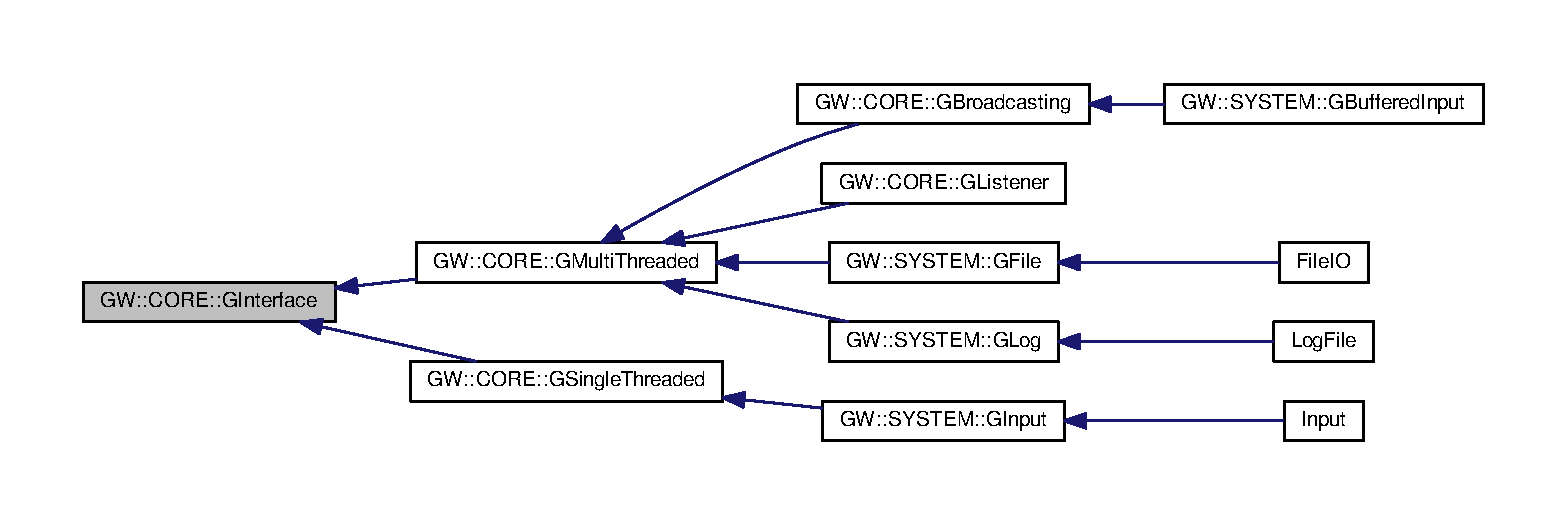
\includegraphics[width=350pt]{classGW_1_1CORE_1_1GInterface__inherit__graph}
\end{center}
\end{figure}
\subsection*{Public Member Functions}
\begin{DoxyCompactItemize}
\item 
virtual \hyperlink{namespaceGW_a67a839e3df7ea8a5c5686613a7a3de21}{G\+Return} \hyperlink{classGW_1_1CORE_1_1GInterface_aacf5834174a7024f8a3c361122ee9e76}{Get\+Count} (unsigned int \&\+\_\+out\+Count)=0
\begin{DoxyCompactList}\small\item\em Return the total number of active references to this object. \end{DoxyCompactList}\item 
virtual \hyperlink{namespaceGW_a67a839e3df7ea8a5c5686613a7a3de21}{G\+Return} \hyperlink{classGW_1_1CORE_1_1GInterface_a2d710f20bb78e544e8309b5b75c21260}{Increment\+Count} ()=0
\begin{DoxyCompactList}\small\item\em Increase the total number of active references to this object. \end{DoxyCompactList}\item 
virtual \hyperlink{namespaceGW_a67a839e3df7ea8a5c5686613a7a3de21}{G\+Return} \hyperlink{classGW_1_1CORE_1_1GInterface_a19a368c77ad0aa7f49b5a4f772f173ba}{Decrement\+Count} ()=0
\begin{DoxyCompactList}\small\item\em Decrease the total number of active references to this object. \end{DoxyCompactList}\item 
virtual \hyperlink{namespaceGW_a67a839e3df7ea8a5c5686613a7a3de21}{G\+Return} \hyperlink{classGW_1_1CORE_1_1GInterface_ad6c8324970172784964f484686d4fdad}{Request\+Interface} (const \hyperlink{structGW_1_1GUUIID}{G\+U\+U\+I\+ID} \&\+\_\+interface\+ID, void $\ast$$\ast$\+\_\+output\+Interface)=0
\begin{DoxyCompactList}\small\item\em Requests an interface that may or may not be supported by this object. \end{DoxyCompactList}\end{DoxyCompactItemize}


\subsection{Detailed Description}
Base interface all Gateware interfaces must support at a minimum. 

Core features include\+: Interface Upgrades, Reference Counting, Event Broadcasting. 

\subsection{Member Function Documentation}
\index{G\+W\+::\+C\+O\+R\+E\+::\+G\+Interface@{G\+W\+::\+C\+O\+R\+E\+::\+G\+Interface}!Decrement\+Count@{Decrement\+Count}}
\index{Decrement\+Count@{Decrement\+Count}!G\+W\+::\+C\+O\+R\+E\+::\+G\+Interface@{G\+W\+::\+C\+O\+R\+E\+::\+G\+Interface}}
\subsubsection[{\texorpdfstring{Decrement\+Count()=0}{DecrementCount()=0}}]{\setlength{\rightskip}{0pt plus 5cm}virtual {\bf G\+Return} G\+W\+::\+C\+O\+R\+E\+::\+G\+Interface\+::\+Decrement\+Count (
\begin{DoxyParamCaption}
{}
\end{DoxyParamCaption}
)\hspace{0.3cm}{\ttfamily [pure virtual]}}\hypertarget{classGW_1_1CORE_1_1GInterface_a19a368c77ad0aa7f49b5a4f772f173ba}{}\label{classGW_1_1CORE_1_1GInterface_a19a368c77ad0aa7f49b5a4f772f173ba}


Decrease the total number of active references to this object. 

Once the internal count reaches zero this object will be deallocated and your pointer will become invalid.


\begin{DoxyRetVals}{Return values}
{\em S\+U\+C\+C\+E\+SS} & Successfully decremented the internal reference count. \\
\hline
{\em F\+A\+I\+L\+U\+RE} & Decrementing of internal reference count would underflow the value. \\
\hline
\end{DoxyRetVals}


Implemented in \hyperlink{classFileIO_ab7e4806ca819c3fcdeeb40a2af5f0298}{File\+IO}, \hyperlink{classLogFile_a555ef35fcdce23ebad05f7dcabaf0757}{Log\+File}, and \hyperlink{classInput_a5c44b3dc2be21c1bad5f32a43a7b7a55}{Input}.

\index{G\+W\+::\+C\+O\+R\+E\+::\+G\+Interface@{G\+W\+::\+C\+O\+R\+E\+::\+G\+Interface}!Get\+Count@{Get\+Count}}
\index{Get\+Count@{Get\+Count}!G\+W\+::\+C\+O\+R\+E\+::\+G\+Interface@{G\+W\+::\+C\+O\+R\+E\+::\+G\+Interface}}
\subsubsection[{\texorpdfstring{Get\+Count(unsigned int \&\+\_\+out\+Count)=0}{GetCount(unsigned int &_outCount)=0}}]{\setlength{\rightskip}{0pt plus 5cm}virtual {\bf G\+Return} G\+W\+::\+C\+O\+R\+E\+::\+G\+Interface\+::\+Get\+Count (
\begin{DoxyParamCaption}
\item[{unsigned int \&}]{\+\_\+out\+Count}
\end{DoxyParamCaption}
)\hspace{0.3cm}{\ttfamily [pure virtual]}}\hypertarget{classGW_1_1CORE_1_1GInterface_aacf5834174a7024f8a3c361122ee9e76}{}\label{classGW_1_1CORE_1_1GInterface_aacf5834174a7024f8a3c361122ee9e76}


Return the total number of active references to this object. 


\begin{DoxyParams}[1]{Parameters}
\mbox{\tt out}  & {\em \+\_\+out\+Count} & The total number of active references of this object.\\
\hline
\end{DoxyParams}

\begin{DoxyRetVals}{Return values}
{\em S\+U\+C\+C\+E\+SS} & Successfully ran. \\
\hline
{\em F\+A\+I\+L\+U\+RE} & Either class does not exist or the internal reference count is corrupt. \\
\hline
\end{DoxyRetVals}


Implemented in \hyperlink{classFileIO_a20566e320ec4cc0d5615bc3bc1fa3013}{File\+IO}, \hyperlink{classLogFile_ab2abbdb01e2b904f112e5e7b20c59a81}{Log\+File}, and \hyperlink{classInput_a2fd6659ae76357836c4c9b3e7070ffb0}{Input}.

\index{G\+W\+::\+C\+O\+R\+E\+::\+G\+Interface@{G\+W\+::\+C\+O\+R\+E\+::\+G\+Interface}!Increment\+Count@{Increment\+Count}}
\index{Increment\+Count@{Increment\+Count}!G\+W\+::\+C\+O\+R\+E\+::\+G\+Interface@{G\+W\+::\+C\+O\+R\+E\+::\+G\+Interface}}
\subsubsection[{\texorpdfstring{Increment\+Count()=0}{IncrementCount()=0}}]{\setlength{\rightskip}{0pt plus 5cm}virtual {\bf G\+Return} G\+W\+::\+C\+O\+R\+E\+::\+G\+Interface\+::\+Increment\+Count (
\begin{DoxyParamCaption}
{}
\end{DoxyParamCaption}
)\hspace{0.3cm}{\ttfamily [pure virtual]}}\hypertarget{classGW_1_1CORE_1_1GInterface_a2d710f20bb78e544e8309b5b75c21260}{}\label{classGW_1_1CORE_1_1GInterface_a2d710f20bb78e544e8309b5b75c21260}


Increase the total number of active references to this object. 

End users should only call this operation if they are familiar with reference counting behavior.


\begin{DoxyRetVals}{Return values}
{\em S\+U\+C\+C\+E\+SS} & Successfully incremented the internal reference count. \\
\hline
{\em F\+A\+I\+L\+U\+RE} & Incrementation of internal reference count would overflow the value. \\
\hline
\end{DoxyRetVals}


Implemented in \hyperlink{classFileIO_a9f2c9a4d13577e14a2c94b0e9617d80b}{File\+IO}, \hyperlink{classLogFile_aff5871b4f2434b6ca722b89581416da0}{Log\+File}, and \hyperlink{classInput_a3c2103023cbb1fa583f910539bb6cce3}{Input}.

\index{G\+W\+::\+C\+O\+R\+E\+::\+G\+Interface@{G\+W\+::\+C\+O\+R\+E\+::\+G\+Interface}!Request\+Interface@{Request\+Interface}}
\index{Request\+Interface@{Request\+Interface}!G\+W\+::\+C\+O\+R\+E\+::\+G\+Interface@{G\+W\+::\+C\+O\+R\+E\+::\+G\+Interface}}
\subsubsection[{\texorpdfstring{Request\+Interface(const G\+U\+U\+I\+I\+D \&\+\_\+interface\+I\+D, void $\ast$$\ast$\+\_\+output\+Interface)=0}{RequestInterface(const GUUIID &_interfaceID, void **_outputInterface)=0}}]{\setlength{\rightskip}{0pt plus 5cm}virtual {\bf G\+Return} G\+W\+::\+C\+O\+R\+E\+::\+G\+Interface\+::\+Request\+Interface (
\begin{DoxyParamCaption}
\item[{const {\bf G\+U\+U\+I\+ID} \&}]{\+\_\+interface\+ID, }
\item[{void $\ast$$\ast$}]{\+\_\+output\+Interface}
\end{DoxyParamCaption}
)\hspace{0.3cm}{\ttfamily [pure virtual]}}\hypertarget{classGW_1_1CORE_1_1GInterface_ad6c8324970172784964f484686d4fdad}{}\label{classGW_1_1CORE_1_1GInterface_ad6c8324970172784964f484686d4fdad}


Requests an interface that may or may not be supported by this object. 

Can be used by the end-\/user to query for a new interface using the unique ID of the interface they want and implement an interface update.


\begin{DoxyParams}[1]{Parameters}
\mbox{\tt in}  & {\em \+\_\+interface\+ID} & The \hyperlink{structGW_1_1GUUIID}{G\+U\+U\+I\+ID} of the interface you are requesting. \\
\hline
\mbox{\tt out}  & {\em \+\_\+output\+Interface} & Where the interface will be stored if function is successful.\\
\hline
\end{DoxyParams}

\begin{DoxyRetVals}{Return values}
{\em S\+U\+C\+C\+E\+SS} & The interface is supported and function succeded. \\
\hline
{\em I\+N\+T\+E\+R\+F\+A\+C\+E\+\_\+\+U\+N\+S\+U\+P\+P\+O\+R\+T\+ED} & The requested interface is not supported. \\
\hline
\end{DoxyRetVals}


Implemented in \hyperlink{classFileIO_a3fb39527fac479474c6ef5045dbc1551}{File\+IO}, \hyperlink{classLogFile_a8b8e63b9c62846b1b9e0cf8b79429ba5}{Log\+File}, and \hyperlink{classInput_a29f3c56e9fec9f9073c1e18f120a69cd}{Input}.



The documentation for this class was generated from the following file\+:\begin{DoxyCompactItemize}
\item 
Interface/\+G\+\_\+\+Core/G\+Interface.\+h\end{DoxyCompactItemize}

\hypertarget{interfaceGIResponder}{}\section{G\+I\+Responder Class Reference}
\label{interfaceGIResponder}\index{G\+I\+Responder@{G\+I\+Responder}}


Inheritance diagram for G\+I\+Responder\+:
\nopagebreak
\begin{figure}[H]
\begin{center}
\leavevmode
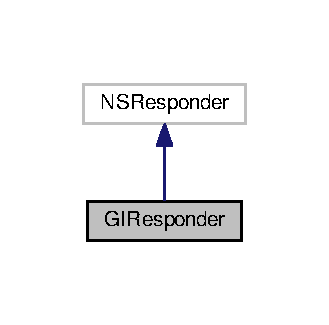
\includegraphics[width=158pt]{interfaceGIResponder__inherit__graph}
\end{center}
\end{figure}


Collaboration diagram for G\+I\+Responder\+:
\nopagebreak
\begin{figure}[H]
\begin{center}
\leavevmode
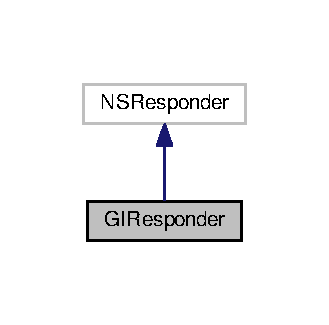
\includegraphics[width=158pt]{interfaceGIResponder__coll__graph}
\end{center}
\end{figure}
\subsection*{Instance Methods}
\begin{DoxyCompactItemize}
\item 
(bool) -\/ {\bfseries accept\+First\+Responder}\hypertarget{interfaceGIResponder_a69336360b238bdbdc953846ffd8ec680}{}\label{interfaceGIResponder_a69336360b238bdbdc953846ffd8ec680}

\item 
(bool) -\/ {\bfseries accepts\+First\+Mouse\+:}\hypertarget{interfaceGIResponder_a7c7a4084b23e4fbbdf87d1aef1aef090}{}\label{interfaceGIResponder_a7c7a4084b23e4fbbdf87d1aef1aef090}

\item 
(void) -\/ {\bfseries key\+Down\+:}\hypertarget{interfaceGIResponder_a4cabb99dc9bb76c07c5528881f7ca9ef}{}\label{interfaceGIResponder_a4cabb99dc9bb76c07c5528881f7ca9ef}

\item 
(void) -\/ {\bfseries key\+Up\+:}\hypertarget{interfaceGIResponder_a2a3be3ad8c5f0bc96b0f4d0006f69581}{}\label{interfaceGIResponder_a2a3be3ad8c5f0bc96b0f4d0006f69581}

\item 
(void) -\/ {\bfseries mouse\+Down\+:}\hypertarget{interfaceGIResponder_a177aff5b20126cb7968706cbb81195c2}{}\label{interfaceGIResponder_a177aff5b20126cb7968706cbb81195c2}

\item 
(void) -\/ {\bfseries mouse\+Up\+:}\hypertarget{interfaceGIResponder_a95d3d4ce7947363452eab0e158e9ebef}{}\label{interfaceGIResponder_a95d3d4ce7947363452eab0e158e9ebef}

\item 
(void) -\/ {\bfseries rightmouse\+Down\+:}\hypertarget{interfaceGIResponder_a51426c29065c07f9e2afbbc8181d6b74}{}\label{interfaceGIResponder_a51426c29065c07f9e2afbbc8181d6b74}

\item 
(void) -\/ {\bfseries rightmouse\+Up\+:}\hypertarget{interfaceGIResponder_abe9b61c47fa25f70ab6a82417979b3b7}{}\label{interfaceGIResponder_abe9b61c47fa25f70ab6a82417979b3b7}

\item 
(void) -\/ {\bfseries othermouse\+Down\+:}\hypertarget{interfaceGIResponder_a4796bfaa60025ff0631b525fd52b2182}{}\label{interfaceGIResponder_a4796bfaa60025ff0631b525fd52b2182}

\item 
(void) -\/ {\bfseries othermouse\+Up\+:}\hypertarget{interfaceGIResponder_a88e82a046893b9aab9f0776173ba6ee8}{}\label{interfaceGIResponder_a88e82a046893b9aab9f0776173ba6ee8}

\item 
(void) -\/ {\bfseries mouse\+Moved\+:}\hypertarget{interfaceGIResponder_a699c6208ac80a3c6d3c4abb222a03a10}{}\label{interfaceGIResponder_a699c6208ac80a3c6d3c4abb222a03a10}

\item 
(void) -\/ {\bfseries Get\+Key\+Mask\+:}\hypertarget{interfaceGIResponder_a060835ad8e859fca137acaee50593a47}{}\label{interfaceGIResponder_a060835ad8e859fca137acaee50593a47}

\end{DoxyCompactItemize}
\subsection*{Protected Attributes}
\begin{DoxyCompactItemize}
\item 
N\+S\+U\+Integer {\bfseries flags}\hypertarget{interfaceGIResponder_acbb29dd4a78a53d141da79b551fc82a5}{}\label{interfaceGIResponder_acbb29dd4a78a53d141da79b551fc82a5}

\end{DoxyCompactItemize}


The documentation for this class was generated from the following file\+:\begin{DoxyCompactItemize}
\item 
Source/\+G\+\_\+\+System/G\+Input.\+mm\end{DoxyCompactItemize}

\hypertarget{classGW_1_1CORE_1_1GListener}{}\section{GW\+::C\+O\+RE\+::G\+Listener Class Reference}
\label{classGW_1_1CORE_1_1GListener}\index{GW::CORE::GListener@{GW::CORE::GListener}}


A \mbox{\hyperlink{classGW_1_1CORE_1_1GListener}{G\+Listener}} Interface may be registered with a G\+Broadcaster interface to receive event notifications.  




{\ttfamily \#include $<$G\+Listener.\+h$>$}



Inheritance diagram for GW\+::C\+O\+RE\+::G\+Listener\+:
% FIG 0


Collaboration diagram for GW\+::C\+O\+RE\+::G\+Listener\+:
% FIG 1
\subsection*{Public Member Functions}
\begin{DoxyCompactItemize}
\item 
virtual \mbox{\hyperlink{namespaceGW_a67a839e3df7ea8a5c5686613a7a3de21}{G\+Return}} \mbox{\hyperlink{classGW_1_1CORE_1_1GListener_a5c1d1fac213b7a1cc15d384aa0c33105}{On\+Event}} (const \mbox{\hyperlink{structGW_1_1GUUIID}{G\+U\+U\+I\+ID}} \&\+\_\+sender\+Interface, unsigned int \+\_\+event\+ID, void $\ast$\+\_\+event\+Data, unsigned int \+\_\+data\+Size)=0
\begin{DoxyCompactList}\small\item\em This operation is called whenever a G\+Broadcaster a listener is registered to generates an event. \end{DoxyCompactList}\end{DoxyCompactItemize}


\subsection{Detailed Description}
A \mbox{\hyperlink{classGW_1_1CORE_1_1GListener}{G\+Listener}} Interface may be registered with a G\+Broadcaster interface to receive event notifications. 

\mbox{\hyperlink{classGW_1_1CORE_1_1GListener}{G\+Listener}} is directly inherited from \mbox{\hyperlink{classGW_1_1CORE_1_1GMultiThreaded}{G\+Multi\+Threaded}}, therefore its implementation must be thread safe. 

\subsection{Member Function Documentation}
\mbox{\Hypertarget{classGW_1_1CORE_1_1GListener_a5c1d1fac213b7a1cc15d384aa0c33105}\label{classGW_1_1CORE_1_1GListener_a5c1d1fac213b7a1cc15d384aa0c33105}} 
\index{GW::CORE::GListener@{GW::CORE::GListener}!OnEvent@{OnEvent}}
\index{OnEvent@{OnEvent}!GW::CORE::GListener@{GW::CORE::GListener}}
\subsubsection{\texorpdfstring{OnEvent()}{OnEvent()}}
{\footnotesize\ttfamily virtual \mbox{\hyperlink{namespaceGW_a67a839e3df7ea8a5c5686613a7a3de21}{G\+Return}} G\+W\+::\+C\+O\+R\+E\+::\+G\+Listener\+::\+On\+Event (\begin{DoxyParamCaption}\item[{const \mbox{\hyperlink{structGW_1_1GUUIID}{G\+U\+U\+I\+ID}} \&}]{\+\_\+sender\+Interface,  }\item[{unsigned int}]{\+\_\+event\+ID,  }\item[{void $\ast$}]{\+\_\+event\+Data,  }\item[{unsigned int}]{\+\_\+data\+Size }\end{DoxyParamCaption})\hspace{0.3cm}{\ttfamily [pure virtual]}}



This operation is called whenever a G\+Broadcaster a listener is registered to generates an event. 


\begin{DoxyParams}[1]{Parameters}
\mbox{\texttt{ in}}  & {\em \+\_\+sender\+Interface} & The interface of the sender object. \\
\hline
\mbox{\texttt{ in}}  & {\em \+\_\+event\+ID} & The ID of the event sent. \\
\hline
\mbox{\texttt{ in}}  & {\em \+\_\+event\+Data} & The data of the event. \\
\hline
\mbox{\texttt{ in}}  & {\em \+\_\+data\+Size} & The size of \+\_\+event\+Data in bytes. \\
\hline
\end{DoxyParams}


The documentation for this class was generated from the following file\+:\begin{DoxyCompactItemize}
\item 
Interface/\+G\+\_\+\+Core/G\+Listener.\+h\end{DoxyCompactItemize}

\hypertarget{classGW_1_1SYSTEM_1_1GLog}{}\section{GW\+:\+:S\+Y\+S\+T\+EM\+:\+:G\+Log Class Reference}
\label{classGW_1_1SYSTEM_1_1GLog}\index{G\+W\+::\+S\+Y\+S\+T\+E\+M\+::\+G\+Log@{G\+W\+::\+S\+Y\+S\+T\+E\+M\+::\+G\+Log}}


Cross platform threadsafe logger.  




{\ttfamily \#include $<$G\+Log.\+h$>$}



Inheritance diagram for GW\+:\+:S\+Y\+S\+T\+EM\+:\+:G\+Log\+:
\nopagebreak
\begin{figure}[H]
\begin{center}
\leavevmode
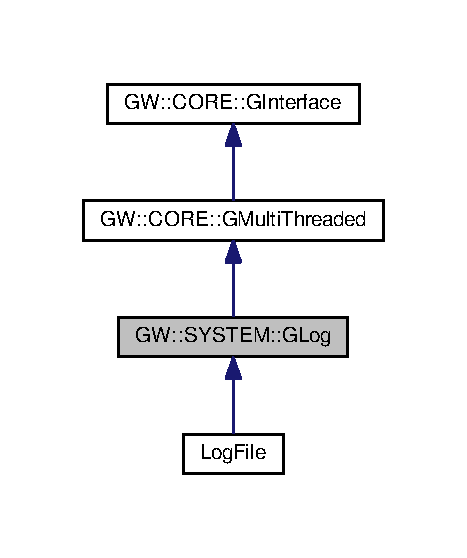
\includegraphics[width=224pt]{classGW_1_1SYSTEM_1_1GLog__inherit__graph}
\end{center}
\end{figure}


Collaboration diagram for GW\+:\+:S\+Y\+S\+T\+EM\+:\+:G\+Log\+:
\nopagebreak
\begin{figure}[H]
\begin{center}
\leavevmode
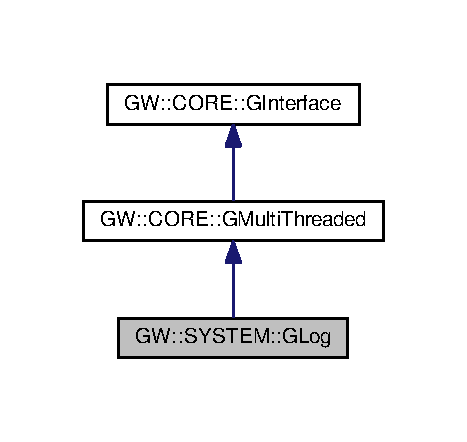
\includegraphics[width=224pt]{classGW_1_1SYSTEM_1_1GLog__coll__graph}
\end{center}
\end{figure}
\subsection*{Public Member Functions}
\begin{DoxyCompactItemize}
\item 
virtual \hyperlink{namespaceGW_a67a839e3df7ea8a5c5686613a7a3de21}{G\+Return} \hyperlink{classGW_1_1SYSTEM_1_1GLog_a9e21e702d012065fe799b4c49f7ac670}{Log} (const char $\ast$const \+\_\+log)=0
\begin{DoxyCompactList}\small\item\em Logs a null terminated string. \end{DoxyCompactList}\item 
virtual \hyperlink{namespaceGW_a67a839e3df7ea8a5c5686613a7a3de21}{G\+Return} \hyperlink{classGW_1_1SYSTEM_1_1GLog_a5d10397fa6aeeebaf8430df6029ec3c5}{Log\+Catergorized} (const char $\ast$const \+\_\+category, const char $\ast$const \+\_\+log)=0
\begin{DoxyCompactList}\small\item\em Logs a null terminated string with a category. \end{DoxyCompactList}\item 
virtual void \hyperlink{classGW_1_1SYSTEM_1_1GLog_a4323c96541a34fb0344828a1c20ec254}{Enable\+Verbose\+Logging} (bool \+\_\+value)=0
\begin{DoxyCompactList}\small\item\em Turns verbose logging on or off. \end{DoxyCompactList}\item 
virtual void \hyperlink{classGW_1_1SYSTEM_1_1GLog_abceb9fdf502b11f2fe72de5edd8f187d}{Enable\+Console\+Logging} (bool \+\_\+value)=0
\begin{DoxyCompactList}\small\item\em Turns console logging on or off. \end{DoxyCompactList}\item 
virtual \hyperlink{namespaceGW_a67a839e3df7ea8a5c5686613a7a3de21}{G\+Return} \hyperlink{classGW_1_1SYSTEM_1_1GLog_a07147c15ecb17caa1c83974b3c54f7d4}{Flush} ()=0
\begin{DoxyCompactList}\small\item\em Forces a log dump to file. \end{DoxyCompactList}\end{DoxyCompactItemize}


\subsection{Detailed Description}
Cross platform threadsafe logger. 

\hyperlink{classGW_1_1SYSTEM_1_1GLog}{G\+Log} inherits directly from G\+Multi\+Threaded, therefore its implementation must be thread safe. 

\subsection{Member Function Documentation}
\index{G\+W\+::\+S\+Y\+S\+T\+E\+M\+::\+G\+Log@{G\+W\+::\+S\+Y\+S\+T\+E\+M\+::\+G\+Log}!Enable\+Console\+Logging@{Enable\+Console\+Logging}}
\index{Enable\+Console\+Logging@{Enable\+Console\+Logging}!G\+W\+::\+S\+Y\+S\+T\+E\+M\+::\+G\+Log@{G\+W\+::\+S\+Y\+S\+T\+E\+M\+::\+G\+Log}}
\subsubsection[{\texorpdfstring{Enable\+Console\+Logging(bool \+\_\+value)=0}{EnableConsoleLogging(bool _value)=0}}]{\setlength{\rightskip}{0pt plus 5cm}virtual void G\+W\+::\+S\+Y\+S\+T\+E\+M\+::\+G\+Log\+::\+Enable\+Console\+Logging (
\begin{DoxyParamCaption}
\item[{bool}]{\+\_\+value}
\end{DoxyParamCaption}
)\hspace{0.3cm}{\ttfamily [pure virtual]}}\hypertarget{classGW_1_1SYSTEM_1_1GLog_abceb9fdf502b11f2fe72de5edd8f187d}{}\label{classGW_1_1SYSTEM_1_1GLog_abceb9fdf502b11f2fe72de5edd8f187d}


Turns console logging on or off. 

Use this function to ensure or prevent the additional console logging.


\begin{DoxyParams}[1]{Parameters}
\mbox{\tt in}  & {\em \+\_\+value} & true to turn on or false to turn off. \\
\hline
\end{DoxyParams}


Implemented in \hyperlink{classLogFile_a903b31947e1c100309dcc5b20548262c}{Log\+File}.

\index{G\+W\+::\+S\+Y\+S\+T\+E\+M\+::\+G\+Log@{G\+W\+::\+S\+Y\+S\+T\+E\+M\+::\+G\+Log}!Enable\+Verbose\+Logging@{Enable\+Verbose\+Logging}}
\index{Enable\+Verbose\+Logging@{Enable\+Verbose\+Logging}!G\+W\+::\+S\+Y\+S\+T\+E\+M\+::\+G\+Log@{G\+W\+::\+S\+Y\+S\+T\+E\+M\+::\+G\+Log}}
\subsubsection[{\texorpdfstring{Enable\+Verbose\+Logging(bool \+\_\+value)=0}{EnableVerboseLogging(bool _value)=0}}]{\setlength{\rightskip}{0pt plus 5cm}virtual void G\+W\+::\+S\+Y\+S\+T\+E\+M\+::\+G\+Log\+::\+Enable\+Verbose\+Logging (
\begin{DoxyParamCaption}
\item[{bool}]{\+\_\+value}
\end{DoxyParamCaption}
)\hspace{0.3cm}{\ttfamily [pure virtual]}}\hypertarget{classGW_1_1SYSTEM_1_1GLog_a4323c96541a34fb0344828a1c20ec254}{}\label{classGW_1_1SYSTEM_1_1GLog_a4323c96541a34fb0344828a1c20ec254}


Turns verbose logging on or off. 

Use this function to ensure or prevent the addition of date, time, and thread\+ID to your log messages.


\begin{DoxyParams}[1]{Parameters}
\mbox{\tt in}  & {\em \+\_\+value} & true to turn on or false to turn off. \\
\hline
\end{DoxyParams}


Implemented in \hyperlink{classLogFile_a250bcfaccded12f7da9a06b6f6336fa5}{Log\+File}.

\index{G\+W\+::\+S\+Y\+S\+T\+E\+M\+::\+G\+Log@{G\+W\+::\+S\+Y\+S\+T\+E\+M\+::\+G\+Log}!Flush@{Flush}}
\index{Flush@{Flush}!G\+W\+::\+S\+Y\+S\+T\+E\+M\+::\+G\+Log@{G\+W\+::\+S\+Y\+S\+T\+E\+M\+::\+G\+Log}}
\subsubsection[{\texorpdfstring{Flush()=0}{Flush()=0}}]{\setlength{\rightskip}{0pt plus 5cm}virtual {\bf G\+Return} G\+W\+::\+S\+Y\+S\+T\+E\+M\+::\+G\+Log\+::\+Flush (
\begin{DoxyParamCaption}
{}
\end{DoxyParamCaption}
)\hspace{0.3cm}{\ttfamily [pure virtual]}}\hypertarget{classGW_1_1SYSTEM_1_1GLog_a07147c15ecb17caa1c83974b3c54f7d4}{}\label{classGW_1_1SYSTEM_1_1GLog_a07147c15ecb17caa1c83974b3c54f7d4}


Forces a log dump to file. 

This will force a log dump to the file and clear the log queue.


\begin{DoxyRetVals}{Return values}
{\em S\+U\+C\+C\+E\+SS} & Successfully dumped the logs. \\
\hline
{\em F\+A\+I\+L\+U\+RE} & Most likely a file corruption or a file is not open. \\
\hline
\end{DoxyRetVals}


Implemented in \hyperlink{classLogFile_a47ffb41f72625b1c7865ac2cd58dea18}{Log\+File}.

\index{G\+W\+::\+S\+Y\+S\+T\+E\+M\+::\+G\+Log@{G\+W\+::\+S\+Y\+S\+T\+E\+M\+::\+G\+Log}!Log@{Log}}
\index{Log@{Log}!G\+W\+::\+S\+Y\+S\+T\+E\+M\+::\+G\+Log@{G\+W\+::\+S\+Y\+S\+T\+E\+M\+::\+G\+Log}}
\subsubsection[{\texorpdfstring{Log(const char $\ast$const \+\_\+log)=0}{Log(const char *const _log)=0}}]{\setlength{\rightskip}{0pt plus 5cm}virtual {\bf G\+Return} G\+W\+::\+S\+Y\+S\+T\+E\+M\+::\+G\+Log\+::\+Log (
\begin{DoxyParamCaption}
\item[{const char $\ast$const}]{\+\_\+log}
\end{DoxyParamCaption}
)\hspace{0.3cm}{\ttfamily [pure virtual]}}\hypertarget{classGW_1_1SYSTEM_1_1GLog_a9e21e702d012065fe799b4c49f7ac670}{}\label{classGW_1_1SYSTEM_1_1GLog_a9e21e702d012065fe799b4c49f7ac670}


Logs a null terminated string. 

Date, Time, and thread ID will be appended to the front of the message unless specified otherwise (See Enable\+Verbose\+Logging). A new line character will be appended to the end of the string so your log messages do not require a new line. The string is logged to the internal \hyperlink{classGW_1_1SYSTEM_1_1GFile}{G\+File} object.


\begin{DoxyParams}[1]{Parameters}
\mbox{\tt in}  & {\em \+\_\+log} & The message to log out.\\
\hline
\end{DoxyParams}

\begin{DoxyRetVals}{Return values}
{\em S\+U\+C\+C\+E\+SS} & Successfully queued the message to the log. \\
\hline
{\em F\+A\+I\+L\+U\+RE} & The queue has reached maximum size (call flush). \\
\hline
{\em I\+N\+V\+A\+L\+I\+D\+\_\+\+A\+R\+G\+U\+M\+E\+NT} & A nullptr was passed in. \\
\hline
\end{DoxyRetVals}


Implemented in \hyperlink{classLogFile_a6848c12fad15f2c835e5215234f75c5a}{Log\+File}.

\index{G\+W\+::\+S\+Y\+S\+T\+E\+M\+::\+G\+Log@{G\+W\+::\+S\+Y\+S\+T\+E\+M\+::\+G\+Log}!Log\+Catergorized@{Log\+Catergorized}}
\index{Log\+Catergorized@{Log\+Catergorized}!G\+W\+::\+S\+Y\+S\+T\+E\+M\+::\+G\+Log@{G\+W\+::\+S\+Y\+S\+T\+E\+M\+::\+G\+Log}}
\subsubsection[{\texorpdfstring{Log\+Catergorized(const char $\ast$const \+\_\+category, const char $\ast$const \+\_\+log)=0}{LogCatergorized(const char *const _category, const char *const _log)=0}}]{\setlength{\rightskip}{0pt plus 5cm}virtual {\bf G\+Return} G\+W\+::\+S\+Y\+S\+T\+E\+M\+::\+G\+Log\+::\+Log\+Catergorized (
\begin{DoxyParamCaption}
\item[{const char $\ast$const}]{\+\_\+category, }
\item[{const char $\ast$const}]{\+\_\+log}
\end{DoxyParamCaption}
)\hspace{0.3cm}{\ttfamily [pure virtual]}}\hypertarget{classGW_1_1SYSTEM_1_1GLog_a5d10397fa6aeeebaf8430df6029ec3c5}{}\label{classGW_1_1SYSTEM_1_1GLog_a5d10397fa6aeeebaf8430df6029ec3c5}


Logs a null terminated string with a category. 

Date, Time, and thread ID will be appended to the front of the message unless specified otherwise (See Enable\+Verbose\+Logging). A new line character will be appended to the end of the string so your log messages do not require a new line. The string is logged to the internal \hyperlink{classGW_1_1SYSTEM_1_1GFile}{G\+File} object.


\begin{DoxyParams}[1]{Parameters}
\mbox{\tt in}  & {\em \+\_\+category} & The category the log belongs in. ie. E\+R\+R\+OR, W\+A\+R\+N\+I\+NG, I\+N\+FO, etc. \\
\hline
\mbox{\tt in}  & {\em \+\_\+log} & The message to log out.\\
\hline
\end{DoxyParams}

\begin{DoxyRetVals}{Return values}
{\em S\+U\+C\+C\+E\+SS} & Successfully queued the message to the log. \\
\hline
{\em F\+A\+I\+L\+U\+RE} & The queue has reached maximum size (call flush). \\
\hline
{\em I\+N\+V\+A\+L\+I\+D\+\_\+\+A\+R\+G\+U\+M\+E\+NT} & Either \+\_\+category or \+\_\+log are nullptr. \\
\hline
\end{DoxyRetVals}


Implemented in \hyperlink{classLogFile_a5e5f24ccd4c6f925dd8bc1ced512b530}{Log\+File}.



The documentation for this class was generated from the following file\+:\begin{DoxyCompactItemize}
\item 
Interface/\+G\+\_\+\+System/G\+Log.\+h\end{DoxyCompactItemize}

\hypertarget{classGW_1_1CORE_1_1GMultiThreaded}{}\section{GW\+::C\+O\+RE\+::G\+Multi\+Threaded Class Reference}
\label{classGW_1_1CORE_1_1GMultiThreaded}\index{GW::CORE::GMultiThreaded@{GW::CORE::GMultiThreaded}}


This interface is only used to label and query interfaces which promise to 100\% internally support thread safety.  




{\ttfamily \#include $<$G\+Multi\+Threaded.\+h$>$}



Inheritance diagram for GW\+::C\+O\+RE\+::G\+Multi\+Threaded\+:
% FIG 0


Collaboration diagram for GW\+::C\+O\+RE\+::G\+Multi\+Threaded\+:
% FIG 1
\subsection*{Additional Inherited Members}


\subsection{Detailed Description}
This interface is only used to label and query interfaces which promise to 100\% internally support thread safety. 

The documentation for this class was generated from the following file\+:\begin{DoxyCompactItemize}
\item 
Interface/\+G\+\_\+\+Core/G\+Multi\+Threaded.\+h\end{DoxyCompactItemize}

\hypertarget{interfaceGResponder}{}\section{G\+Responder Class Reference}
\label{interfaceGResponder}\index{G\+Responder@{G\+Responder}}


Inheritance diagram for G\+Responder\+:
\nopagebreak
\begin{figure}[H]
\begin{center}
\leavevmode
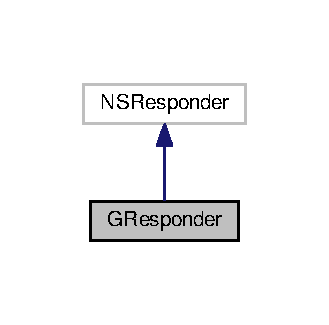
\includegraphics[width=158pt]{interfaceGResponder__inherit__graph}
\end{center}
\end{figure}


Collaboration diagram for G\+Responder\+:
\nopagebreak
\begin{figure}[H]
\begin{center}
\leavevmode
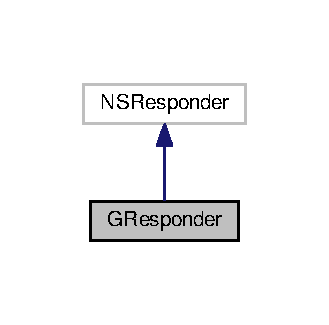
\includegraphics[width=158pt]{interfaceGResponder__coll__graph}
\end{center}
\end{figure}
\subsection*{Instance Methods}
\begin{DoxyCompactItemize}
\item 
(bool) -\/ {\bfseries accept\+First\+Responder}\hypertarget{interfaceGResponder_a38d089c6fa50dadb001917d4376136c5}{}\label{interfaceGResponder_a38d089c6fa50dadb001917d4376136c5}

\item 
(bool) -\/ {\bfseries accepts\+First\+Mouse\+:}\hypertarget{interfaceGResponder_a9358ee727560f1a9fa05b063051bf425}{}\label{interfaceGResponder_a9358ee727560f1a9fa05b063051bf425}

\item 
(void) -\/ {\bfseries key\+Down\+:}\hypertarget{interfaceGResponder_a546f385e994c7eb9fcf16a244c0ecef6}{}\label{interfaceGResponder_a546f385e994c7eb9fcf16a244c0ecef6}

\item 
(void) -\/ {\bfseries key\+Up\+:}\hypertarget{interfaceGResponder_a6474d631363b8835109a5d0934aa84bf}{}\label{interfaceGResponder_a6474d631363b8835109a5d0934aa84bf}

\item 
(void) -\/ {\bfseries mouse\+Down\+:}\hypertarget{interfaceGResponder_ae5fe08f8848c8ee139da21ebac0b2204}{}\label{interfaceGResponder_ae5fe08f8848c8ee139da21ebac0b2204}

\item 
(void) -\/ {\bfseries mouse\+Up\+:}\hypertarget{interfaceGResponder_aebc62bc4faf4cf99635a1481eca99004}{}\label{interfaceGResponder_aebc62bc4faf4cf99635a1481eca99004}

\item 
(void) -\/ {\bfseries rightmouse\+Down\+:}\hypertarget{interfaceGResponder_a25f874602d27e9e8c8601e3524bee880}{}\label{interfaceGResponder_a25f874602d27e9e8c8601e3524bee880}

\item 
(void) -\/ {\bfseries rightmouse\+Up\+:}\hypertarget{interfaceGResponder_a20a0b3baac9815710c7d62f1df1d9165}{}\label{interfaceGResponder_a20a0b3baac9815710c7d62f1df1d9165}

\item 
(void) -\/ {\bfseries othermouse\+Down\+:}\hypertarget{interfaceGResponder_a47a3c5d341c5d5066ab91b2e0746b438}{}\label{interfaceGResponder_a47a3c5d341c5d5066ab91b2e0746b438}

\item 
(void) -\/ {\bfseries othermouse\+Up\+:}\hypertarget{interfaceGResponder_a8e07cdcdc82a14526a6b0ebf1b1db458}{}\label{interfaceGResponder_a8e07cdcdc82a14526a6b0ebf1b1db458}

\item 
(void) -\/ {\bfseries scroll\+Wheel\+:}\hypertarget{interfaceGResponder_af419f86d1634b577f9749a3ad0bf2040}{}\label{interfaceGResponder_af419f86d1634b577f9749a3ad0bf2040}

\item 
(void) -\/ {\bfseries Get\+Key\+Mask\+:}\hypertarget{interfaceGResponder_ae59e6d264d257ca2c6068f6dd861ae8c}{}\label{interfaceGResponder_ae59e6d264d257ca2c6068f6dd861ae8c}

\end{DoxyCompactItemize}


The documentation for this class was generated from the following file\+:\begin{DoxyCompactItemize}
\item 
Source/\+G\+\_\+\+System/G\+Buffered\+Input.\+mm\end{DoxyCompactItemize}

\hypertarget{classGW_1_1CORE_1_1GSingleThreaded}{}\section{GW\+::C\+O\+RE\+::G\+Single\+Threaded Class Reference}
\label{classGW_1_1CORE_1_1GSingleThreaded}\index{GW::CORE::GSingleThreaded@{GW::CORE::GSingleThreaded}}


This interface is only used to label and query interfaces which are not designed internally to support thread safety.  




{\ttfamily \#include $<$G\+Single\+Threaded.\+h$>$}



Inheritance diagram for GW\+::C\+O\+RE\+::G\+Single\+Threaded\+:
% FIG 0


Collaboration diagram for GW\+::C\+O\+RE\+::G\+Single\+Threaded\+:
% FIG 1
\subsection*{Additional Inherited Members}


\subsection{Detailed Description}
This interface is only used to label and query interfaces which are not designed internally to support thread safety. 

The documentation for this class was generated from the following file\+:\begin{DoxyCompactItemize}
\item 
Interface/\+G\+\_\+\+Core/G\+Single\+Threaded.\+h\end{DoxyCompactItemize}

\hypertarget{structGW_1_1GUUIID}{}\section{GW\+:\+:G\+U\+U\+I\+ID Struct Reference}
\label{structGW_1_1GUUIID}\index{G\+W\+::\+G\+U\+U\+I\+ID@{G\+W\+::\+G\+U\+U\+I\+ID}}


Gateware Universally Unique Interface I\+Dentifier.  




{\ttfamily \#include $<$G\+Defines.\+h$>$}

\subsection*{Public Member Functions}
\begin{DoxyCompactItemize}
\item 
bool \hyperlink{structGW_1_1GUUIID_a84e8d2cc912c79229af8dd9a898e1ace}{operator==} (const \hyperlink{structGW_1_1GUUIID}{G\+U\+U\+I\+ID} \&\+\_\+cmp) const \hypertarget{structGW_1_1GUUIID_a84e8d2cc912c79229af8dd9a898e1ace}{}\label{structGW_1_1GUUIID_a84e8d2cc912c79229af8dd9a898e1ace}

\begin{DoxyCompactList}\small\item\em Comparison operator overload. \end{DoxyCompactList}\end{DoxyCompactItemize}
\subsection*{Public Attributes}
\begin{DoxyCompactItemize}
\item 
\begin{tabbing}
xx\=xx\=xx\=xx\=xx\=xx\=xx\=xx\=xx\=\kill
union \{\\
\>struct \{\\
\>\>unsigned int {\bfseries byte4}\\
\>\>unsigned short {\bfseries byte2a}\\
\>\>unsigned short {\bfseries byte2b}\\
\>\>unsigned char {\bfseries byte8} \mbox{[}8\mbox{]}\\
\>\} \hypertarget{unionGW_1_1GUUIID_1_1_0D0_a408b2437c2ea63a4cb75888db0ac62fb}{}\label{unionGW_1_1GUUIID_1_1_0D0_a408b2437c2ea63a4cb75888db0ac62fb}
\\
\>unsigned long long {\bfseries parts} \mbox{[}2\mbox{]}\\
\}; \hypertarget{structGW_1_1GUUIID_aa51f004bf72e52a4e15b7568b9a7ec50}{}\label{structGW_1_1GUUIID_aa51f004bf72e52a4e15b7568b9a7ec50}
\\

\end{tabbing}\end{DoxyCompactItemize}


\subsection{Detailed Description}
Gateware Universally Unique Interface I\+Dentifier. 

Each \hyperlink{structGW_1_1GUUIID}{G\+U\+U\+I\+ID} defines a unique 128bit number identifying a particular version of an interface. This allows interfaces to be upgraded down the line safely without breaking legacy code. 

The documentation for this struct was generated from the following file\+:\begin{DoxyCompactItemize}
\item 
Interface/\+G\+\_\+\+Core/G\+Defines.\+h\end{DoxyCompactItemize}

\hypertarget{classInput}{}\section{Input Class Reference}
\label{classInput}\index{Input@{Input}}


Inheritance diagram for Input\+:
\nopagebreak
\begin{figure}[H]
\begin{center}
\leavevmode
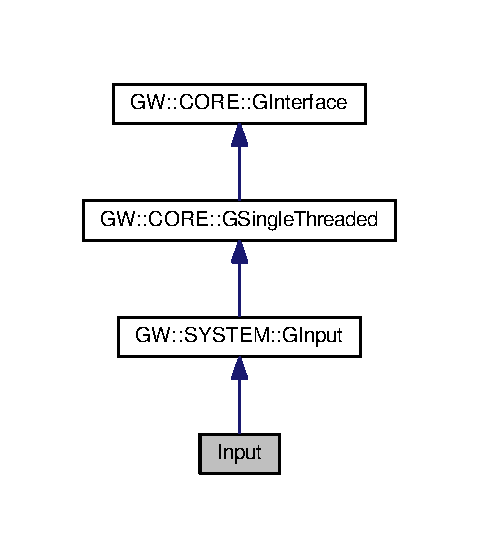
\includegraphics[width=230pt]{classInput__inherit__graph}
\end{center}
\end{figure}


Collaboration diagram for Input\+:
\nopagebreak
\begin{figure}[H]
\begin{center}
\leavevmode
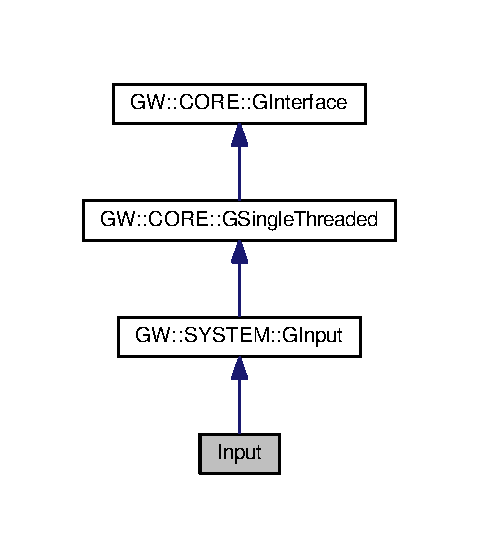
\includegraphics[width=230pt]{classInput__coll__graph}
\end{center}
\end{figure}
\subsection*{Public Member Functions}
\begin{DoxyCompactItemize}
\item 
void {\bfseries Input\+Thread} ()\hypertarget{classInput_a373c67d7fd7e2b81a0f498afb201b124}{}\label{classInput_a373c67d7fd7e2b81a0f498afb201b124}

\item 
\hyperlink{namespaceGW_a67a839e3df7ea8a5c5686613a7a3de21}{G\+Return} {\bfseries Initialize\+Windows} (void $\ast$\+\_\+data)\hypertarget{classInput_a180c021bb7e2e2a77325027f1e79d7fe}{}\label{classInput_a180c021bb7e2e2a77325027f1e79d7fe}

\item 
\hyperlink{namespaceGW_a67a839e3df7ea8a5c5686613a7a3de21}{G\+Return} \hyperlink{classInput_a1d195bdfcab3c160f99b1010face1e61}{Initialize\+Linux} (void $\ast$\+\_\+data)
\item 
\hyperlink{namespaceGW_a67a839e3df7ea8a5c5686613a7a3de21}{G\+Return} {\bfseries Initialize\+Mac} (void $\ast$\+\_\+data)\hypertarget{classInput_ad83dda6b9dd9388be971ff580451cfb9}{}\label{classInput_ad83dda6b9dd9388be971ff580451cfb9}

\item 
float \hyperlink{classInput_a7e468df0f31131f3fbcbc6de87d01ec2}{Get\+State} (int \+\_\+key\+Code, \hyperlink{namespaceGW_a67a839e3df7ea8a5c5686613a7a3de21}{G\+Return} $\ast$\+\_\+error\+Code)
\begin{DoxyCompactList}\small\item\em Get the current state of any key. \end{DoxyCompactList}\item 
\hyperlink{namespaceGW_a67a839e3df7ea8a5c5686613a7a3de21}{G\+Return} \hyperlink{classInput_a82d54ae7aa3ecacebe42480eb0aff985}{Get\+Mouse\+Delta} (float \&\+\_\+x, float \&\+\_\+y)
\begin{DoxyCompactList}\small\item\em Get the change in mouse position. \end{DoxyCompactList}\item 
\hyperlink{namespaceGW_a67a839e3df7ea8a5c5686613a7a3de21}{G\+Return} \hyperlink{classInput_a93d7ab591a1d1e8d619318834c75207a}{Get\+Mouse\+Position} (float \&\+\_\+x, float \&\+\_\+y)
\begin{DoxyCompactList}\small\item\em Get the most recent mouse position. \end{DoxyCompactList}\item 
unsigned int \hyperlink{classInput_a8f9b65ea323da8c25a5e70eb6746d4ab}{Get\+Key\+Mask} ()
\begin{DoxyCompactList}\small\item\em Get the key mask. \end{DoxyCompactList}\item 
\hyperlink{namespaceGW_a67a839e3df7ea8a5c5686613a7a3de21}{G\+Return} \hyperlink{classInput_a2fd6659ae76357836c4c9b3e7070ffb0}{Get\+Count} (unsigned int \&\+\_\+out\+Count)
\begin{DoxyCompactList}\small\item\em Return the total number of active references to this object. \end{DoxyCompactList}\item 
\hyperlink{namespaceGW_a67a839e3df7ea8a5c5686613a7a3de21}{G\+Return} \hyperlink{classInput_a3c2103023cbb1fa583f910539bb6cce3}{Increment\+Count} ()
\begin{DoxyCompactList}\small\item\em Increase the total number of active references to this object. \end{DoxyCompactList}\item 
\hyperlink{namespaceGW_a67a839e3df7ea8a5c5686613a7a3de21}{G\+Return} \hyperlink{classInput_a5c44b3dc2be21c1bad5f32a43a7b7a55}{Decrement\+Count} ()
\begin{DoxyCompactList}\small\item\em Decrease the total number of active references to this object. \end{DoxyCompactList}\item 
\hyperlink{namespaceGW_a67a839e3df7ea8a5c5686613a7a3de21}{G\+Return} \hyperlink{classInput_a29f3c56e9fec9f9073c1e18f120a69cd}{Request\+Interface} (const \hyperlink{structGW_1_1GUUIID}{G\+U\+U\+I\+ID} \&\+\_\+interface\+ID, void $\ast$$\ast$\+\_\+output\+Interface)
\begin{DoxyCompactList}\small\item\em Requests an interface that may or may not be supported by this object. \end{DoxyCompactList}\end{DoxyCompactItemize}


\subsection{Member Function Documentation}
\index{Input@{Input}!Decrement\+Count@{Decrement\+Count}}
\index{Decrement\+Count@{Decrement\+Count}!Input@{Input}}
\subsubsection[{\texorpdfstring{Decrement\+Count()}{DecrementCount()}}]{\setlength{\rightskip}{0pt plus 5cm}{\bf G\+Return} Input\+::\+Decrement\+Count (
\begin{DoxyParamCaption}
{}
\end{DoxyParamCaption}
)\hspace{0.3cm}{\ttfamily [virtual]}}\hypertarget{classInput_a5c44b3dc2be21c1bad5f32a43a7b7a55}{}\label{classInput_a5c44b3dc2be21c1bad5f32a43a7b7a55}


Decrease the total number of active references to this object. 

Once the internal count reaches zero this object will be deallocated and your pointer will become invalid.


\begin{DoxyRetVals}{Return values}
{\em S\+U\+C\+C\+E\+SS} & Successfully decremented the internal reference count. \\
\hline
{\em F\+A\+I\+L\+U\+RE} & Decrementing of internal reference count would underflow the value. \\
\hline
\end{DoxyRetVals}


Implements \hyperlink{classGW_1_1CORE_1_1GInterface_a19a368c77ad0aa7f49b5a4f772f173ba}{G\+W\+::\+C\+O\+R\+E\+::\+G\+Interface}.

\index{Input@{Input}!Get\+Count@{Get\+Count}}
\index{Get\+Count@{Get\+Count}!Input@{Input}}
\subsubsection[{\texorpdfstring{Get\+Count(unsigned int \&\+\_\+out\+Count)}{GetCount(unsigned int &_outCount)}}]{\setlength{\rightskip}{0pt plus 5cm}{\bf G\+Return} Input\+::\+Get\+Count (
\begin{DoxyParamCaption}
\item[{unsigned int \&}]{\+\_\+out\+Count}
\end{DoxyParamCaption}
)\hspace{0.3cm}{\ttfamily [virtual]}}\hypertarget{classInput_a2fd6659ae76357836c4c9b3e7070ffb0}{}\label{classInput_a2fd6659ae76357836c4c9b3e7070ffb0}


Return the total number of active references to this object. 


\begin{DoxyParams}[1]{Parameters}
\mbox{\tt out}  & {\em \+\_\+out\+Count} & The total number of active references of this object.\\
\hline
\end{DoxyParams}

\begin{DoxyRetVals}{Return values}
{\em S\+U\+C\+C\+E\+SS} & Successfully ran. \\
\hline
{\em F\+A\+I\+L\+U\+RE} & Either class does not exist or the internal reference count is corrupt. \\
\hline
\end{DoxyRetVals}


Implements \hyperlink{classGW_1_1CORE_1_1GInterface_aacf5834174a7024f8a3c361122ee9e76}{G\+W\+::\+C\+O\+R\+E\+::\+G\+Interface}.

\index{Input@{Input}!Get\+Key\+Mask@{Get\+Key\+Mask}}
\index{Get\+Key\+Mask@{Get\+Key\+Mask}!Input@{Input}}
\subsubsection[{\texorpdfstring{Get\+Key\+Mask()}{GetKeyMask()}}]{\setlength{\rightskip}{0pt plus 5cm}unsigned int Input\+::\+Get\+Key\+Mask (
\begin{DoxyParamCaption}
{}
\end{DoxyParamCaption}
)\hspace{0.3cm}{\ttfamily [virtual]}}\hypertarget{classInput_a8f9b65ea323da8c25a5e70eb6746d4ab}{}\label{classInput_a8f9b65ea323da8c25a5e70eb6746d4ab}


Get the key mask. 

The key mask lets the input object know which of the functions below are active by manipulating individual bits of an unsigned int.


\begin{DoxyRetVals}{Return values}
{\em G\+\_\+\+M\+A\+SK} & (\+\_\+\+S\+H\+I\+FT, \+\_\+\+C\+O\+N\+T\+R\+OL, \+\_\+\+C\+A\+P\+S\+\_\+\+L\+O\+CK, \+\_\+\+N\+U\+M\+\_\+\+L\+O\+CK, \+\_\+\+S\+C\+R\+O\+L\+L\+\_\+\+L\+O\+CK). \\
\hline
\end{DoxyRetVals}


Implements \hyperlink{classGW_1_1SYSTEM_1_1GInput_a071a399bc9c400f0cd333958d911c8c2}{G\+W\+::\+S\+Y\+S\+T\+E\+M\+::\+G\+Input}.

\index{Input@{Input}!Get\+Mouse\+Delta@{Get\+Mouse\+Delta}}
\index{Get\+Mouse\+Delta@{Get\+Mouse\+Delta}!Input@{Input}}
\subsubsection[{\texorpdfstring{Get\+Mouse\+Delta(float \&\+\_\+x, float \&\+\_\+y)}{GetMouseDelta(float &_x, float &_y)}}]{\setlength{\rightskip}{0pt plus 5cm}{\bf G\+Return} Input\+::\+Get\+Mouse\+Delta (
\begin{DoxyParamCaption}
\item[{float \&}]{x, }
\item[{float \&}]{y}
\end{DoxyParamCaption}
)\hspace{0.3cm}{\ttfamily [virtual]}}\hypertarget{classInput_a82d54ae7aa3ecacebe42480eb0aff985}{}\label{classInput_a82d54ae7aa3ecacebe42480eb0aff985}


Get the change in mouse position. 


\begin{DoxyParams}[1]{Parameters}
\mbox{\tt out}  & {\em x} & a reference to a float to store the mouse delta position x. \\
\hline
\mbox{\tt out}  & {\em y} & a reference to a float to store the mouse delta position y.\\
\hline
\end{DoxyParams}

\begin{DoxyRetVals}{Return values}
{\em S\+U\+C\+C\+E\+SS} & no problems found. Values stored in x and y. \\
\hline
\end{DoxyRetVals}


Implements \hyperlink{classGW_1_1SYSTEM_1_1GInput_a2c968f0195241813dea705fb9a02a8b5}{G\+W\+::\+S\+Y\+S\+T\+E\+M\+::\+G\+Input}.

\index{Input@{Input}!Get\+Mouse\+Position@{Get\+Mouse\+Position}}
\index{Get\+Mouse\+Position@{Get\+Mouse\+Position}!Input@{Input}}
\subsubsection[{\texorpdfstring{Get\+Mouse\+Position(float \&\+\_\+x, float \&\+\_\+y)}{GetMousePosition(float &_x, float &_y)}}]{\setlength{\rightskip}{0pt plus 5cm}{\bf G\+Return} Input\+::\+Get\+Mouse\+Position (
\begin{DoxyParamCaption}
\item[{float \&}]{x, }
\item[{float \&}]{y}
\end{DoxyParamCaption}
)\hspace{0.3cm}{\ttfamily [virtual]}}\hypertarget{classInput_a93d7ab591a1d1e8d619318834c75207a}{}\label{classInput_a93d7ab591a1d1e8d619318834c75207a}


Get the most recent mouse position. 


\begin{DoxyParams}[1]{Parameters}
\mbox{\tt out}  & {\em x} & a reference to a float to store the mouse position x. \\
\hline
\mbox{\tt out}  & {\em y} & a reference to a float to store the mouse position y.\\
\hline
\end{DoxyParams}

\begin{DoxyRetVals}{Return values}
{\em S\+U\+C\+C\+E\+SS} & no problems found. Values stored in x and y. \\
\hline
\end{DoxyRetVals}


Implements \hyperlink{classGW_1_1SYSTEM_1_1GInput_af0d0f1a00a2ebd04d5d697d1468c3c00}{G\+W\+::\+S\+Y\+S\+T\+E\+M\+::\+G\+Input}.

\index{Input@{Input}!Get\+State@{Get\+State}}
\index{Get\+State@{Get\+State}!Input@{Input}}
\subsubsection[{\texorpdfstring{Get\+State(int \+\_\+key\+Code, G\+Return $\ast$\+\_\+error\+Code)}{GetState(int _keyCode, GReturn *_errorCode)}}]{\setlength{\rightskip}{0pt plus 5cm}float Input\+::\+Get\+State (
\begin{DoxyParamCaption}
\item[{int}]{\+\_\+key\+Code, }
\item[{{\bf G\+Return} $\ast$}]{error\+Code}
\end{DoxyParamCaption}
)\hspace{0.3cm}{\ttfamily [virtual]}}\hypertarget{classInput_a7e468df0f31131f3fbcbc6de87d01ec2}{}\label{classInput_a7e468df0f31131f3fbcbc6de87d01ec2}


Get the current state of any key. 

Use keycodes in G\+Key\+Defines as input to this function to check the state of a particular key or button.


\begin{DoxyParams}[1]{Parameters}
\mbox{\tt in}  & {\em \+\_\+key\+Code} & The key code of the key to check. \\
\hline
\mbox{\tt out}  & {\em error\+Code} & If function fails this will hold the error\+Code.\\
\hline
\end{DoxyParams}

\begin{DoxyRetVals}{Return values}
{\em 0} & The Key is not pressed. \\
\hline
{\em 1} & The Key is pressed. \\
\hline
\end{DoxyRetVals}


Implements \hyperlink{classGW_1_1SYSTEM_1_1GInput_a7a3e93a3730d05cfeb92fc1dd93ad07a}{G\+W\+::\+S\+Y\+S\+T\+E\+M\+::\+G\+Input}.

\index{Input@{Input}!Increment\+Count@{Increment\+Count}}
\index{Increment\+Count@{Increment\+Count}!Input@{Input}}
\subsubsection[{\texorpdfstring{Increment\+Count()}{IncrementCount()}}]{\setlength{\rightskip}{0pt plus 5cm}{\bf G\+Return} Input\+::\+Increment\+Count (
\begin{DoxyParamCaption}
{}
\end{DoxyParamCaption}
)\hspace{0.3cm}{\ttfamily [virtual]}}\hypertarget{classInput_a3c2103023cbb1fa583f910539bb6cce3}{}\label{classInput_a3c2103023cbb1fa583f910539bb6cce3}


Increase the total number of active references to this object. 

End users should only call this operation if they are familiar with reference counting behavior.


\begin{DoxyRetVals}{Return values}
{\em S\+U\+C\+C\+E\+SS} & Successfully incremented the internal reference count. \\
\hline
{\em F\+A\+I\+L\+U\+RE} & Incrementation of internal reference count would overflow the value. \\
\hline
\end{DoxyRetVals}


Implements \hyperlink{classGW_1_1CORE_1_1GInterface_a2d710f20bb78e544e8309b5b75c21260}{G\+W\+::\+C\+O\+R\+E\+::\+G\+Interface}.

\index{Input@{Input}!Initialize\+Linux@{Initialize\+Linux}}
\index{Initialize\+Linux@{Initialize\+Linux}!Input@{Input}}
\subsubsection[{\texorpdfstring{Initialize\+Linux(void $\ast$\+\_\+data)}{InitializeLinux(void *_data)}}]{\setlength{\rightskip}{0pt plus 5cm}{\bf G\+Return} Input\+::\+Initialize\+Linux (
\begin{DoxyParamCaption}
\item[{void $\ast$}]{\+\_\+data}
\end{DoxyParamCaption}
)}\hypertarget{classInput_a1d195bdfcab3c160f99b1010face1e61}{}\label{classInput_a1d195bdfcab3c160f99b1010face1e61}
X\+Auto\+Repeat\+Off(\+\_\+display); \index{Input@{Input}!Request\+Interface@{Request\+Interface}}
\index{Request\+Interface@{Request\+Interface}!Input@{Input}}
\subsubsection[{\texorpdfstring{Request\+Interface(const G\+U\+U\+I\+I\+D \&\+\_\+interface\+I\+D, void $\ast$$\ast$\+\_\+output\+Interface)}{RequestInterface(const GUUIID &_interfaceID, void **_outputInterface)}}]{\setlength{\rightskip}{0pt plus 5cm}{\bf G\+Return} Input\+::\+Request\+Interface (
\begin{DoxyParamCaption}
\item[{const {\bf G\+U\+U\+I\+ID} \&}]{\+\_\+interface\+ID, }
\item[{void $\ast$$\ast$}]{\+\_\+output\+Interface}
\end{DoxyParamCaption}
)\hspace{0.3cm}{\ttfamily [virtual]}}\hypertarget{classInput_a29f3c56e9fec9f9073c1e18f120a69cd}{}\label{classInput_a29f3c56e9fec9f9073c1e18f120a69cd}


Requests an interface that may or may not be supported by this object. 

Can be used by the end-\/user to query for a new interface using the unique ID of the interface they want and implement an interface update.


\begin{DoxyParams}[1]{Parameters}
\mbox{\tt in}  & {\em \+\_\+interface\+ID} & The G\+U\+U\+I\+ID of the interface you are requesting. \\
\hline
\mbox{\tt out}  & {\em \+\_\+output\+Interface} & Where the interface will be stored if function is successful.\\
\hline
\end{DoxyParams}

\begin{DoxyRetVals}{Return values}
{\em S\+U\+C\+C\+E\+SS} & The interface is supported and function succeded. \\
\hline
{\em I\+N\+T\+E\+R\+F\+A\+C\+E\+\_\+\+U\+N\+S\+U\+P\+P\+O\+R\+T\+ED} & The requested interface is not supported. \\
\hline
\end{DoxyRetVals}


Implements \hyperlink{classGW_1_1CORE_1_1GInterface_ad6c8324970172784964f484686d4fdad}{G\+W\+::\+C\+O\+R\+E\+::\+G\+Interface}.



The documentation for this class was generated from the following file\+:\begin{DoxyCompactItemize}
\item 
Source/\+G\+\_\+\+System/G\+Input.\+cpp\end{DoxyCompactItemize}

\hypertarget{structGW_1_1SYSTEM_1_1LINUX__WINDOW}{}\section{GW\+::S\+Y\+S\+T\+EM\+::L\+I\+N\+U\+X\+\_\+\+W\+I\+N\+D\+OW Struct Reference}
\label{structGW_1_1SYSTEM_1_1LINUX__WINDOW}\index{GW::SYSTEM::LINUX\_WINDOW@{GW::SYSTEM::LINUX\_WINDOW}}


The structure used to pass into Input libraries on Linux.  




{\ttfamily \#include $<$G\+Key\+Defines.\+h$>$}

\subsection*{Public Attributes}
\begin{DoxyCompactItemize}
\item 
\mbox{\Hypertarget{structGW_1_1SYSTEM_1_1LINUX__WINDOW_a9d4ffe1d048716af5f2d1fe3595b6b99}\label{structGW_1_1SYSTEM_1_1LINUX__WINDOW_a9d4ffe1d048716af5f2d1fe3595b6b99}} 
void $\ast$ {\bfseries window}
\item 
\mbox{\Hypertarget{structGW_1_1SYSTEM_1_1LINUX__WINDOW_ae68b93065e8ebd9de010f42ccf688ac5}\label{structGW_1_1SYSTEM_1_1LINUX__WINDOW_ae68b93065e8ebd9de010f42ccf688ac5}} 
void $\ast$ {\bfseries display}
\end{DoxyCompactItemize}


\subsection{Detailed Description}
The structure used to pass into Input libraries on Linux. 

The documentation for this struct was generated from the following file\+:\begin{DoxyCompactItemize}
\item 
Interface/\+G\+\_\+\+System/G\+Key\+Defines.\+h\end{DoxyCompactItemize}

\hypertarget{classLogFile}{}\section{Log\+File Class Reference}
\label{classLogFile}\index{Log\+File@{Log\+File}}


Inheritance diagram for Log\+File\+:
\nopagebreak
\begin{figure}[H]
\begin{center}
\leavevmode
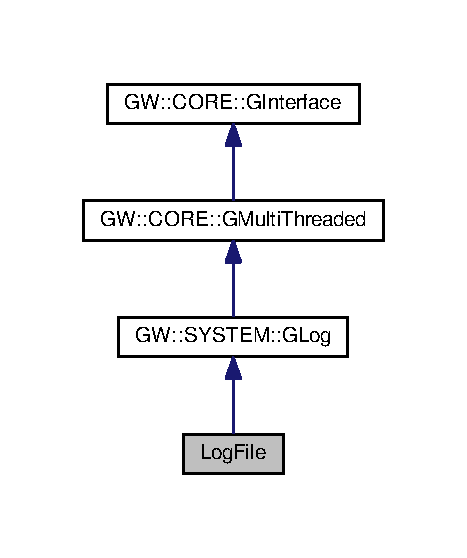
\includegraphics[width=224pt]{classLogFile__inherit__graph}
\end{center}
\end{figure}


Collaboration diagram for Log\+File\+:
\nopagebreak
\begin{figure}[H]
\begin{center}
\leavevmode
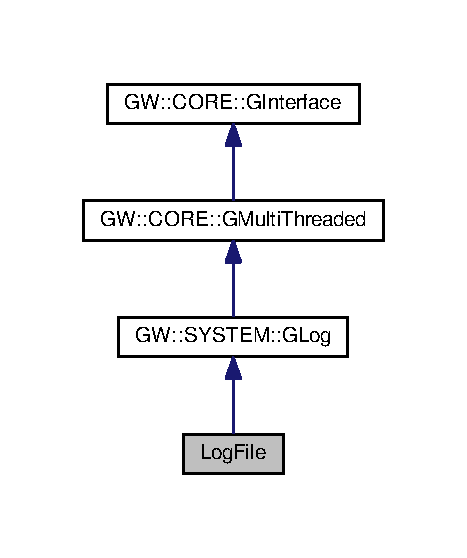
\includegraphics[width=224pt]{classLogFile__coll__graph}
\end{center}
\end{figure}
\subsection*{Public Member Functions}
\begin{DoxyCompactItemize}
\item 
\hyperlink{namespaceGW_a67a839e3df7ea8a5c5686613a7a3de21}{G\+W\+::\+G\+Return} {\bfseries Init} (const char $\ast$const \+\_\+file\+Name)\hypertarget{classLogFile_a3347793c16a8888a130b10404c9e5ece}{}\label{classLogFile_a3347793c16a8888a130b10404c9e5ece}

\item 
\hyperlink{namespaceGW_a67a839e3df7ea8a5c5686613a7a3de21}{G\+W\+::\+G\+Return} {\bfseries Init} (\hyperlink{classGW_1_1SYSTEM_1_1GFile}{G\+W\+::\+S\+Y\+S\+T\+E\+M\+::\+G\+File} $\ast$\+\_\+file)\hypertarget{classLogFile_afd658429cf77f9bbf48e2ebb72b9c6e2}{}\label{classLogFile_afd658429cf77f9bbf48e2ebb72b9c6e2}

\item 
\hyperlink{namespaceGW_a67a839e3df7ea8a5c5686613a7a3de21}{G\+W\+::\+G\+Return} \hyperlink{classLogFile_a6848c12fad15f2c835e5215234f75c5a}{Log} (const char $\ast$const \+\_\+log) override
\begin{DoxyCompactList}\small\item\em Logs a null terminated string. \end{DoxyCompactList}\item 
\hyperlink{namespaceGW_a67a839e3df7ea8a5c5686613a7a3de21}{G\+W\+::\+G\+Return} \hyperlink{classLogFile_a5e5f24ccd4c6f925dd8bc1ced512b530}{Log\+Catergorized} (const char $\ast$const \+\_\+category, const char $\ast$const \+\_\+log) override
\begin{DoxyCompactList}\small\item\em Logs a null terminated string with a category. \end{DoxyCompactList}\item 
void \hyperlink{classLogFile_a250bcfaccded12f7da9a06b6f6336fa5}{Enable\+Verbose\+Logging} (bool \+\_\+value) override
\begin{DoxyCompactList}\small\item\em Turns verbose logging on or off. \end{DoxyCompactList}\item 
void \hyperlink{classLogFile_a903b31947e1c100309dcc5b20548262c}{Enable\+Console\+Logging} (bool \+\_\+value) override
\begin{DoxyCompactList}\small\item\em Turns console logging on or off. \end{DoxyCompactList}\item 
\hyperlink{namespaceGW_a67a839e3df7ea8a5c5686613a7a3de21}{G\+W\+::\+G\+Return} \hyperlink{classLogFile_a47ffb41f72625b1c7865ac2cd58dea18}{Flush} () override
\begin{DoxyCompactList}\small\item\em Forces a log dump to file. \end{DoxyCompactList}\item 
\hyperlink{namespaceGW_a67a839e3df7ea8a5c5686613a7a3de21}{G\+W\+::\+G\+Return} \hyperlink{classLogFile_ab2abbdb01e2b904f112e5e7b20c59a81}{Get\+Count} (unsigned int \&\+\_\+out\+Count) override
\begin{DoxyCompactList}\small\item\em Return the total number of active references to this object. \end{DoxyCompactList}\item 
\hyperlink{namespaceGW_a67a839e3df7ea8a5c5686613a7a3de21}{G\+W\+::\+G\+Return} \hyperlink{classLogFile_aff5871b4f2434b6ca722b89581416da0}{Increment\+Count} () override
\begin{DoxyCompactList}\small\item\em Increase the total number of active references to this object. \end{DoxyCompactList}\item 
\hyperlink{namespaceGW_a67a839e3df7ea8a5c5686613a7a3de21}{G\+W\+::\+G\+Return} \hyperlink{classLogFile_a555ef35fcdce23ebad05f7dcabaf0757}{Decrement\+Count} () override
\begin{DoxyCompactList}\small\item\em Decrease the total number of active references to this object. \end{DoxyCompactList}\item 
\hyperlink{namespaceGW_a67a839e3df7ea8a5c5686613a7a3de21}{G\+W\+::\+G\+Return} \hyperlink{classLogFile_a8b8e63b9c62846b1b9e0cf8b79429ba5}{Request\+Interface} (const \hyperlink{structGW_1_1GUUIID}{G\+W\+::\+G\+U\+U\+I\+ID} \&\+\_\+interface\+ID, void $\ast$$\ast$\+\_\+output\+Interface) override
\begin{DoxyCompactList}\small\item\em Requests an interface that may or may not be supported by this object. \end{DoxyCompactList}\end{DoxyCompactItemize}


\subsection{Member Function Documentation}
\index{Log\+File@{Log\+File}!Decrement\+Count@{Decrement\+Count}}
\index{Decrement\+Count@{Decrement\+Count}!Log\+File@{Log\+File}}
\subsubsection[{\texorpdfstring{Decrement\+Count() override}{DecrementCount() override}}]{\setlength{\rightskip}{0pt plus 5cm}{\bf G\+W\+::\+G\+Return} Log\+File\+::\+Decrement\+Count (
\begin{DoxyParamCaption}
{}
\end{DoxyParamCaption}
)\hspace{0.3cm}{\ttfamily [override]}, {\ttfamily [virtual]}}\hypertarget{classLogFile_a555ef35fcdce23ebad05f7dcabaf0757}{}\label{classLogFile_a555ef35fcdce23ebad05f7dcabaf0757}


Decrease the total number of active references to this object. 

Once the internal count reaches zero this object will be deallocated and your pointer will become invalid.


\begin{DoxyRetVals}{Return values}
{\em S\+U\+C\+C\+E\+SS} & Successfully decremented the internal reference count. \\
\hline
{\em F\+A\+I\+L\+U\+RE} & Decrementing of internal reference count would underflow the value. \\
\hline
\end{DoxyRetVals}


Implements \hyperlink{classGW_1_1CORE_1_1GInterface_a19a368c77ad0aa7f49b5a4f772f173ba}{G\+W\+::\+C\+O\+R\+E\+::\+G\+Interface}.

\index{Log\+File@{Log\+File}!Enable\+Console\+Logging@{Enable\+Console\+Logging}}
\index{Enable\+Console\+Logging@{Enable\+Console\+Logging}!Log\+File@{Log\+File}}
\subsubsection[{\texorpdfstring{Enable\+Console\+Logging(bool \+\_\+value) override}{EnableConsoleLogging(bool _value) override}}]{\setlength{\rightskip}{0pt plus 5cm}void Log\+File\+::\+Enable\+Console\+Logging (
\begin{DoxyParamCaption}
\item[{bool}]{\+\_\+value}
\end{DoxyParamCaption}
)\hspace{0.3cm}{\ttfamily [override]}, {\ttfamily [virtual]}}\hypertarget{classLogFile_a903b31947e1c100309dcc5b20548262c}{}\label{classLogFile_a903b31947e1c100309dcc5b20548262c}


Turns console logging on or off. 

Use this function to ensure or prevent the additional console logging.


\begin{DoxyParams}[1]{Parameters}
\mbox{\tt in}  & {\em \+\_\+value} & true to turn on or false to turn off. \\
\hline
\end{DoxyParams}


Implements \hyperlink{classGW_1_1SYSTEM_1_1GLog_abceb9fdf502b11f2fe72de5edd8f187d}{G\+W\+::\+S\+Y\+S\+T\+E\+M\+::\+G\+Log}.

\index{Log\+File@{Log\+File}!Enable\+Verbose\+Logging@{Enable\+Verbose\+Logging}}
\index{Enable\+Verbose\+Logging@{Enable\+Verbose\+Logging}!Log\+File@{Log\+File}}
\subsubsection[{\texorpdfstring{Enable\+Verbose\+Logging(bool \+\_\+value) override}{EnableVerboseLogging(bool _value) override}}]{\setlength{\rightskip}{0pt plus 5cm}void Log\+File\+::\+Enable\+Verbose\+Logging (
\begin{DoxyParamCaption}
\item[{bool}]{\+\_\+value}
\end{DoxyParamCaption}
)\hspace{0.3cm}{\ttfamily [override]}, {\ttfamily [virtual]}}\hypertarget{classLogFile_a250bcfaccded12f7da9a06b6f6336fa5}{}\label{classLogFile_a250bcfaccded12f7da9a06b6f6336fa5}


Turns verbose logging on or off. 

Use this function to ensure or prevent the addition of date, time, and thread\+ID to your log messages.


\begin{DoxyParams}[1]{Parameters}
\mbox{\tt in}  & {\em \+\_\+value} & true to turn on or false to turn off. \\
\hline
\end{DoxyParams}


Implements \hyperlink{classGW_1_1SYSTEM_1_1GLog_a4323c96541a34fb0344828a1c20ec254}{G\+W\+::\+S\+Y\+S\+T\+E\+M\+::\+G\+Log}.

\index{Log\+File@{Log\+File}!Flush@{Flush}}
\index{Flush@{Flush}!Log\+File@{Log\+File}}
\subsubsection[{\texorpdfstring{Flush() override}{Flush() override}}]{\setlength{\rightskip}{0pt plus 5cm}{\bf G\+W\+::\+G\+Return} Log\+File\+::\+Flush (
\begin{DoxyParamCaption}
{}
\end{DoxyParamCaption}
)\hspace{0.3cm}{\ttfamily [override]}, {\ttfamily [virtual]}}\hypertarget{classLogFile_a47ffb41f72625b1c7865ac2cd58dea18}{}\label{classLogFile_a47ffb41f72625b1c7865ac2cd58dea18}


Forces a log dump to file. 

This will force a log dump to the file and clear the log queue.


\begin{DoxyRetVals}{Return values}
{\em S\+U\+C\+C\+E\+SS} & Successfully dumped the logs. \\
\hline
{\em F\+A\+I\+L\+U\+RE} & Most likely a file corruption or a file is not open. \\
\hline
\end{DoxyRetVals}


Implements \hyperlink{classGW_1_1SYSTEM_1_1GLog_a07147c15ecb17caa1c83974b3c54f7d4}{G\+W\+::\+S\+Y\+S\+T\+E\+M\+::\+G\+Log}.

\index{Log\+File@{Log\+File}!Get\+Count@{Get\+Count}}
\index{Get\+Count@{Get\+Count}!Log\+File@{Log\+File}}
\subsubsection[{\texorpdfstring{Get\+Count(unsigned int \&\+\_\+out\+Count) override}{GetCount(unsigned int &_outCount) override}}]{\setlength{\rightskip}{0pt plus 5cm}{\bf G\+W\+::\+G\+Return} Log\+File\+::\+Get\+Count (
\begin{DoxyParamCaption}
\item[{unsigned int \&}]{\+\_\+out\+Count}
\end{DoxyParamCaption}
)\hspace{0.3cm}{\ttfamily [override]}, {\ttfamily [virtual]}}\hypertarget{classLogFile_ab2abbdb01e2b904f112e5e7b20c59a81}{}\label{classLogFile_ab2abbdb01e2b904f112e5e7b20c59a81}


Return the total number of active references to this object. 


\begin{DoxyParams}[1]{Parameters}
\mbox{\tt out}  & {\em \+\_\+out\+Count} & The total number of active references of this object.\\
\hline
\end{DoxyParams}

\begin{DoxyRetVals}{Return values}
{\em S\+U\+C\+C\+E\+SS} & Successfully ran. \\
\hline
{\em F\+A\+I\+L\+U\+RE} & Either class does not exist or the internal reference count is corrupt. \\
\hline
\end{DoxyRetVals}


Implements \hyperlink{classGW_1_1CORE_1_1GInterface_aacf5834174a7024f8a3c361122ee9e76}{G\+W\+::\+C\+O\+R\+E\+::\+G\+Interface}.

\index{Log\+File@{Log\+File}!Increment\+Count@{Increment\+Count}}
\index{Increment\+Count@{Increment\+Count}!Log\+File@{Log\+File}}
\subsubsection[{\texorpdfstring{Increment\+Count() override}{IncrementCount() override}}]{\setlength{\rightskip}{0pt plus 5cm}{\bf G\+W\+::\+G\+Return} Log\+File\+::\+Increment\+Count (
\begin{DoxyParamCaption}
{}
\end{DoxyParamCaption}
)\hspace{0.3cm}{\ttfamily [override]}, {\ttfamily [virtual]}}\hypertarget{classLogFile_aff5871b4f2434b6ca722b89581416da0}{}\label{classLogFile_aff5871b4f2434b6ca722b89581416da0}


Increase the total number of active references to this object. 

End users should only call this operation if they are familiar with reference counting behavior.


\begin{DoxyRetVals}{Return values}
{\em S\+U\+C\+C\+E\+SS} & Successfully incremented the internal reference count. \\
\hline
{\em F\+A\+I\+L\+U\+RE} & Incrementation of internal reference count would overflow the value. \\
\hline
\end{DoxyRetVals}


Implements \hyperlink{classGW_1_1CORE_1_1GInterface_a2d710f20bb78e544e8309b5b75c21260}{G\+W\+::\+C\+O\+R\+E\+::\+G\+Interface}.

\index{Log\+File@{Log\+File}!Log@{Log}}
\index{Log@{Log}!Log\+File@{Log\+File}}
\subsubsection[{\texorpdfstring{Log(const char $\ast$const \+\_\+log) override}{Log(const char *const _log) override}}]{\setlength{\rightskip}{0pt plus 5cm}{\bf G\+W\+::\+G\+Return} Log\+File\+::\+Log (
\begin{DoxyParamCaption}
\item[{const char $\ast$const}]{\+\_\+log}
\end{DoxyParamCaption}
)\hspace{0.3cm}{\ttfamily [override]}, {\ttfamily [virtual]}}\hypertarget{classLogFile_a6848c12fad15f2c835e5215234f75c5a}{}\label{classLogFile_a6848c12fad15f2c835e5215234f75c5a}


Logs a null terminated string. 

Date, Time, and thread ID will be appended to the front of the message unless specified otherwise (See Enable\+Verbose\+Logging). A new line character will be appended to the end of the string so your log messages do not require a new line. The string is logged to the internal G\+File object.


\begin{DoxyParams}[1]{Parameters}
\mbox{\tt in}  & {\em \+\_\+log} & The message to log out.\\
\hline
\end{DoxyParams}

\begin{DoxyRetVals}{Return values}
{\em S\+U\+C\+C\+E\+SS} & Successfully queued the message to the log. \\
\hline
{\em F\+A\+I\+L\+U\+RE} & The queue has reached maximum size (call flush). \\
\hline
{\em I\+N\+V\+A\+L\+I\+D\+\_\+\+A\+R\+G\+U\+M\+E\+NT} & A nullptr was passed in. \\
\hline
\end{DoxyRetVals}


Implements \hyperlink{classGW_1_1SYSTEM_1_1GLog_a9e21e702d012065fe799b4c49f7ac670}{G\+W\+::\+S\+Y\+S\+T\+E\+M\+::\+G\+Log}.

\index{Log\+File@{Log\+File}!Log\+Catergorized@{Log\+Catergorized}}
\index{Log\+Catergorized@{Log\+Catergorized}!Log\+File@{Log\+File}}
\subsubsection[{\texorpdfstring{Log\+Catergorized(const char $\ast$const \+\_\+category, const char $\ast$const \+\_\+log) override}{LogCatergorized(const char *const _category, const char *const _log) override}}]{\setlength{\rightskip}{0pt plus 5cm}{\bf G\+W\+::\+G\+Return} Log\+File\+::\+Log\+Catergorized (
\begin{DoxyParamCaption}
\item[{const char $\ast$const}]{\+\_\+category, }
\item[{const char $\ast$const}]{\+\_\+log}
\end{DoxyParamCaption}
)\hspace{0.3cm}{\ttfamily [override]}, {\ttfamily [virtual]}}\hypertarget{classLogFile_a5e5f24ccd4c6f925dd8bc1ced512b530}{}\label{classLogFile_a5e5f24ccd4c6f925dd8bc1ced512b530}


Logs a null terminated string with a category. 

Date, Time, and thread ID will be appended to the front of the message unless specified otherwise (See Enable\+Verbose\+Logging). A new line character will be appended to the end of the string so your log messages do not require a new line. The string is logged to the internal G\+File object.


\begin{DoxyParams}[1]{Parameters}
\mbox{\tt in}  & {\em \+\_\+category} & The category the log belongs in. ie. E\+R\+R\+OR, W\+A\+R\+N\+I\+NG, I\+N\+FO, etc. \\
\hline
\mbox{\tt in}  & {\em \+\_\+log} & The message to log out.\\
\hline
\end{DoxyParams}

\begin{DoxyRetVals}{Return values}
{\em S\+U\+C\+C\+E\+SS} & Successfully queued the message to the log. \\
\hline
{\em F\+A\+I\+L\+U\+RE} & The queue has reached maximum size (call flush). \\
\hline
{\em I\+N\+V\+A\+L\+I\+D\+\_\+\+A\+R\+G\+U\+M\+E\+NT} & Either \+\_\+category or \+\_\+log are nullptr. \\
\hline
\end{DoxyRetVals}


Implements \hyperlink{classGW_1_1SYSTEM_1_1GLog_a5d10397fa6aeeebaf8430df6029ec3c5}{G\+W\+::\+S\+Y\+S\+T\+E\+M\+::\+G\+Log}.

\index{Log\+File@{Log\+File}!Request\+Interface@{Request\+Interface}}
\index{Request\+Interface@{Request\+Interface}!Log\+File@{Log\+File}}
\subsubsection[{\texorpdfstring{Request\+Interface(const G\+W\+::\+G\+U\+U\+I\+I\+D \&\+\_\+interface\+I\+D, void $\ast$$\ast$\+\_\+output\+Interface) override}{RequestInterface(const GW::GUUIID &_interfaceID, void **_outputInterface) override}}]{\setlength{\rightskip}{0pt plus 5cm}{\bf G\+W\+::\+G\+Return} Log\+File\+::\+Request\+Interface (
\begin{DoxyParamCaption}
\item[{const {\bf G\+W\+::\+G\+U\+U\+I\+ID} \&}]{\+\_\+interface\+ID, }
\item[{void $\ast$$\ast$}]{\+\_\+output\+Interface}
\end{DoxyParamCaption}
)\hspace{0.3cm}{\ttfamily [override]}, {\ttfamily [virtual]}}\hypertarget{classLogFile_a8b8e63b9c62846b1b9e0cf8b79429ba5}{}\label{classLogFile_a8b8e63b9c62846b1b9e0cf8b79429ba5}


Requests an interface that may or may not be supported by this object. 

Can be used by the end-\/user to query for a new interface using the unique ID of the interface they want and implement an interface update.


\begin{DoxyParams}[1]{Parameters}
\mbox{\tt in}  & {\em \+\_\+interface\+ID} & The G\+U\+U\+I\+ID of the interface you are requesting. \\
\hline
\mbox{\tt out}  & {\em \+\_\+output\+Interface} & Where the interface will be stored if function is successful.\\
\hline
\end{DoxyParams}

\begin{DoxyRetVals}{Return values}
{\em S\+U\+C\+C\+E\+SS} & The interface is supported and function succeded. \\
\hline
{\em I\+N\+T\+E\+R\+F\+A\+C\+E\+\_\+\+U\+N\+S\+U\+P\+P\+O\+R\+T\+ED} & The requested interface is not supported. \\
\hline
\end{DoxyRetVals}


Implements \hyperlink{classGW_1_1CORE_1_1GInterface_ad6c8324970172784964f484686d4fdad}{G\+W\+::\+C\+O\+R\+E\+::\+G\+Interface}.



The documentation for this class was generated from the following file\+:\begin{DoxyCompactItemize}
\item 
Source/\+G\+\_\+\+System/G\+Log.\+cpp\end{DoxyCompactItemize}

%--- End generated contents ---

% Index
\backmatter
\newpage
\phantomsection
\clearemptydoublepage
\addcontentsline{toc}{chapter}{Index}
\printindex

\end{document}
